%!TEX root = these.tex

\chapter[Sélection de cibles : état de l'art]{État de l'art des travaux sur la sélection de cibles}
\minitoc
\label{chap2}
\cleardoublepage

\section{Introduction}
	Dans le présent chapitre, nous ferons d'abord quelques rappels sur la théorie de la sélection de cibles, et un bref état de l'art des modèles existants, en particulier lorsqu'ils sont dédiés aux cibles mobiles. Puis, nous nous attacherons à établir une taxinomie des techniques de sélection les plus connues et/ou performantes. Il ne s'agit pas, là non plus, d'être exhaustif, mais de tâcher d'être représentatif, de mentionner et d'analyser les mérites et limites des principales techniques de sélection.
	
	Notez cependant que cette taxinomie n'a pas vocation à avoir un intérêt universel pour la sélection de cibles, mais qu'elle est établie dans l'optique de la sélection de cibles \emph{mobiles}, et en particulier de cibles mobiles dans des environnements particulièrement difficiles : denses, avec beaucoup d'occultation, de mouvements vifs et imprévisibles, etc. Par conséquent, nos observations sur les différentes techniques citées plus bas seront orientées par la problématique qui nous intéresse, et ne sauraient être prises pour des évaluations absolues des techniques concernées.
	
	De fait, nous séparerons les techniques selon qu'elles seront conçues pour des cibles statiques ou mobiles, tout en admettant qu'une technique appartenant à une catégorie peut généralement être utilisée pour les cibles de l'autre. Dans cette optique, nous discuterons des techniques de sélection fondées sur un curseur zonal (surfacique ou volumique), sur l'augmentation ou la transoformation des cibles, sur l'altération du temps, sur le lancer de rayon ou la projection conique, sur la sélection à plusieurs étapes (dite en cascade), ainsi que sur la prédiction de l'intention de l'utilisateur.
	
	Remarquez que ces catégories ne sont pas mutuellement exclusives, loin s'en faut, et qu'une technique pourrait tout à la fois utiliser un curseur volumique, augmenter les cibles, éventuellement altérer le temps, se décomposer en plusieurs étapes, et tenter de prédire l'intention de l'utilisateur. La répartition des techniques décrites ici a donc nécessairement quelque chose d'arbitraire, et nous tâcherons de d'attribuer à chaque technique une catégorie en fonction de ce qui la distingue le plus des autres, en fonction de ce qui nous paraît être son principe fondamental.
	
	Outre les principes de fonctionnement et mérites apparents des techniques que nous analyserons dans ce chapitre, nous nous attacherons, dans la mesure du possible, à en présenter les performances mesurées empiriquement lorsqu'elle le furent. Il va sans dire qu'aucune étude n'a jamais été menée afin de comparer toutes ces techniques et que, par conséquent, les différentes mesures effectuées ne sont pas toujours directement comparables entre elles. Nous nous attellerons donc à en tirer le plus d'enseignements possible afin d'informer au mieux le lecteur. Que celui-ci soit néanmoins averti et conscient des limites de cette démarche.

\section{Pointage, sélection et loi de Fitts}
	Le pointage et la sélection de cibles sont de vieux problèmes. Si les cas qui nous intéressent, énumérés dans le chapitre précédent, présentent des difficultés particulières, de nombreuses techniques existent déjà et certaines d'entre elles tiennent compte d'une partie de ces difficultés. L'on peut faire remonter l'histoire de la recherche sur le pointage au moins jusqu'à la loi de Fitts~\cite{fitts1954information}. Celle-ci fut établie notamment grâce à une expérience simple, dans laquelle on demandait aux sujets de toucher certaines zones à l'aide d'un stylet, comme illustré par la figure~\ref{fig:fitts}, et détaillé par sa légende.
	
	\begin{figure}[!htb]
		\begin{subfigure}[t]{0.58\textwidth}
			\centering
			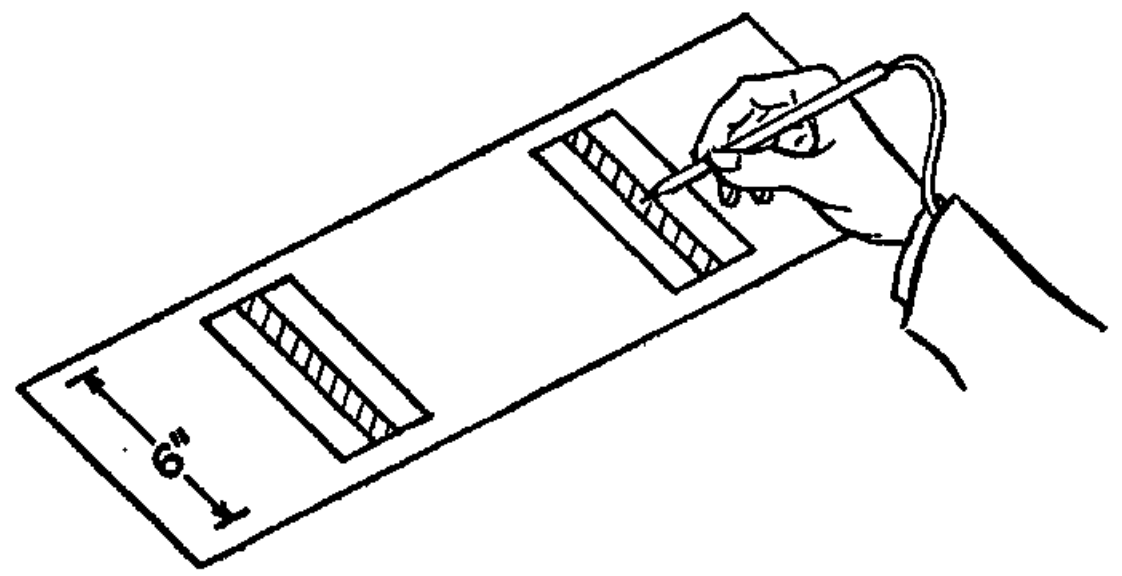
\includegraphics[width=\textwidth]{figures/ch2/fitts}
			\caption{La première expérience ayant mené Paul Fitts à la  définition empirique de la loi du même nom. Deux triplets de plaques étaient séparés d'une certaine distance. Les sujets devaient, avec leur stylet \og tapoter \fg{} alternativement les deux plaques centrales de chaque triplet, hachurées sur ce schéma, sans toucher les plaques adjacentes. On pouvait faire varier la largeur des plaques ciblées, ainsi que la distance entre elles. Crédit : Paul M. Fitts~\cite{fitts1954information}.}
			\label{fig:fitts}
		\end{subfigure}
		~
		\begin{subfigure}[t]{0.40\textwidth}
			\centering
			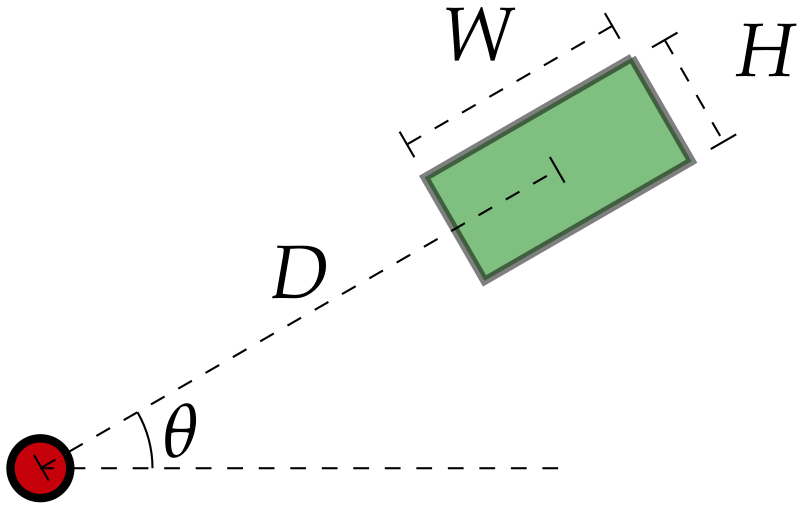
\includegraphics[width=\textwidth]{figures/ch2/theta}
			\caption{Angle $\theta$ pris en compte par~\cite{murata2001extending} dans une version étendue de la loi de Fitts, présentée dans l'équation~\ref{eq:murata}. Le disque rouge représente le curseur, tandis que le rectangle vert représente la cible, située à une distance $D$ du curseur, avec sa largeur $W$ et sa hauteur $H$. Crédit : \cite{casallas2015prediction}.}
			\label{fig:theta}
		\end{subfigure}
		\caption{}
		\label{fig:fittstheta}
	\end{figure}
	
	Paul M. Fitts a donc pu déduire de cette étude la loi qui porte son nom, et que l'on peut décrire par les équations~\ref{eq:fitts} et~\ref{eq:fittsID}.
	
	\begin{equation}
		\label{eq:fitts}
		MT = a + bID
	\end{equation}
	
	\begin{equation}
		\label{eq:fittsID}
		ID = \log_2\left(\frac{2D}{W} \right)
	\end{equation}
	
	Dans l'équation~\ref{eq:fitts}, $MT$ représente le temps de mouvement, $a$ et $b$ sont des constantes déterminées empiriquement. Dans l'équation~\ref{eq:fittsID}, $ID$ représente l'indice de difficulté, $D$ représente l'amplitude du mouvement, c'est-à-dire la distance entre la cible et le point de départ du mouvement, tandis que $W$ représente la largeur de la cible. La partie la plus intéressante de cette équation est l'indice de difficulté. C'est la seule partie variable, et c'est celle qui, comme son nom l'indique, détermine la difficulté de la tâche. Cet indice est aisé à comprendre intuitivement : plus l'amplitude du mouvement nécessaire est grande, plus la tâche sera difficile ; plus la largeur de la cible est grande, plus la tâche sera facile.
	
	Pour l'indice de difficulté, MacKenzie propose une formulation de l'indice de difficulté dite de Shannon, inspirée de la théorie de l'information proposée par ce dernier~\cite{mackenzie1989note}. Cette formulation est fournie dans l'équation~\ref{eq:shannon}.
	
	\begin{equation}
		\label{eq:shannon}
		ID = \log_2\left(\frac{D}{W} + 1\right)
	\end{equation}
	
	\subsection{Extensions de la loi de Fitts}
	L'étude de Paul M. Fitts portait sur un dispositif mécanique simple, mais sa loi s'applique aussi bien aux périphériques de saisie classiques (souris, \emph{joysticks}, etc.)~\cite{card1978evaluation}. Mieux, alors qu'elle fut d'abord énoncée pour des mouvements sur une seule dimension, elle loi s'étend aisément au plan~\cite{card1978evaluation, mackenzie1992extending}, éventuellement en tenant compte de la forme de la cible~\cite{accot2003refining}, ou même à l'espace tridimensionnel~\cite{murata2001extending}. On peut également généraliser la loi de Fitts pour modéliser des tâches de tracé de trajectoires~\cite{accot1997beyond, accot1999performance}.
	
	Bien que la loi de Fitts soit d'une élégante simplicité et d'une utilité évidente pour modéliser les performances de sélection, de nombreuses formulations plus ou moins différentes existent, et leurs mérites respectifs font débat~\cite{casallas2015prediction}. Certaines formulations peuvent, par exemple, tenir compte de l'angle $\theta$ entre le vecteur qui va du curseur à la cible et un vecteur horizontal orienté vers la droite (cf. la figure~\ref{fig:theta}). C'est le cas de la formulation de~\cite{murata2001extending} exposée dans l'équation~\ref{eq:murata}.
	
	\begin{equation}
		\label{eq:murata}
		ID = \log_2\left(\frac{D}{W} + 1\right) + c \sin \theta
	\end{equation}
	
	D'autres versions tiennent compte simultanément de la forme de la cible et de cet angle $\theta$~\cite{appert2008evaluation, grossman2004pointing}.
	
	\subsection{Loi de Fitts et cibles mobiles}
	La recherche sur la loi de Fitts appliquée aux cibles mobiles, comparativement aux travaux sur les cibles statiques, est très pauvre~\cite{casallas2015prediction}. Elle n'est pas inexistante~\cite{jagacinski1980test, hoffmann1991capture, hajri2011moving} mais très limitée, et elle s'intéresse rarement à la nature du mouvement des cibles, surtout quand ce mouvement est imprévisible.
	
	De fait, les modèles développés dans les travaux de Jagacinski \emph{et al.}~\cite{jagacinski1980test} ou d'Al Harji \emph{et al.}~\cite{hajri2011moving}, par exemple, font l'hypothèse de cibles de vitesse et de direction constantes. La loi de Fitts étendue par Jagacinski \emph{et al.} est présentée dans l'équation~\ref{eq:jagacinski}, où $CT$ est le temps de sélection, $D$ et $W$ sont toujours la distance à la cible et sa largeur, $V$ est la vitesse de la cible, tandis que $c$, $d$ et $e$ sont des constantes réelles.
	
	\begin{equation}
		\label{eq:jagacinski}
		CT = c + dD + e(V + 1) \left(\frac{1}{W} - 1\right)
	\end{equation}
	
	Les travaux d'Al Harji \emph{et al.}~\cite{hajri2011moving} vont plus loin en tenant compte de la direction de la cible. Les auteurs ont développé deux modèles basés sur ce principe. Le premier est défini par l'équation~\ref{eq:hajriC2}, où $\vec{F}$ est un vecteur déterminé empiriquement, $\vec{D}$ est le vecteur distance entre le curseur et la cible, $\vec{V}$ est le vecteur de vélocité de la cible, et $\vec{R} = \frac{1}{2} \begin{pmatrix}
	W \\ H \\
	\end{pmatrix}$.
	
	Le second est défini par l'équation~\ref{eq:hajriVW}, où $f_{W'}(\theta)$ est un paramètre empirique dépendant de $\theta$, l'angle formé par la direction du mouvement de la cible et l'horizontale. De même $K$ est un paramètre empirique. $D$ est la distance entre le curseur et la cible, $V$ est la vitesse de la cible, et $W'$ est sa largeur dans la direction du mouvement.
	
	\begin{equation}
		\label{eq:hajriC2}
		ID_{C2} = \log_{2}\left(\abs*{\vec{F} \frac{\vec{D}+\vec{V}}{\vec{R}-\vec{V}}} + 1 \right)
	\end{equation}
	
	\begin{equation}
		\label{eq:hajriVW}
		ID_{VWtW'\theta} = \log_{2}\left( f_{W'}(\theta) \left( \frac{D \pm \frac{V}{K}}{\frac{W'}{2} - \frac{V}{K}} \right) \right)
	\end{equation}
	
	Les corrélations entre ces indices de difficulté et les temps de sélection mesurés par Al Hajri \emph{et al.} sont présentées sur la figure~\ref{fig:holdID}, où l'on observera qu'elles sont très fortes. Néanmoins, ces travaux ne portent que sur des cibles dont la vitesse et la direction sont constantes.
	
	\begin{figure}[!htb]
		\centering
		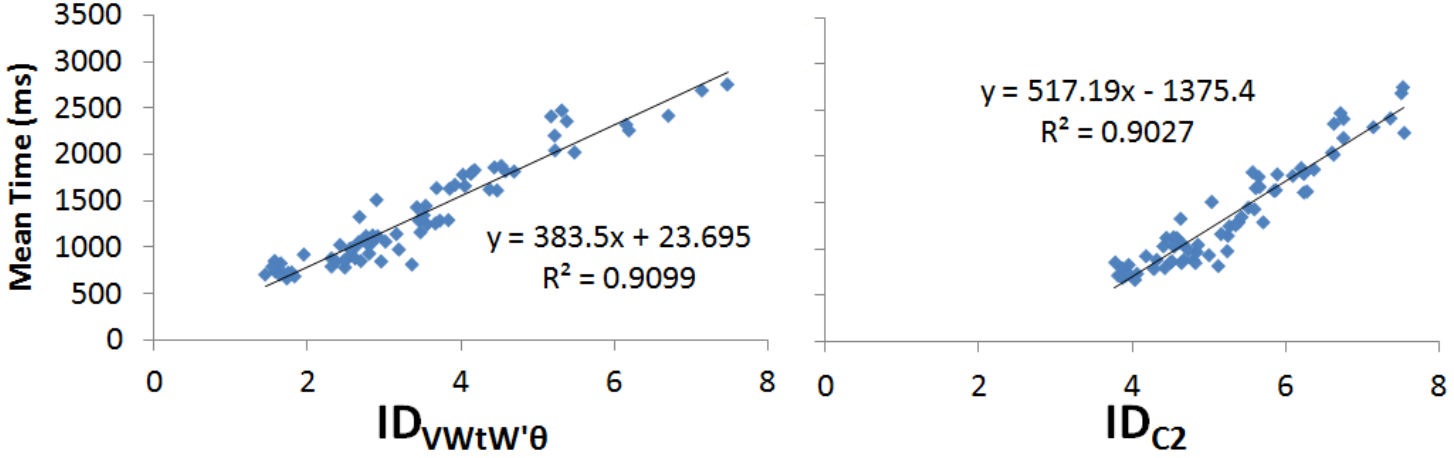
\includegraphics[width=\textwidth]{figures/ch2/holdID}
		\caption[ID vs. nature du mouvement et temps de sélection]{Temps de sélection en fonction des indices de difficulté développés par Al Harji \emph{et al.} Les deux indices sont très fortement corrélés avec les temps de sélection mesurés (sans aucune assistance à la sélection). Crédit : \cite{hajri2011moving}.}
		\label{fig:holdID}
	\end{figure}
	
	Casallas~\cite{casallas2015prediction} a également développé un modèle de prédiction du temps de sélection pour les cibles mobiles, détaillé dans l'équation~\ref{eq:casallas}, où $MT$ est le temps de mouvement, $a_{V}$, $b_{V}$, $c_{V}$ et $d_{V}$ sont des coefficients dépendant linéairement de la vitesse $V$, $D_{m}$ et $D_{s}$ sont les longueurs des composantes orthogonales de $\vec{D}$, le vecteur du curseur à la cible (voir la figure~\ref{fig:casallas}).
	
	\begin{equation}
		\label{eq:casallas}
		MT = a_{V} + b_{V}\sqrt{D_{s}} +  c_{V}\sqrt{D_{m}} + d_{V} \log_{2} \left( \frac{2D_{m}}{W} \right)
	\end{equation}
	
	Dans une évaluation en 3D, l'auteur observe d'une part que l'effet de la vitesse est plus fort que celui de toutes les autres variables, et d'autre part qu'elle réduit l'écart-type des temps de sélection mesurés à mesure qu'elle croît. Il mesure même un très bon ajustement de son modèle aux résultats mesurés, avec le coefficient de détermination $R^{2} \in [0,89 ; 0,96]$.
	
	Il convient cependant de noter un point très spécifique à cette évaluation : les cibles mobiles se dirigeaient toutes \emph{vers} l'utilisateur --- plus ou moins directement. De fait, l'augmentation de la vitesse \emph{diminue} le temps de sélection, puisqu'elle réduit la distance à parcourir pour l'utilisateur, dans un mouvement rectiligne, donc relativement aisé à prédire et anticiper. Ce résultat au demeurant intéressant ne saurait donc suffire à modéliser les performances de sélection pour les cibles mobiles de mouvements quelconques.
	
	\begin{wrapfigure}{O}{0.5\textwidth} % Capital O makes the figure float, because that's totally intuitive and obvious.
		\centering
		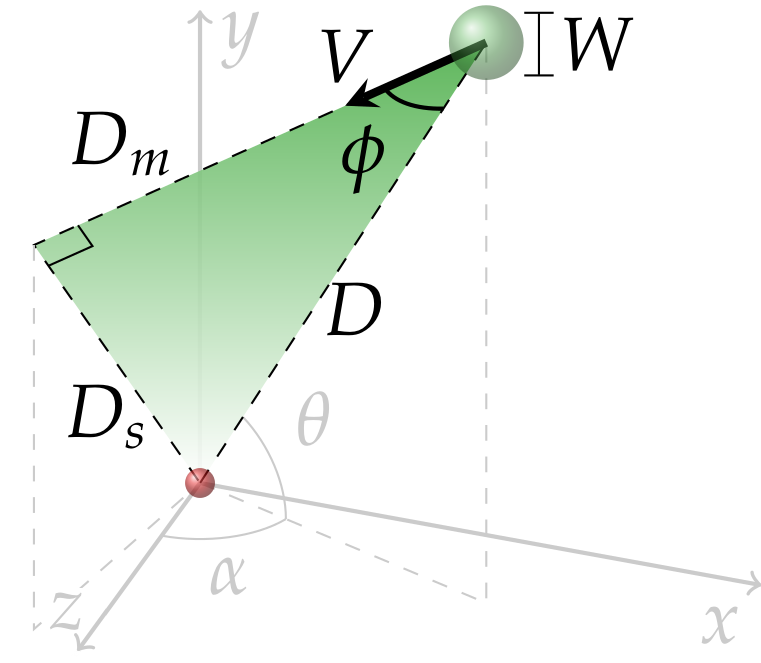
\includegraphics[width=0.46\textwidth]{figures/ch2/casallas}
		\caption[Paramètres du modèle de Casallas]{Modèle de Casallas. $\vec{D}$ est le vecteur du curseur (rouge) à la cible (verte), $\vec{D} = \vec{D_{m}} + \vec{D_{s}}$ où $\vec{D_{m}}$ est la projection de $\vec{V}$ sur $\vec{D}$, et $\vec{D_{s}}$ est la composante de $\vec{D}$ orthogonale à $\vec{D_{m}}$. Crédit : \cite{casallas2015prediction}.}
		\label{fig:casallas}
	\end{wrapfigure}
	
	D'autres travaux s'attachent à développer des techniques de sélection de cibles mobiles \og quelconques \fg{} --- c'est-à-dire de direction et de vitesse potentiellement changeantes --- sans nécessairement s'attarder sur les aspects théoriques~\cite{hasan2011comet, ortega2013hook}, et donc sans chercher à étendre la loi de Fitts.
	
	Celle-ci demeure donc, à notre connaissance, incapable de modéliser la difficulté de sélection de cibles mobiles dont la direction peut changer de façon aléatoire, ce qui la rend d'une utilité discutable pour certaines des applications identifiées plus haut, et particulièrement pour les simulations moléculaires interactives, caractérisées par l'imprévisibilité des mouvements de leurs cibles.
	
	\subsection{Complexité du mouvement : phases balistique et de correction}
	Woodworth~\cite{woodworth1899accuracy} fut à notre connaissance le premier à identifier deux phases dans le mouvement ciblé : une impulsion initiale et une phase de contrôle. Welford~\cite{welford1968fundamentals} fit la même observation et nota par ailleurs que la première phase, visant à couvrir la distance nécessaire, était plus rapide, tandis que la seconde, celle de visée, était plus courte~\cite{mackenzie1987three}. Il remarqua de plus, et de même que Crossman et Goodeve~\cite{crossman1983feedback}, que la première phase était \emph{balistique} et qu'à la seconde s'ajoutait un processus de contrôle visuel.
	
	Cela s'observe concrètement dans le profil de vitesse d'un curseur en fonction du temps au cours d'un mouvement ciblé, par exemple de sélection. La phase balistique est caractérisée par une forte croissance suivie d'une forte décroissance de la vitesse, dans un profil pouvant rappeler une cloche ; puis la phase de correction suit, et se distingue par de faibles mais potentiellement nombreuses et surtout rapides oscillations, comme l'illustre la figure~\ref{fig:ballistic}.
	
	\begin{figure}[!htb]
		\centering
		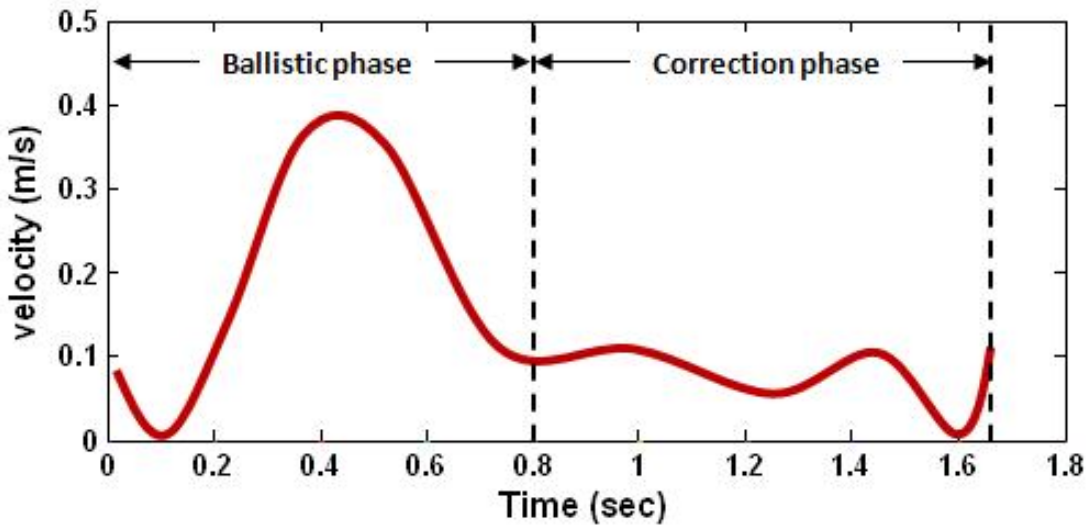
\includegraphics[width=0.75\textwidth]{figures/ch2/ballistic}
		\caption[Profil de vitesse -- phases balistique et de correction]{Vitesse du pointeur en fonction du temps au cours d'un mouvement ciblé. La vitesse croît fortement puis décroît de même au cours de la phase balistique, puis connaît de petites oscillations au cours de la phase de correction. Crédit : \cite{liu2009designing}.}
		\label{fig:ballistic}
	\end{figure}
	
	Langolf \emph{et al.}~\cite{langolf1976investigation} ont de plus montré que \og le mouvement entier vers le centre de la cible devient plus lent quand les tolérances sur la cible [i.e. sa largeur] diminuent \fg{}, ce qui est cohérent avec les travaux de Crossman et Goodeve~\cite{crossman1983feedback}, Marteniuk \emph{et al.}~ \cite{marteniuk1987constraints}, ainsi que ceux de Soechting~\cite{soechting1984effect}. Ce dernier remarqua par ailleurs qu'avec de petites cibles, la phase balistique était plus courte, et de fait la phase de correction en était d'autant rallongée.
	
	La conclusion générale de ces travaux est que la précision requise par un mouvement influe non seulement sur son temps global de complétion, mais également sur l'ensemble de la trajectoire, et notamment sur le profil de vitesse du curseur en fonction du temps. Dès lors, nous pouvons formuler l'hypothèse que les difficultés inhérentes à la sélection de cibles mobiles peuvent être assimilées à un besoin accru de précision, et que par conséquent, un effet comparable pourra être observé sur les trajectoires des curseurs.
	
	Nous reviendrons dans les chapitres suivants sur cette hypothèse.
	
\section{Techniques pour la sélection de cibles statiques}
	Commençons par examiner les techniques conçues pour les cibles statiques, mais précisons au préalable qu'elles sont toutes utilisables avec des cibles mobiles, avec divers degrés d'efficacité.

\subsection{Curseurs zonaux}
	Un curseur zonal substitue au curseur ordinaire, qui est réduit à un point, une zone de sélection~\cite{kabbash1995prince, worden1997making}. Lorsque la cible est petite, les performances de sélection ne sont donc plus limitées par sa taille, mais par la taille du curseur. De plus, la distance effective entre le curseur et la cible est légèrement réduite, puisqu'il faut la mesurer à partir de la limite de la zone de sélection, et non depuis son centre.
	
	\subsubsection{\emph{Prince}}
	La technique \emph{Prince}~\cite{kabbash1995prince} consiste à utiliser un rectangle comme curseur de sélection. Les auteurs ont notamment répliqué la fameuse expérience de Fitts en l'inversant : au lieu d'un point comme curseur et de cibles \og larges \fg{} , ils optèrent pour un curseur large et des cibles ponctuelles, comme l'illustre la figure~\ref{fig:princeCursor}.
	
	\begin{figure}[!htb]
		\begin{subfigure}[t]{0.56\textwidth}
			\centering
			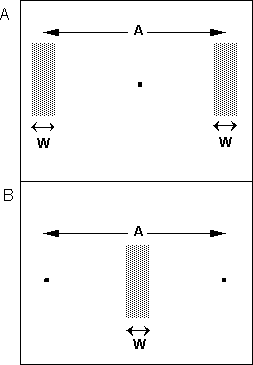
\includegraphics[width=\textwidth]{figures/ch2/princeCursor}
			\caption{À gauche, une représentation schématique de l'expérience de Fitts~\cite{fitts1954information} : un curseur ponctuel est déplacé pour atteindre deux cibles d'aire non nulle. À droite, l'expérience analogue menée dans~\cite{kabbash1995prince}, où le curseur est zonal et les cibles sont ponctuelles.}
			\label{fig:princeCursor}
		\end{subfigure}
		~
		\begin{subfigure}[t]{0.42\textwidth}
			\centering
			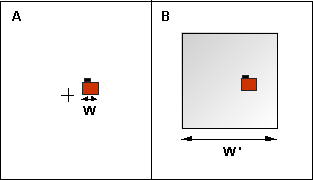
\includegraphics[width=\textwidth]{figures/ch2/princeSelection}
			\caption{Application de la technique \emph{Prince} (à droite) à un cas de sélection pratique, avec pour cible une icône d'aire non nulle ; à gauche, un curseur classique est utilisé.}
			\label{fig:princeSelection}
		\end{subfigure}
		\caption[\emph{Prince}, curseur et sélection]{Crédit : \cite{kabbash1995prince}.}
		\label{fig:princeCursorSelection}
	\end{figure}

	Les auteurs ont pu constater que la loi de Fitts s'appliquait bien à cette configuration, de fait sensiblement identique à celle évaluée par Fitts. Naturellement, dans un environnement de bureau classique, les cibles ne sont pas ponctuelles, mais généralement des icônes ou des boutons d'aire non nulle, comme sur la figure~\ref{fig:princeSelection}, et ce quel que soit le curseur utilisé. De fait, en utilisant un curseur de largeur $W'$, c'est $W'$ qui détermine la difficulté de sélection et non plus la largeur $W$ de la cible (si $W' > w$). Avec un curseur suffisamment gros, l'indice de difficulté peut être considérablement réduit.
	
	La technique \emph{Prince} présente également l'avantage de permettre la sélection de plusieurs cibles d'un coup si elles sont incluses dans le curseur, mais cet avantage reflète une limitation de \emph{Prince}, car il peut dans ces cas-là y avoir ambiguïté si l'utilisateur ne souhaite sélectionner qu'une seule cible.
	
	\subsubsection{\emph{(Sticky) Area Cursor}, \emph{stickiness} et adaptativité}
	Une solution à ce problème d'ambiguïté est proposée par Worden \emph{et al.}~\cite{worden1997making} : lorsqu'un curseur zonal recouvre plusieurs cibles, le curseur devient en pratique un curseur ponctuel, et seul son centre est actif, comme l'illustre la figure~\ref{fig:areaCursor}.
	
	\begin{figure}[!htb]
		\centering
		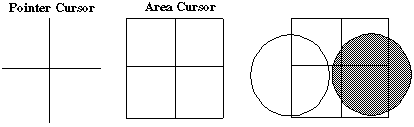
\includegraphics[width=0.70\textwidth]{figures/ch2/areaCursor}
		\caption[\emph{Area Cursor} avec \emph{hot spot}]{Un curseur zonal dont seul le centre, marqué par l'intersection de deux segments, demeure actif lorsque le curseur chevauche plusieurs cibles. Crédit : \cite{worden1997making}.}
		\label{fig:areaCursor}
	\end{figure}
	
	Cette technique simple permet de tirer parti des avantages d'un curseur zonal quand la densité de cibles est suffisamment faibles, sans pour autant souffrir de ses inconvénients lorsqu'elle est élevée, puisque l'on revient alors à un simple curseur ponctuel.
	
	\paragraph{\emph{Stickiness}.}
	À cette solution, Worden \emph{et al.} ont ajouté l'usage de \emph{stickiness} adaptative pour les icônes. Un curseur est dit \emph{sticky} si, lorsqu'il s'approche d'une icône, celle-ci devient \og collante \fg{}. En pratique, le ratio de sensibilité du curseur (la quantité du curseur par rapport à la quantité de mouvement du périphérique de saisie) diminue, ce qui permet d'une part de ralentir le curseur automatiquement, et d'autre part d'affiner les mouvements correctifs permettant la sélection d'une cible lors de son approche.
	
	Le problème des cibles collantes est que lorsque leur densité est élevée, donc en présence de nombreux distracteurs, la trajectoire du curseur se trouve fortement perturbée par ceux-ci, ce qui peut être contre-productif, ou du moins limiter les bénéfices de cette technique. La solution proposée par Worden \emph{et al.} est de ne rendre les cibles collantes que lorsque le curseur est à moins de 30~\%{} de la vitesse maximale qu'il a atteinte au cours de la tâche de sélection courante. L'hypothèse est qu'une sélection commence par une phase de mouvement très rapide et ample, suivie de petits mouvements correctifs plus lents, et que le curseur sera donc relativement lent près de la cible réellement visée par l'utilisateur.
	
	L'\emph{Area cursor}, en particulier complémenté par des cibles collantes et un gain adaptatif, permet un gain de performances important, en particulier avec des utilisateurs âgés, comme le détaille le tableau~\ref{tab:areaCursor}.
	
	\begin{table}
	\centering
	\begin{tabular}{l c c c c}
										& \multicolumn{2}{c}{Jeunes}	&	\multicolumn{2}{c}{Âgés}			\\
										& Temps (ms)	& Taux de succès	& Temps (ms)	& Taux de succès	\\
		Pointeur seul					& 759			& 95,0				& 1893			& 95,0				\\
		Pointeur collant				& 712			& 97,4				& 1869			& 96,3				\\
		Pointeur adaptatif				& 743			& 97,7				& 1485			& 95,5				\\
		\emph{Area cursor} seul			& 639			& 96,9				& 1658			& 96,3				\\
		\emph{Area cursor} collant		& 596			& 97,9				& 1596			& 97,7				\\
		\emph{Area cursor} adaptatif	& 591			& 99,0				& 1203			& 97,9				\\
	\end{tabular}
	\caption[\emph{Area cursor} -- performances]{Performances mesurées pour un \emph{Area cursor} avec des cibles collantes, ainsi qu'avec des cibles collantes et un gain adaptatif en fonction de la vitesse du curseur. Les résultats sont comparés avec un curseur ponctuel dans les mêmes conditions, avec des sujets jeunes (23,4 ans en moyenne) et plus âgés (70,1 ans en moyenne). Les performances sont rapportées par le temps de sélection ainsi que le taux de succès (pourcentage de sélections réussies). Le curseur zonal avec cibles collantes et gain adaptatif permet les meilleures performances, tant avec des sujets jeunes que plus âgés, mais c'est au sein du second groupe que l'apport est le plus important. Données tirées de~\cite{worden1997making}.}
	\label{tab:areaCursor}
	\end{table}

	\subsubsection{\emph{Bubble Cursor}}
	La technique \emph{Bubble Cursor} consiste à agrandir dynamiquement un curseur zonal (représenté par un disque) jusqu'à ce qu'il atteigne la cible la plus proche. Mathématiquement, cela revient à construire un diagramme de Voronoï des cibles et à s'appuyer dessus pour la sélection : le \emph{Bubble Cursor} est toujours dans une et une seule cellule du diagramme, et peut sélectionner la cible correspondante, comme l'illustrent les figures~\ref{fig:bubble} et~\ref{fig:voronoi}. De fait, dans sa version pure, il n'est capable de sélectionner que des cibles, pas l'espace entre celles-ci.	

	\begin{figure}[!htb]
		\begin{subfigure}[t]{0.49\textwidth}
			\centering
			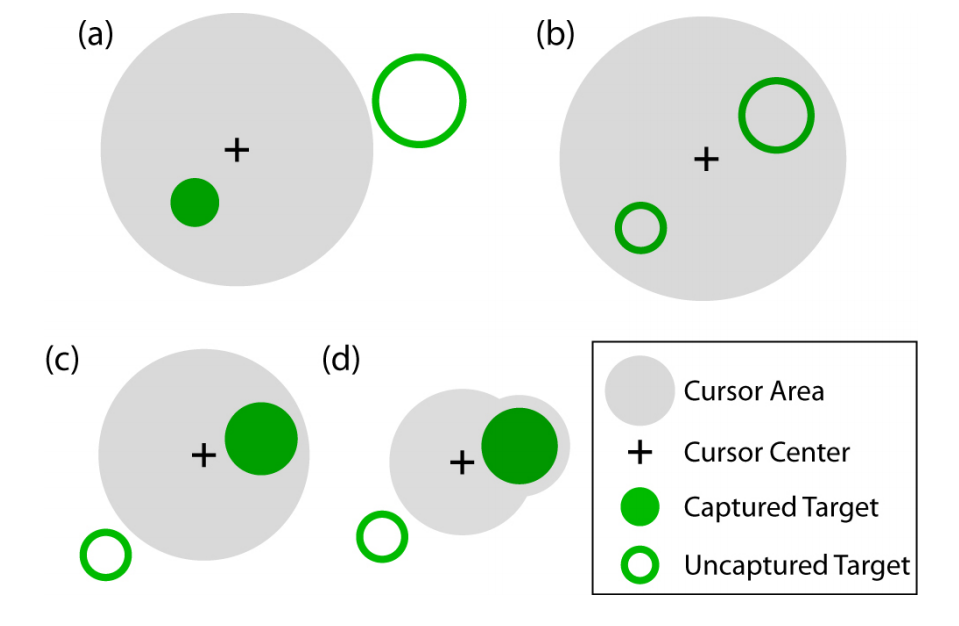
\includegraphics[width=\textwidth]{figures/ch2/bubble}
			\caption{\emph{Bubble Cursor} en (a, c, d) par opposition à un curseur zonal (b). Dans le cas (b), le curseur zonal ne permet pas aisément de choisir entre les deux cibles qui se trouvent dans la zone de sélection. Mais le \emph{Bubble Cursor} s'adapte (c et d). Dans le cas (d), la cible n'est pas entièrement recouverte par le disque du curseur, mais elle l'est partiellement, et pour représenter visuellement que c'est suffisant à sa sélection, le curseur est localement étendu pour l'englober.}
			\label{fig:bubble}
		\end{subfigure}
		~
		\begin{subfigure}[t]{0.49\textwidth}
			\centering
			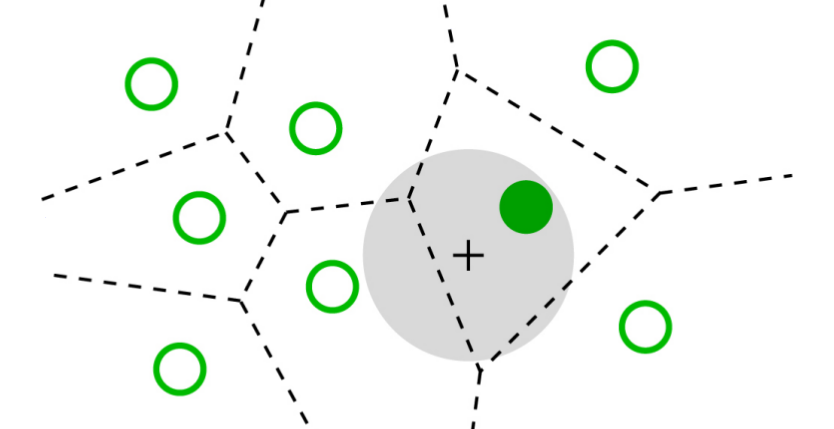
\includegraphics[width=\textwidth]{figures/ch2/voronoi}
			\caption{Diagramme de Voronoï définissant les cellules associées à chaque cible. C'est un découpage du plan (pavage) en cellules à partir d'un ensemble discret de points (\emph{germes}). Chaque cellule enferme un seul germe, et forme l'ensemble des points plus proches de ce germe que des autres. Ici, les frontières d'activation de chaque cible, donc sa largeur effective, sont définies par sa cellule.}
			\label{fig:voronoi}
		\end{subfigure}
		\caption[\emph{Bubble Cursor}]{\emph{Bubble Cursor}. Crédit : \cite{grossman2005bubble}.}
		\label{fig:bubbleVoronoi}
	\end{figure}
	
	\begin{wrapfigure}{O}{0.5\textwidth} % Capital O makes the figure float, because that's totally intuitive and obvious.
		\centering
		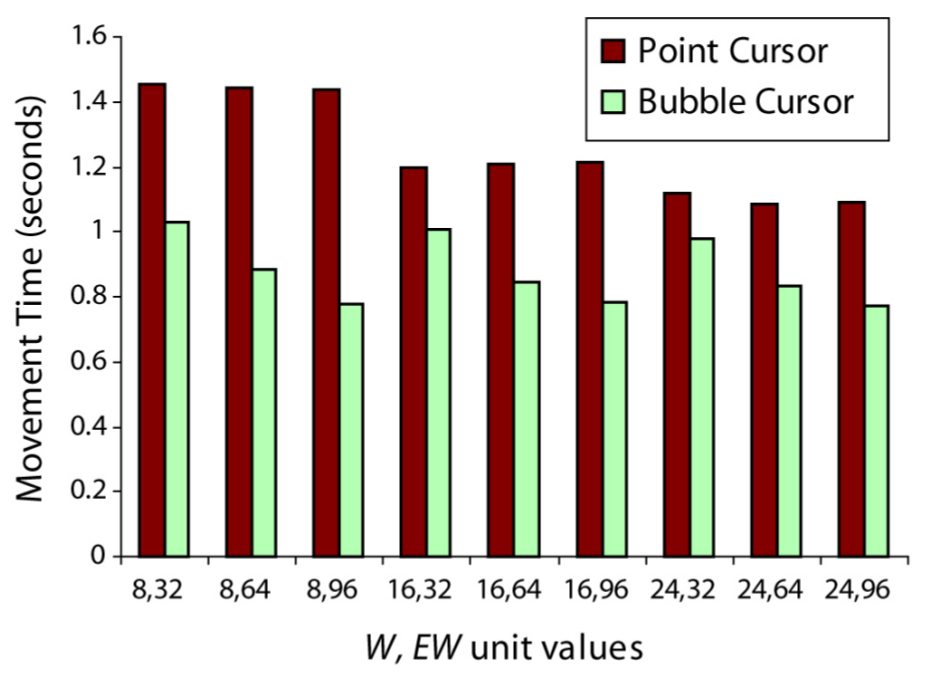
\includegraphics[width=0.46\textwidth]{figures/ch2/bubbleResults}
		\caption[\emph{Bubble Cursor} --  performances]{Temps de pointage avec et sans le \emph{Bubble Cursor}, en fonction de $W$ et $EW$, où $W$ est la largeur réelle de la cible, et $EW$ sa largeur effective. Le \emph{Bubble Cursor} améliore les performances, dépend de $EW$ bien plus que de $W$. Crédit : \cite{grossman2005bubble}.}
		\label{fig:bubbleResults}
	\end{wrapfigure}
	
	Grossman et Balakrishnan ont montré que les performances de sélection avec le \emph{Bubble Cursor} suivent la loi de Fitts, à condition de remplacer la largeur de la cible par sa largeur effective, c'est-à-dire la largeur de sa cellule dans le diagramme de Voronoï~\cite{grossman2005bubble}, cf. la figure~\ref{fig:bubbleResults}. Le \emph{Bubble Cursor} peut être mis en œuvre en 2D aussi bien qu'en 3D~\cite{vanacken2007exploring}.

	\paragraph{Instabilité.}
	Un inconvénient de cette technique est le fait que le curseur peut rapidement croître et décroître à mesure qu'il s'approche et s'éloigne de plusieurs cibles successives. Cela peut représenter une source de distraction visuelle, en particulier quand les cibles elles-mêmes sont mobiles, \emph{a fortiori} si elles sont rapides. De plus, attendu que le \emph{Bubble Cursor} agrandit la largeur effective des cibles à la mesure de leur cellule de Voronoï, il est moins efficace en environnement dense, où les cellules de Voronoï sont plus petites. Le \emph{Bubble Cursor} montre donc ses limites face à des cibles potentielles nombreuses, mobiles et rapides.
	
	Un autre inconvénient (potentiellement majeur) du \emph{Bubble Cursor} est intrinsèquement lié à son mode de fonctionnement : il partage l'espace de sélection en un diagramme de Voronoï, où toute partie de l'espace fait partie de la zone de sélection d'une cible. Par conséquent, il n'existe plus d'espace \og vide \fg{} dans lequel on pourrait utiliser le périphérique de saisie pour effectuer une opération indépendante des cibles, par exemple ouvrir un menu contextuel.
	
	\subsubsection{\emph{Silk Cursor}}
	Le \emph{Silk Cursor}~\cite{zhai1994silk} est analogue aux curseurs zonaux décrits plus haut, mais étendu à la 3D. Il s'agit donc d'un volume semi-transparent que l'utilisateur peut utiliser pour sélectionner un objet en déplaçant le volume de telle sorte que l'objet soit dedans.
	
	Tel qu'il fut évalué dans~\cite{zhai1994silk}, le \emph{Silk Cursor} doit entièrement englober un objet pour pouvoir le sélectionner ; ainsi, dans l'illustration de la figure~\ref{fig:silk}, le poisson ne peut pas encore être sélectionné. Celui-ci était animé par une combinaison de fonctions sinusoïdales agissant indépendamment sur chacune de ses coordonnées (x,y,z). Ces fonctions sont détaillées par les équations~\ref{eq:silkMotion0}, \ref{eq:silkMotion1} et~\ref{eq:silkMotion2} où $t$ est le temps, $A = 4,55$~cm, $p = 2$, $f_{0} = 0,02$~Hz, 	$\phi_{x}(i)$, $\phi_{y}(i)$ et $\phi_{z}(i)$ sont des nombres pseudo-aléatoires, échantillonés uniformément entre $0$ et $2\pi$. Ces fonctions ont pour but de produire un mouvement lisse (\emph{smooth}) et subjectivement imprévisible~\cite{zhai1993human}.
	
	\begin{align}
		\label{eq:silkMotion0}
		x(t) &= \sum_{i=0}^{5} Ap^{-i} \sin \left( 2\pi{}f_{0}p^{i}t + \phi_{x}(i) \right) \\
		\label{eq:silkMotion1}
		y(t) &= \sum_{i=0}^{5} Ap^{-i} \sin \left( 2\pi{}f_{0}p^{i}t + \phi_{y}(i) \right) \\
		\label{eq:silkMotion2}
		z(t) &= \sum_{i=0}^{5} Ap^{-i} \sin \left( 2\pi{}f_{0}p^{i}t + \phi_{z}(i) \right) - 7.8
	\end{align}
	
	\paragraph{Temps de sélection.}
	Les performances du \emph{Silk Cursor} furent évaluées par Zhai \emph{et al.} en le comparant à un curseur volumique de fonctionnement identique, mais rendu en fil de fer, dans des conditions monoscopiques et stéréoscopiques (voir la figure~\ref{fig:silkPerf}). Comme le supposaient les auteurs, la semi-transparence du curseur permet une forte amélioration du temps de sélection, particulièrement avec un écran monoscopique. De plus, la stéréoscopie réduit le temps de sélection de façon significative, et ce même avec le \emph{Silk Cursor}.
	
	\begin{figure}[!htb]
		\begin{subfigure}[t]{0.38\textwidth}
			\centering
			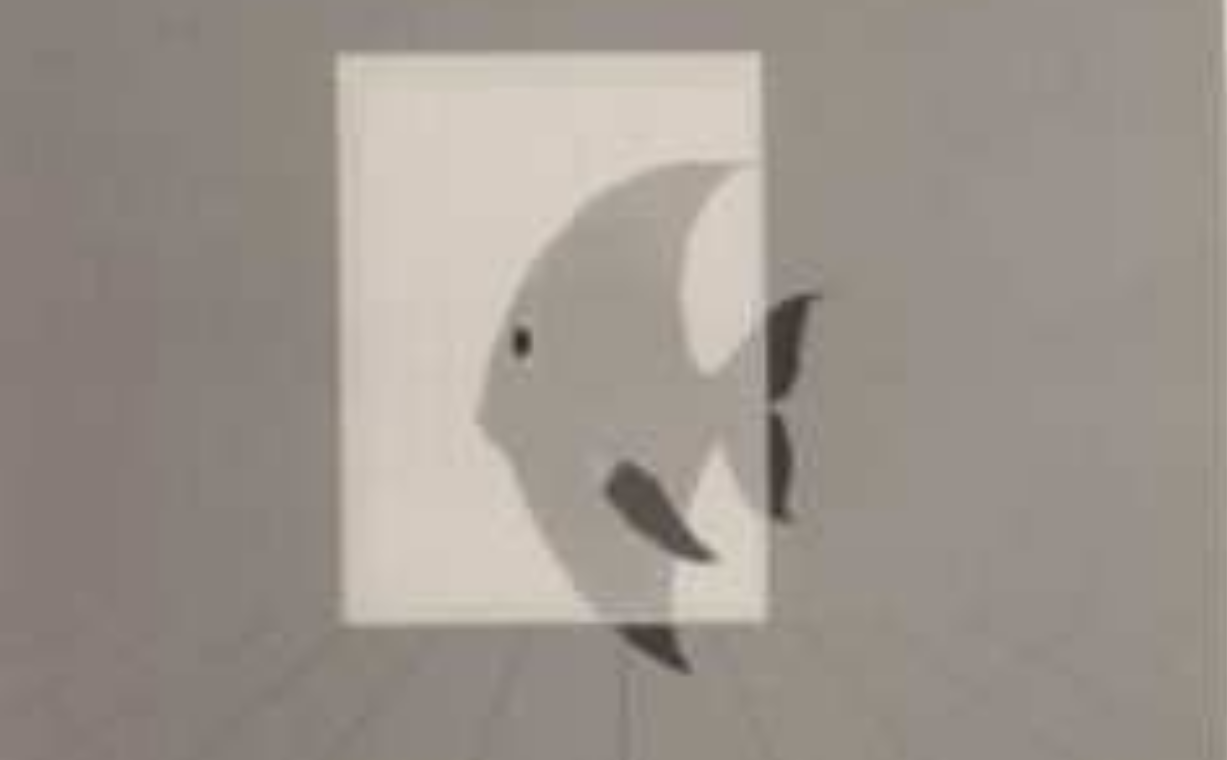
\includegraphics[width=\textwidth]{figures/ch2/silk}
			\caption{Le \emph{Silk Cursor} : l'utilisateur est ici en train d'essayer de sélectionner un poisson, en l'englobant avec le volume du curseur. Quelques parties du poisson ne sont pas incluses dans le volume de sélection, et de fait il ne peut pas encore être sélectionné.}
			\label{fig:silk}
		\end{subfigure}
		~
		\begin{subfigure}[t]{0.60\textwidth}
			\centering
			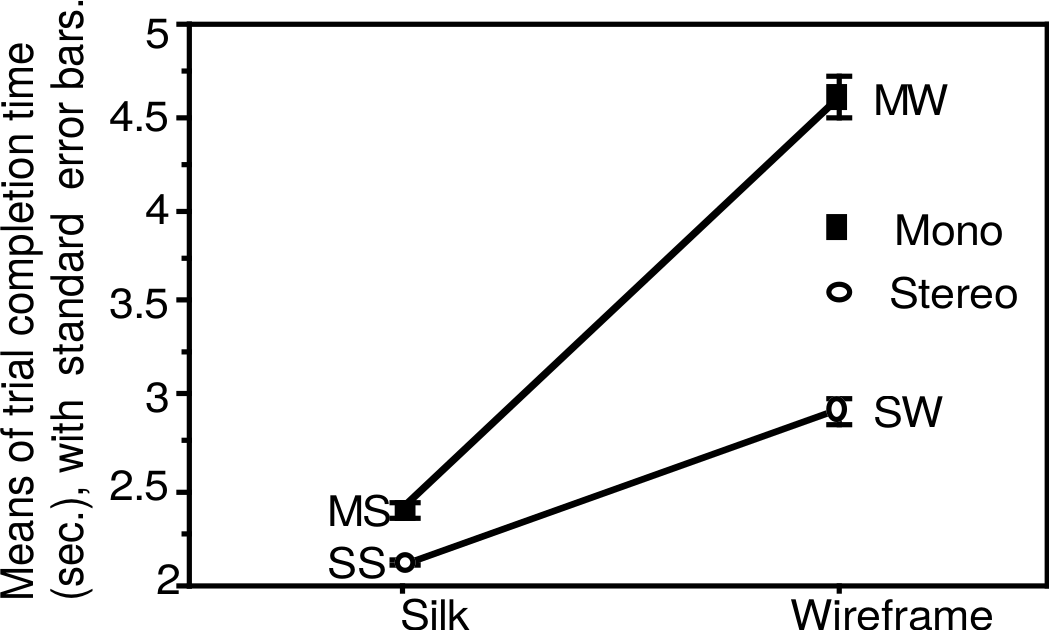
\includegraphics[width=\textwidth]{figures/ch2/silkPerf}
			\caption{Temps de sélection du \emph{Silk Cursor} et d'un curseur volumique en fil de fer. Pour la première lettre, \emph{M} indique une condition monoscopique et \emph{S} indique une condition stéréoscopique ; pour la seconde, \emph{S} désigne le \emph{Silk Cursor}, et \emph{W} correspond au curseur en fil de fer (\emph{wireframe}). La stéréoscopie et le \emph{Silk Cursor} permettent tous deux de fortement réduire le temps de sélection. L'axe des ordonnées ne commence pas à 0.}
			\label{fig:silkPerf}
		\end{subfigure}
		\caption[\emph{Silk Cursor}]{\emph{Silk Cursor}. Crédit : \cite{zhai1994silk}}
		\label{fig:silkCursorPerf}
	\end{figure}
	
	On observera toutefois que la conception de l'évaluation pourrait favoriser ce dernier de façon artificielle, en ce qu'il est nécessaire que l'objet visé soit intégralement inclus dans le curseur volumique, ce qui ne paraît pas indispensable dans l'absolu. Or, en fil de fer, vérifier cela visuellement paraît très difficile, tandis que s'assurer qu'une partie de l'objet est dans le curseur semble plus aisé ; on peut supposer que la différence de difficulté entre ces deux tâches est moindre avec le \emph{Silk Cursor} grâce aux indications fournies par la semi-transparence.
	
	\paragraph{Taux et amplitude des erreurs.}
	Les auteurs ont également évalué les performances du \emph{Silk Cursor} sous l'angle des erreurs, tant leur taux d'occurrence (voir la figure~\ref{fig:silkErrors}) que leur amplitude (voir la figure~\ref{fig:silkErrorMag}). Cette technique de sélection permet donc d'améliorer les temps de sélection, de réduire les occurrences d'erreurs et de diminuer leur amplitude lorsqu'elles se produisent malgré tout.
	
	\begin{figure}[!htb]
		\begin{subfigure}[t]{0.49\textwidth}
			\centering
			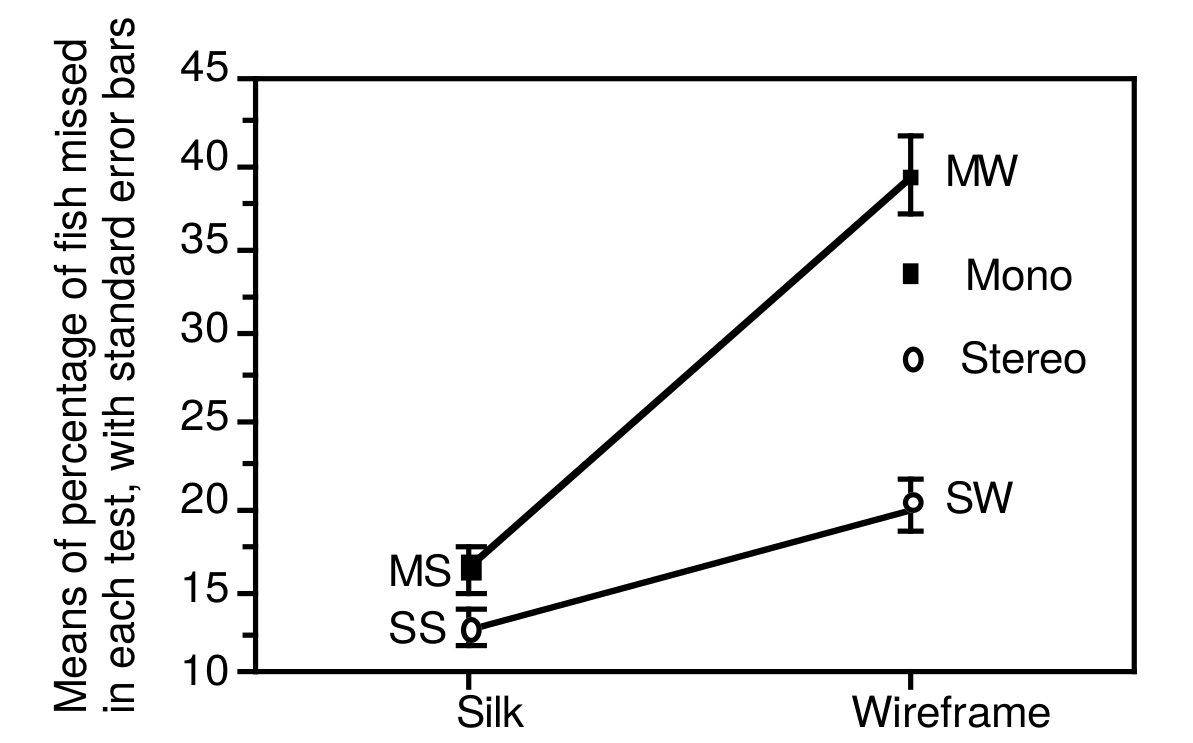
\includegraphics[width=\textwidth]{figures/ch2/silkErrors}
			\caption{Taux d'erreurs du \emph{Silk Cursor} comparé à un curseur volumique rendu en fil de fer. Comme pour les temps de sélection, la stéréoscopie et le \emph{Silk Cursor} améliorent significativement les performances. Les conditions sont indiquées comme sur la figure~\ref{fig:silkPerf}. L'axe des ordonnées ne commence pas à 0.}
			\label{fig:silkErrors}
		\end{subfigure}
		~
		\begin{subfigure}[t]{0.49\textwidth}
			\centering
			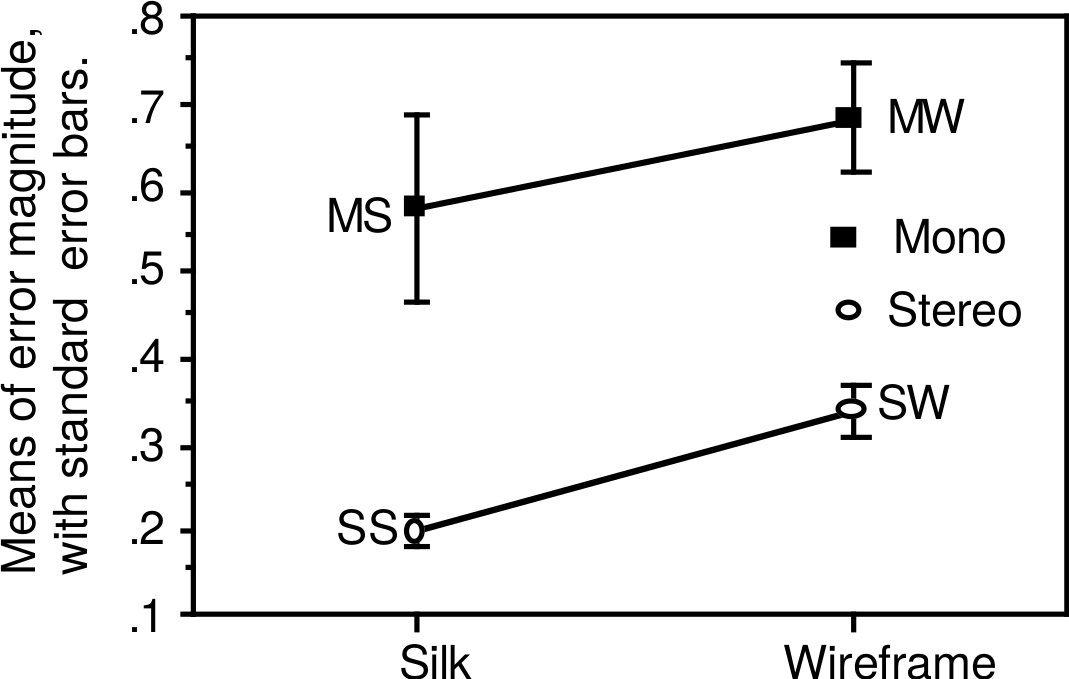
\includegraphics[width=\textwidth]{figures/ch2/silkErrorMag}
			\caption{Amplitude des erreurs du \emph{Silk Cursor} comparé à un curseur volumique en fil de fer. Il s'agit de la distance euclidienne entre la position du curseur et celle souhaitée pour saisir la cible. La stéréoscopie et le \emph{Silk Cursor} améliorent significativement les performances. Les conditions sont indiquées comme sur la figure~\ref{fig:silkPerf}. L'axe des ordonnées ne commence pas à 0.}
			\label{fig:silkErrorMag}
		\end{subfigure}
		\caption[\emph{Silk Cursor} -- erreurs]{\emph{Silk Cursor} -- erreurs. Crédit : \cite{zhai1994silk}}
		\label{fig:SilkErrorsErrMag}
	\end{figure}
	
	Enfin, cette étude menée par Zhai \emph{et al.}~\cite{zhai1994silk} confirme l'intérêt du rendu stéréoscopique pour de telles tâches, et vérifie qu'il apporte toujours un bénéfice tangible lorsqu'il est combiné au \emph{Silk Cursor}.
	
	\paragraph{Impressions subjectives.}
	Zhai \emph{et al.} ont également recueuilli les impressions subjectives des sujets de leur étude, compilées dans la table~\ref{tab:silkImpr}. Le \emph{Silk Cursor} fut évalué très positivement par les utilisateurs, qui ont même préféré sa version monoscopique à la version stéréoscopique du curseur en fil de fer. En stéréoscopie, toutes les impressions subjectives étaient au moins hautes, et souvent très hautes.

	\begin{table}
	\centering
	\begin{tabular}{c | c c c c c}
							& \multicolumn{5}{c}{Impressions subjectives} \\
		Condition			& Très basse	& Basse	& Moyenne	& Haute	& Très haute \bigstrut[b] \\ \hline
		\emph{MonoWire}		& 8				& 2		& 1			&		& \bigstrut[t]	\\
		\emph{MonoSilk}		& 				& 		& 4			& 4		& 4 			\\
		\emph{StereoWire}	& 				& 2		& 7			& 3		& 	 			\\
		\emph{StereoSilk}	& 				& 		& 			& 3		& 9 			\\
	\end{tabular}
	\caption[\emph{Silk Cursor} -- impressions subjectives]{Impressions subjectives du \emph{Silk Cursor}. \emph{MonoWire} et \emph{MonoSilk} sont les conditions monoscopiques en fil de fer et avec le \emph{Silk Cursor} respectivement ; \emph{StereoWire} et \emph{StereoSilk} sont les équivalents respectifs en stéréoscopie. Chaque case contient le nombre de sujets ayant évalué la condition correspondante de la sorte. Le \emph{Silk Cursor} s'illustre par les 9 très hautes appréciations reçues en stéréoscopie. Source :~\cite{zhai1994silk}.}
	\label{tab:silkImpr}
	\end{table}

	\subsubsection{\emph{DynaSpot}}
	Cette lacune du \emph{Bubble Cursor} est une des raisons d'être de la technique \emph{DynaSpot}~\cite{chapuis2009dynaspot}. Celle-ci relie l'aire du curseur à sa vitesse. Le curseur conserve sa taille normale lorsqu'il est lent, mais croît et affecte une plus grande surface quand il se déplace plus vite. De fait il suffit de ralentir pour ramener le curseur à un comportement \og normal \fg{} et pouvoir sélectionner de l'espace vide, par exemple pour ouvrir un menu contextuel, ou agir directement sur l'espace vide, comme l'illustre la figure~\ref{fig:dynaSpot}.
	
	\begin{figure}[!htb]
		\begin{subfigure}[t]{0.49\textwidth}
			\centering
			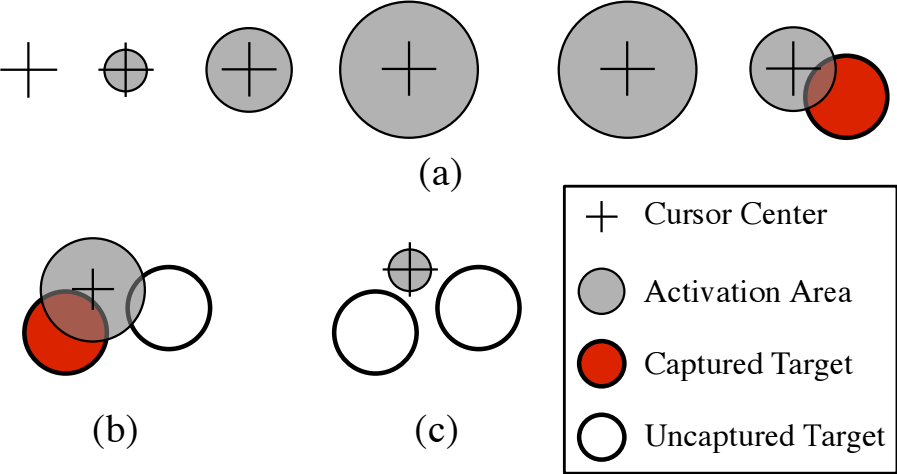
\includegraphics[width=\textwidth]{figures/ch2/dynaSpot}
			\caption{(a) La zone d'activation de \emph{DynaSpot} est couplée à la vitesse du curseur : plus celui-ci est rapide, plus celle-là est grande. (b) Plusieurs objets coupent la zone de sélection : la cible la plus proche du curseur est en sur-brillance et sélectionnée. (c) Quand la zone de sélection ne touche aucun objet, on peut sélectionner l'espace vide.}
			\label{fig:dynaSpot}
		\end{subfigure}
		~
		\begin{subfigure}[t]{0.49\textwidth}
			\centering
			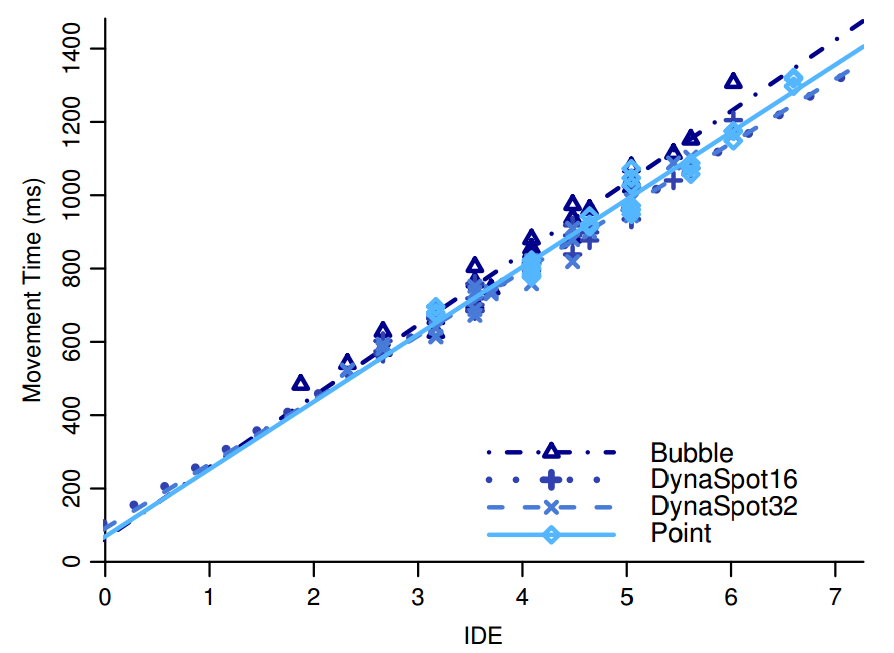
\includegraphics[width=\textwidth]{figures/ch2/dynaResults}
			\caption{Performances (en temps de sélection) du \emph{BubbleCursor}, de \emph{DynaSpot} (2 versions paramétrées différemment) et d'un curseur ordinaire, en fonction de l'ID. Celui-ci est calculé en fonction de la largeur de la cible pour le curseur ordinaire, de la largeur effective pour le \emph{Bubble Cursor} et \emph{DynaSpot}.}
			\label{fig:dynaResults}
		\end{subfigure}
		\caption[\emph{DynaSpot} -- principe et performances]{\emph{DynaSpot} -- principe et performances. Crédit : \cite{chapuis2009dynaspot}.}
		\label{fig:dynaSpotRes}
	\end{figure}
	
	Il n'est donc pas nécessaire de désactiver \emph{DynaSpot} ou de changer de mode explicitement. En ceci, \emph{DynaSpot} comble une des lacunes du \emph{Bubble Cursor}. Chapuis \emph{et al.}~\cite{chapuis2009dynaspot} ont montré que dans la plupart des cas, les performances de \emph{DynaSpot} sont similaires à celles du \emph{Bubble Cursor}. Ces résultats sont résumés dans la figure~\ref{fig:dynaResults}.

	Attendu que la croissance et la décroissance du curseur sont à la fois lentes et prévisibles avec cette technique, le niveau de distraction visuelle est faible. Par ailleurs, il n'est pas nécessaire de connaître la position des cibles potentielles pour appliquer \emph{DynaSpot}, qui ne dépend que de la vitesse du curseur. En cela, cette technique permet de pallier deux autres inconvénients du \emph{Bubble Cursor}.

	\paragraph{Ambiguïté et ralentissements.}
	Le principal inconvénient de cette technique est précisément le fait que le curseur ne tient pas compte des cibles. Par conséquent, à vitesse élevée, sa surface peut en recouvrir plusieurs, et il ne peut déterminer laquelle est la bonne. Il est donc nécessaire de ralentir et d'attendre que le curseur rapetisse suffisamment pour ne toucher qu'une cible. En pratique, cela se produit assez rapidement, et pour les cibles statiques ce n'est pas vraiment gênant. Mais si les cibles sont mobiles, et \emph{a fortiori} rapides, le curseur ne peut s'arrêter, et il peut même être impossible à l'utilisateur de ralentir suffisamment pour que le curseur retrouve une taille permettant la sélection. Ainsi, de même que pour le \emph{Bubble Cursor}, la densité et la vitesse des cibles posent de sérieux problèmes.

	On pourrait toutefois envisager une sélection en deux temps (en cascade) : l'utilisateur pré-sélectionnerait plusieurs cibles lorsque le curseur est gros et rapide, puis devrait choisir parmi les cibles touchées laquelle il veut. Naturellement, le processus de sélection en deviendrait plus lourd et plus long, et pourrait nécessiter de stopper (ou ralentir) les cibles après l'étape de pré-sélection pour que la sélection finale soit réalisable, ou bien encore de zoomer fortement sur l'espace pré-sélectionné. Cette dernière solution est intéressante sur le papier mais pourrait s'avérer peu pratique si les cibles de l'espace pré-sélectionné ont des directions opposées et sont suffisamment rapides pour forcer un \og dézoom \fg{} avant que la sélection finale ne puisse avoir lieu.

	\subsubsection{La densité : un écueil pour les curseurs zonaux}
	Le principal inconvénient d'un curseur zonal se présente lorsque la densité de cibles potentielles est élevée. Si deux cibles sont séparées d'une distance inférieure à la taille de la zone de sélection, il peut être difficile de choisir parmi les deux. Ce problème est illustré par la figure~\ref{fig:bubble}. Il est possible de partiellement pallier ce problème en utilisant une zone plus petite, mais en plus de réduire l'efficacité de la technique, ce n'est certain de fonctionner que si l'on connaît la distance minimale entre deux cibles \emph{a priori}. La figure~\ref{fig:areaCursor} présente une solution possible, qui consiste à n'utiliser que le centre du curseur, mais cela implique la perte de l'avantage fourni par un curseur zonal.
	
	\subsection{Techniques de lancer de rayon (\emph{raycasting})}
	Certaines techniques substituent aux curseurs classiques des rayons ou volumes projetés depuis un point contrôlé par l'utilisateur. Nous allons ici les examiner ensemble.

	\subsubsection{Lancer de rayon (\emph{raycasting}) pur}
	Le \emph{raycasting} est une technique de sélection conceptuellement très simple : un périphérique est utilisé pour lancer un rayon virtuel, généralement le long d'un axe du périphérique. Le rayon peut ensuite croiser un objet, ce qui permet de le sélectionner. Cette technique est parfois appelée \emph{laser gun}~\cite{liang1994jdcad}, et elle est illustrée par la figure~\ref{fig:dCanvas2}.
	
	Elle a plusieurs avantages : elle permet de sélectionner un objet à n'importe quelle distance, sans avoir à se déplacer ; on peut sélectionner un objet très éloigné de la position initiale du curseur sans avoir à faire de grand mouvement, puisqu'il suffit de changer l'orientation du périphérique de pointage, donc d'un simple mouvement de poignet.
	
	Cependant, pour les objets de petite taille apparente, la sélection peut être difficile, car elle requiert une précision angulaire élevée. De plus, si le système de \emph{tracking} qui fournit la position et l'orientation du périphérique de pointage produit un signal bruité, la difficulté de sélection s'en trouve encore accrue. Par conséquent, des techniques dérivées du \emph{raycasting} ont été développées.
	
	Classiquement, on utilisera une technique de cône de sélection, comme par exemple \emph{Spotlight}~\cite{liang1994jdcad}, illustrée par la figure~\ref{fig:spotlight}. Comme le nom l'indique, les techniques de ce typent remplacent le rayon de sélection par un cône dont le sommet est placé sur le périphérique de pointage.
	
	\begin{wrapfigure}{O}{0.5\textwidth} % Capital O makes the figure float, because that's totally intuitive and obvious.
		\centering
		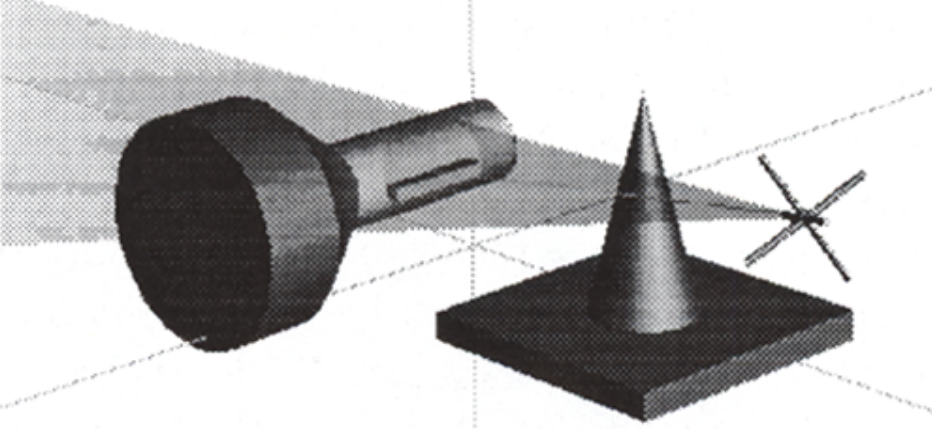
\includegraphics[width=0.46\textwidth]{figures/ch2/spotlight}
		\caption[Cône de sélection : \emph{Spotlight}]{Illustration d'une technique de sélection par cône, baptisée \emph{Spotlight}. Les objets qui se trouvent dans le cône sont des candidats à la sélection : quand il y en a plusieurs, le plus proche de l'axe de révolution du cône est choisi ; en cas de proximité égale, le plus proche du périphérique de pointage est choisi. Crédit : \cite{liang1994jdcad}.}
		\label{fig:spotlight}
	\end{wrapfigure}
	
	Cela facilite la sélection, puisque les gestes n'ont plus besoin d'être aussi précis, mais peut ajouter de l'ambiguïté si deux objets se trouvent dans le cône de sélection. Le cas échéant, cette ambiguïté peut être levée de plusieurs façon, en fonction de la proximité à l'axe de révolution du cône, en fonction de la distance au périphérique de pointage, ou via une intervention directe de l'utilisateur.
	
	Le choix de l'angle du cône est important : plus il sera grand, plus la sélection sera facile mais potentiellement ambiguë ; plus il sera petit, plus la sélection sera difficile mais spécifique. Le choix de cet angle peut éventuellement être paramétrable, permettant à l'utilisateur de choisir ce qui lui convient le mieux, voire de l'ajuster à la volée en cours d'utilisation. Cet ajustement pourrait également être géré automatiquement par le système interactif, par exemple de façon analogue à ce qui est fait avec des pointeurs classiques dans le \emph{Bubble Cursor}~\cite{grossman2005bubble} ou \emph{DynaSpot}~\cite{chapuis2009dynaspot}.
	
	\subsubsection{\emph{Shadow Cone}}
	Le \emph{Shadow Cone}~\cite{steed20043d} est une technique développée spécifiquement pour les \emph{spatially immersive displays} (SID) tels que les CAVE. L'idée est de permettre non seulement une sélection performante dans des conditions \og normales \fg{} mais également de sélectionner des objets lorsque l'utilisateur n'est pas suivi par le SID, et que le rendu n'est pas adapté à sa position, donc incorrect.
	
	Steed et Parker~\cite{steed20043d} identifient ce besoin en partant du constat qu'un SID ne permet généralement de suivre et d'adapter le rendu graphique qu'à une seule personne (mais pas toujours\footnotemark), ce qui implique qu'un deuxième utilisateur ne peut bénéficier d'un rendu adapté, et rencontrera donc des difficultés pour accomplir des tâches collaboratives nécessitant une étape de sélection.
	
	\footnotetext{Le système EVE (Environnement Virtuel Evolutif), permet d'étudier à la fois les aspects multisensoriels et collaboratifs des interactions humaines au sein de mondes virtuels. Les spécificités du système EVE, comme ses dimensions très grandes, une stéréoscopie multi-utilisateurs haute qualité, des rendus haptiques et audio 3D, en font un dispositif unique au monde à la pointe de la technologie dans le domaine de la réalité virtuelle.
	\url{https://www.limsi.fr/index.php/fr/recherche/venise/menuitem-venise-demos-fr}}
	
	Le \emph{Shadow Cone} fonctionne comme un cône de sélection, mais avec une désambiguïsation explicite : lorsque l'utilisateur presse le bouton de son périphérique de pointage, tous les objets dans le cône sont pré-sélectionnés ; puis, l'utilisateur déplace le périphérique et son cône avec, de telle sorte que certains des objets pré-sélectionnés ne sont plus dans le cône. Dès lors qu'ils en sortent, ils ne sont plus pré-sélectionnés, et aucun objet n'est ajouté à la pré-sélection. Quand l'utilisateur relâche le bouton de son périphérique, tous les objets se trouvant encore dans le cône --- et l'ayant toujours été --- sont sélectionnés. Ce fonctionnement est illustré par la figure~\ref{fig:shadow}.
	
	\begin{figure}[!htb]
		\centering
		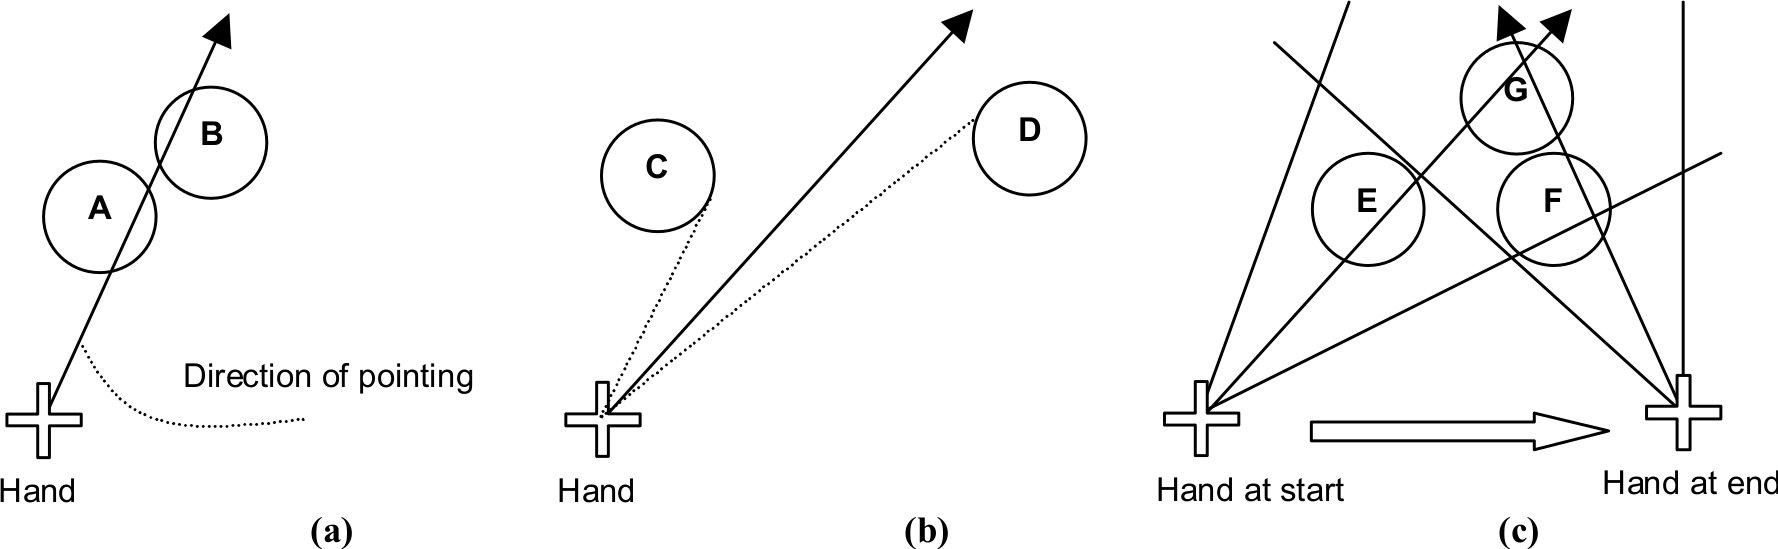
\includegraphics[width=0.9\textwidth]{figures/ch2/shadow}
		\caption[Fonctionnement du \emph{Shadow Cone}]{\emph{Shadow Cone}. (a) Sélection par \emph{raycasting} classique : le premier objet croisé par le rayon est sélectionné (A ici). (b) Sélection par cône : l'objet le plus proche de l'axe de révolution du cône est sélectionné (D ici). (c) \emph{Shadow Cone} : l'objet sélectionné est celui qui est inclus dans le cône de sélection à tous les instants entre la pression du bouton du périphérique et son relâchement (G ici). Crédit : \cite{steed20043d}.}
		\label{fig:shadow}
	\end{figure}
	
	\paragraph{Performances.}
	Steed et Parker ont évalué les temps de sélection du \emph{Shadow Cone}, comparé à la sélection par rayon ou par cône.

	\begin{figure}[!htb]
		\begin{subfigure}[t]{0.49\textwidth}
			\centering
			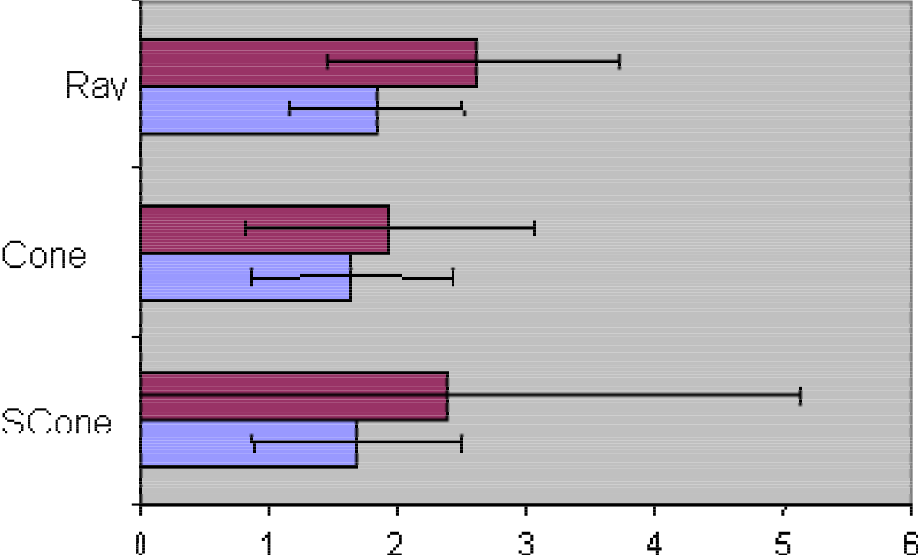
\includegraphics[width=\textwidth]{figures/ch2/shadowSLarge}
			\caption{Performances du \emph{Shadow Cone} (\emph{SCone}) avec une grande cible, comparé à la sélection par rayon et par cône. Chaque technique est évaluée avec suivi de la tête (en bleu) et sans (en violet). Le \emph{Shadow Cone} ne peut se distinguer de la sélection par rayon ou par cône, mais fournit des performances satisfaisantes.}
			\label{fig:shadowSLarge}
		\end{subfigure}
		~
		\begin{subfigure}[t]{0.49\textwidth}
			\centering
			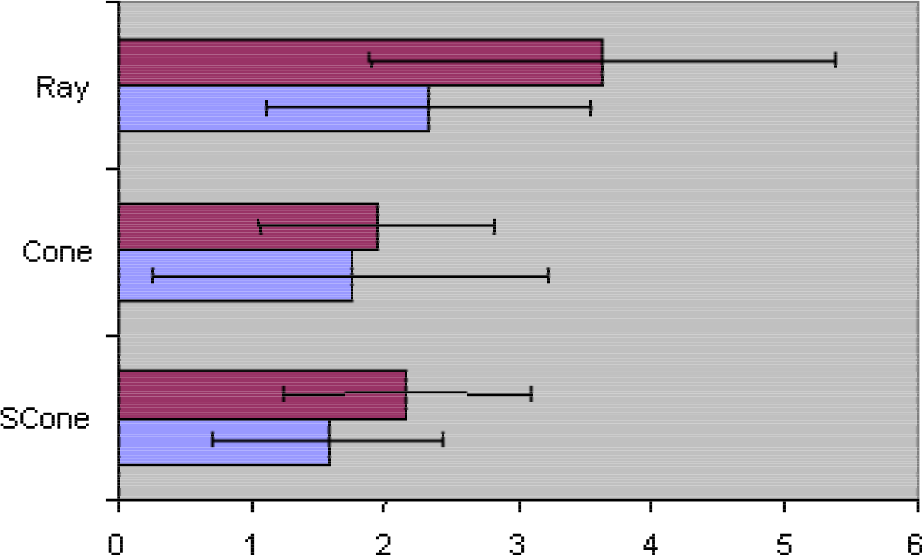
\includegraphics[width=\textwidth]{figures/ch2/shadowSSmall}
			\caption{Performances du \emph{Shadow Cone} avec une petite cible. Le \emph{Shadow Cone} ne peut se distnguer de la sélection par cône, mais ces deux techniques font bien mieux que la sélection par rayon.}
			\label{fig:shadowSSmall}
		\end{subfigure}
		\caption[Performances du \emph{Shadow Cone}]{Performances du \emph{Shadow Cone}. Crédit : \cite{steed20043d}.}
		\label{fig:shadowConePerf}
	\end{figure}
	
	Les temps de sélection mesurés pour les différentes techniques, avec et sans suivi de la tête, sont présentés sur la figure~\ref{fig:shadowSLarge} pour une grande cible seule, la figure~\ref{fig:shadowSSmall} pour une petite cible seule, la figure~\ref{fig:shadowPLarge} pour une grande cible avec un distracteur, la figure~\ref{fig:shadowPSmall} pour une petite cible avec un distracteur, la figure~\ref{fig:shadowCLarge} pour une grande cible avec de nombreux distracteurs, et enfin la figure~\ref{fig:shadowCSmall} pour une petite cible avec de nombreux distracteurs.
	
	Quoique les figures sus-citées présentent les résultats avec et sans suivi de la tête, nous nous contenterons ici de commenter les résultats avec suivi, attendu que le cas particulier de rendu immersif incorrect dans un SID dépasse le cadre de cet état de l'art, et n'est pas particulièrement pertinent au regard des besoins et applications identifiés au cour du premier chapitre. Observons simplement que, pour une condition et une technique données, le suivi de la tête améliore toujours les temps de sélection, comme l'on pouvait s'y attendre ; l'effet sur les erreurs et échecs est généralement le même.

	\begin{figure}[!htb]
		\begin{subfigure}[t]{0.49\textwidth}
			\centering
			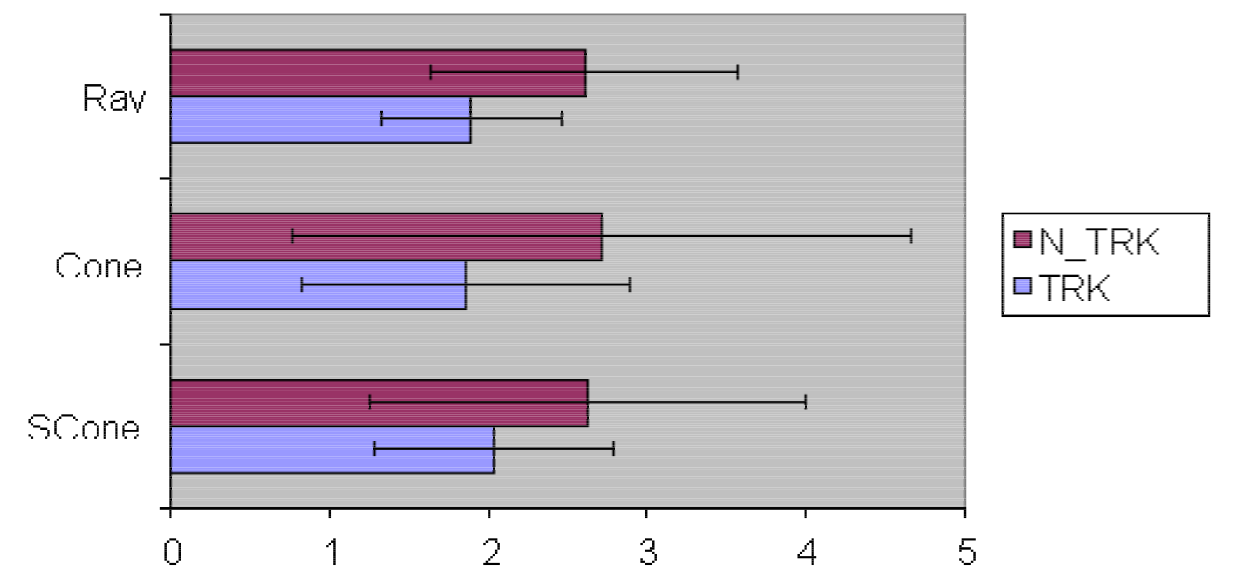
\includegraphics[width=\textwidth]{figures/ch2/shadowPLarge}
			\caption{Performances du \emph{Shadow Cone} avec une paire de grands objets. Aucune différence significative n'est mesurable entre les techniques pour les temps de sélection, mais le \emph{raycasting} ne produisit aucune erreur, contre 1,3 erreur par utilisateur pour la sélection par cône et 0,2 pour le \emph{Shadow Cone}, avec suivi de la tête dans les deux cas.}
			\label{fig:shadowPLarge}
		\end{subfigure}
		~
		\begin{subfigure}[t]{0.49\textwidth}
			\centering
			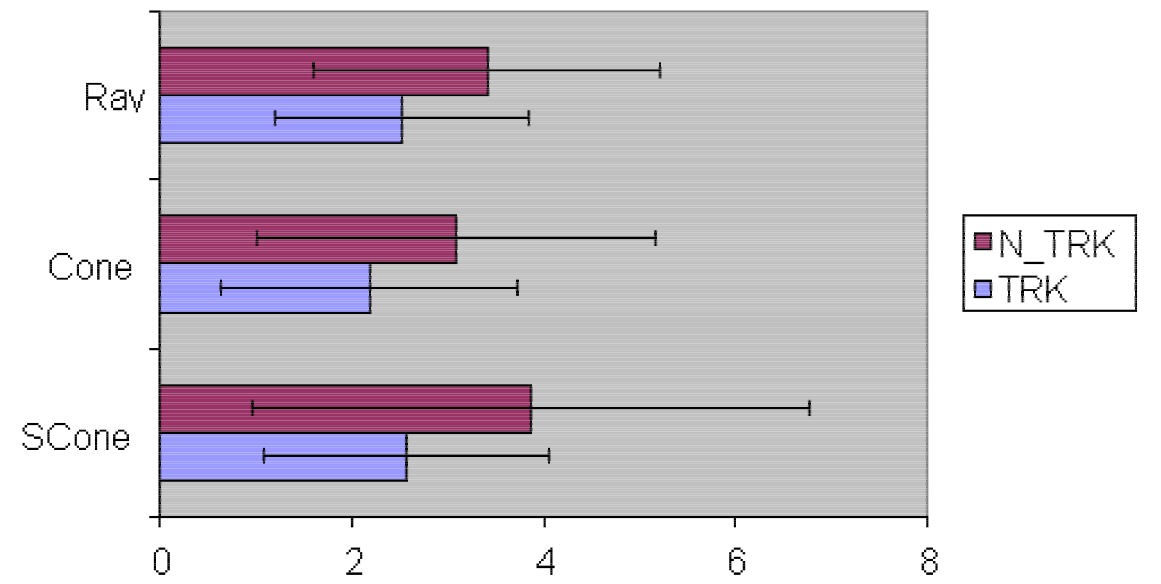
\includegraphics[width=\textwidth]{figures/ch2/shadowPSmall}
			\caption{Performances du \emph{Shadow Cone} avec une paire de petits objets. Le \emph{Shadow Cone} est ici plus lent que la sélection par cône, mais génère moins d'erreurs (0,2 par utilisateur contre 0,6) ; la sélection par rayon ne produisit aucune erreur, là encore avec suivi de la tête.}
			\label{fig:shadowPSmall}
		\end{subfigure}
		\caption[Performances du \emph{Shadow Cone} -- II]{Performances du \emph{Shadow Cone} -- II. Crédit : \cite{steed20043d}.}
		\label{fig:shadowConePerf2}
	\end{figure}

		
	\begin{figure}[!htb]
		\begin{subfigure}[t]{0.49\textwidth}
			\centering
			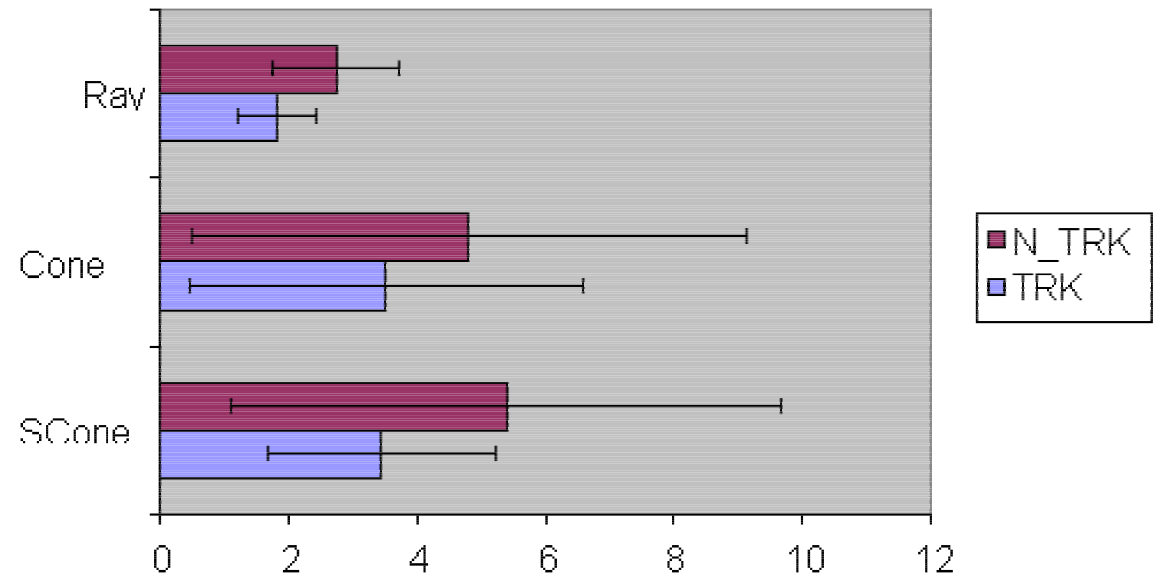
\includegraphics[width=\textwidth]{figures/ch2/shadowCLarge}
			\caption{Performances du \emph{Shadow Cone} avec une grappe de gros objets. Ici, c'est le \emph{raycasting} qui se montre nettement plus performant que les autres techniques. La sélection par cône a en outre généré 2,2 échecs par \emph{timeout} par utilisateur, alors que les deux autres techniques n'en ont généré aucun (avec suivi de la tête). De plus, la sélection par cône généra 20,3 erreurs par utilisateur, contre 5,2 pour le \emph{Shadow Cone} et 0,5 pour le \emph{raycasting}.}
			\label{fig:shadowCLarge}
		\end{subfigure}
		~
		\begin{subfigure}[t]{0.49\textwidth}
			\centering
			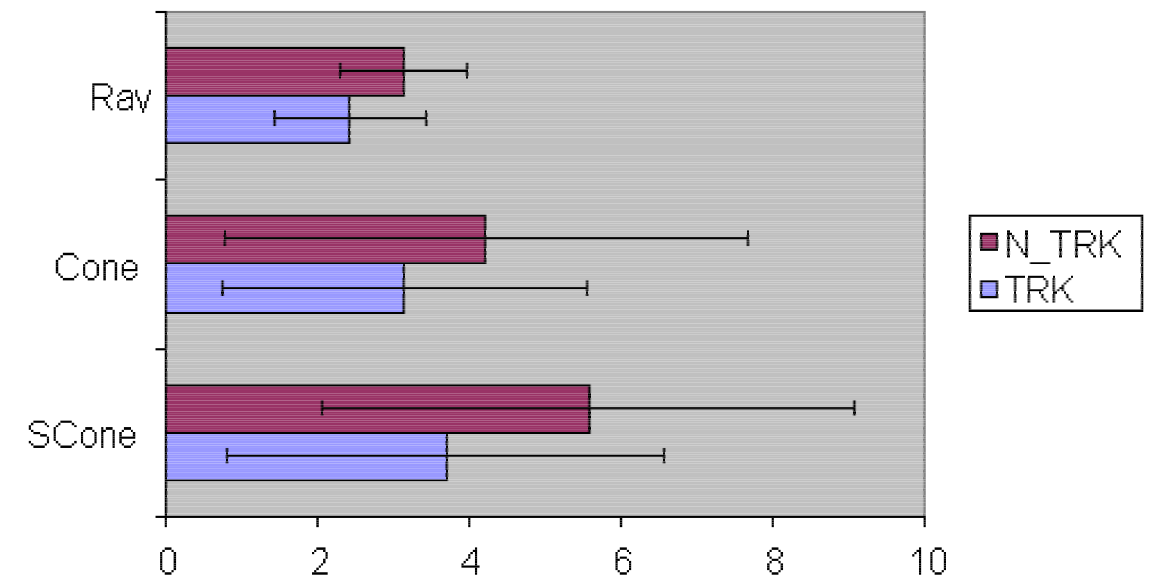
\includegraphics[width=\textwidth]{figures/ch2/shadowCSmall}
			\caption{Performances du \emph{Shadow Cone} avec une grappe de petits objets. Le \emph{raycasting} est le plus performant avec suivi de la tête. Dans cette condition, l'écart entre les autres techniques n'est pas significatif. La sélection par cône généra 2 échecs par \emph{timeout} par utilisateur, contre aucun pour les autres techniques, avec suivi de la tête. Le \emph{Shadow Cone} a un taux d'erreurs élevé : 4,5 par utilisateur, contre 4,4 pour la sélection par cône et 1,2 pour le \emph{raycasting}, avec suivi de la tête.}
			\label{fig:shadowCSmall}
		\end{subfigure}
		\caption[Performances du \emph{Shadow Cone} -- III]{Performances du \emph{Shadow Cone} -- III. Crédit : \cite{steed20043d}.}
		\label{fig:shadowConePerf3}
	\end{figure}
	
	\subsubsection{Le problème de l'ambiguïté en environnement dense}
	Lorsque l'environnement est particulièrement dense, la sélection par rayon ou cône devient difficile~\cite{kopper2011rapid}, car la précision requise devient très élevée, tant pour l'utilisateur que pour le système de suivi du périphérique de pointage. L'utilisation d'un cône facilite la sélection de petites cibles, mais ajoute un risque d'ambiguïté. Une solution pourrait être d'augmenter le ratio contrôle/affichage à proximité des cibles~\cite{frees2007prism, kopper2010human}, mais c'est au prix de l'introduction d'un décalage entre l'orientation réelle du périphérique de pointage et celle du rayon qu'il lance, ce qui peut être très troublant, et ingérable avec des cibles mobiles, surtout rapides.
	
	Et si diverses techniques peuvent aider à lever l'ambiguïté, leur utilisation est d'autant plus difficile que les cibles situées dans le volume du cône sont nombreuses, petites et\ldots{} mobiles. En effet, la mobilité des cibles nécessite d'effectuer des mouvements plus rapides pour les pointer, donc d'exercer plus de force, et de fait, d'être moins précis~\cite{schmidt1979motor}. En particulier, le \emph{Shadow Cone} impose de maintenir la cible visée à l'intérieur du cône pendant toute la phase de désambiguïsation, ce qui peut s'avérer extrêmement difficile avec une cible en mouvement, \emph{a fortiori} si ses mouvements sont rapides et/ou imprévisibles. Par conséquent, nous ne pouvons retenir cette technique pour les applications qui nous intéressent.
	
	Néanmoins, observons qu'en assouplissant quelque peu cette contrainte, le \emph{Shadow Cone} fournirait potentiellement de meilleurs résultats avec les cibles mobiles. C'est en substance ce que propose le \emph{Smart Ray}~\cite{grossman2006design}, décrit plus bas.

	\subsection{\emph{Raycasting} avec désambiguïsation}
	Dans~\cite{grossman2006design}, Grossman \emph{et al.} proposent d'évaluer diverses techniques de sélection dérivées du \emph{raycasting} et ayant pour but de faciliter la désambiguïsation lorsque le rayon atteint plusieurs objets. Ces travaux sont présentés comme étant motivés par l'émergence d'écrans volumétriques~\cite{ebert1999realizing}, mais demeurent très pertinents pour des dispositifs d'affichage plus classiques, notamment stéréoscopiques.

	\subsubsection{\emph{Depth Ray}}
	Le \emph{Depth Ray}~\cite{grossman2006design} fonctionne comme une technique de \emph{raycasting} traditionnelle, si ce n'est que la position du périphérique de pointage le long de son axe est prise en compte, comme le montre la figure~\ref{fig:depthRay}. Le rayon est augmenté d'un marqueur de profondeur que l'utilisateur déplace le long du rayon simplement en avançant ou en reculant le périphérique de pointage.
	
	\newcommand{\rayWidth}{0.55\textwidth}
	\begin{figure}[!htb]
		\centering
		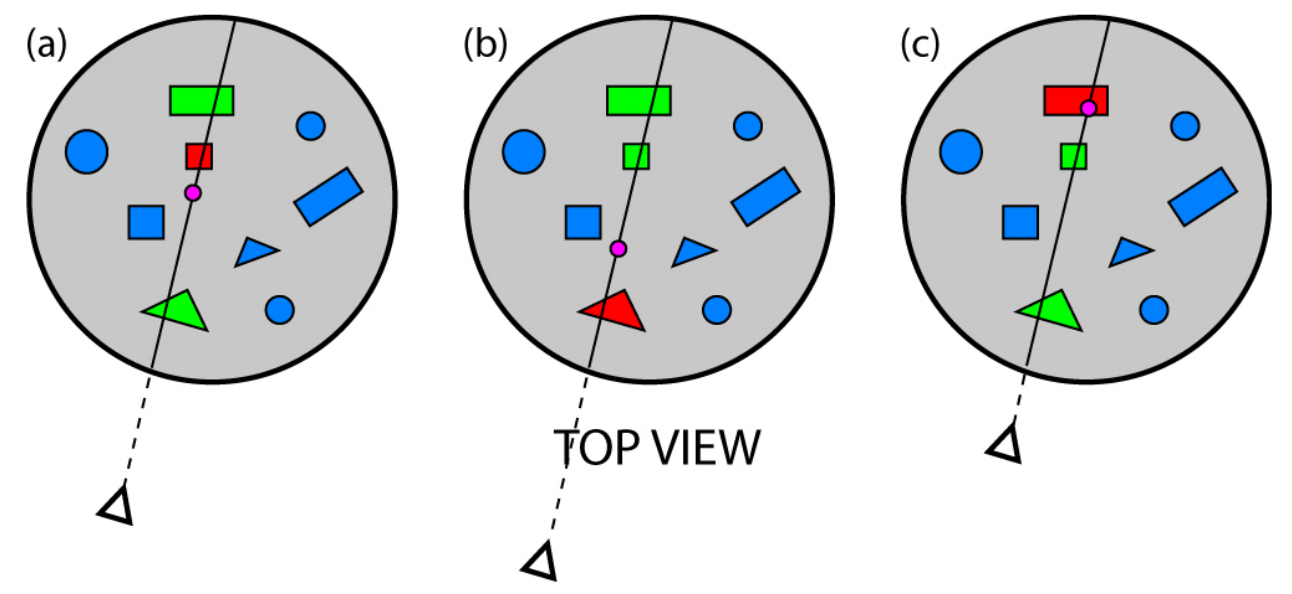
\includegraphics[width=\rayWidth]{figures/ch2/depthRay}
		\caption[Principe du \emph{Depth Ray}]{Fonctionnement du \emph{Depth Ray}. (a) Un marqueur rose est utilisé pour sélectionner la cible intersectée la plus proche de lui --- notons que le marqueur fonctionne par proximité et n'a pas besoin d'être \emph{sur} la cible. (b) Reculer le périphérique de pointage recule le marqueur et permet de séletionner une cible plus proche. (c) Inversement, avancer le périphérique permet d'avancer le marqueur et de sélectionner une cible plus lointaine. Crédit : \cite{grossman2006design}.}
		\label{fig:depthRay}
	\end{figure}
	
	\subsubsection{\emph{Lock Ray}}
	Le \emph{Lock Ray}~\cite{grossman2006design} fonctionne de la même façon que le \emph{Depth Ray}, si ce n'est qu'une fois que le rayon est positionné, il est \emph{verrouillé} --- d'où le nom --- afin de permettre à l'utilisateur de déplacer le marqueur de profondeur sans avoir à craindre de faire bouger le rayon par accident.
	
	\begin{figure}[!htb]
		\centering
		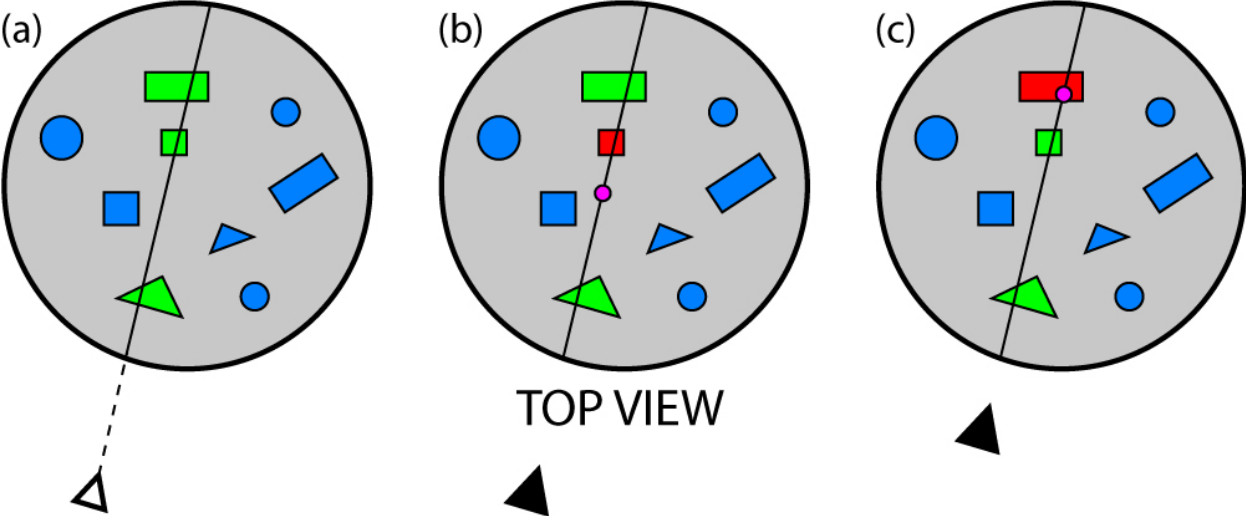
\includegraphics[width=\rayWidth]{figures/ch2/lockRay}
		\caption[Principe du \emph{Lock Ray}]{Fonctionnement du \emph{Lock Ray}. (a) La sélection commence par une phase de \emph{raycasting} classique, sans marqueur de profondeur. (b) Une fois que l'utilisateur a pressé le bouton du périphérique un marqueur de profondeur apparaît au milieu du segmet du rayon inclus dans la sphère. (c) L'utilisateur peut déplacer le marqueur en déplaçant sa main, comme dans le \emph{Depth Ray}, et effectue la sélection en relâchant le bouton. Crédit : \cite{grossman2006design}.}
		\label{fig:lockRay}
	\end{figure}
	
	\subsubsection{\emph{Flower Ray}}
	Comme le \emph{Lock Ray}, le \emph{Flower Ray}~\cite{grossman2006design} fonctionne avec deux phases distinctes. Dans la première, l'utilisateur place son rayon dans la position et l'orientation qu'il désire ; puis, il le fixe, et les objets croisés par le rayon \og s'épanouissent \fg{}  --- tout autour d'un curseur ponctuel, comme les pétales d'une fleur autour de son pistil, ainsi que l'illustre la figure~\ref{fig:flowerRay}. Dans le menu \og floral \fg{} les objets sont disposés par ordre de profondeur croissante dans le sens horaire, avec le plus proche en haut à droite.
	
	\begin{figure}[!htb]
		\centering
		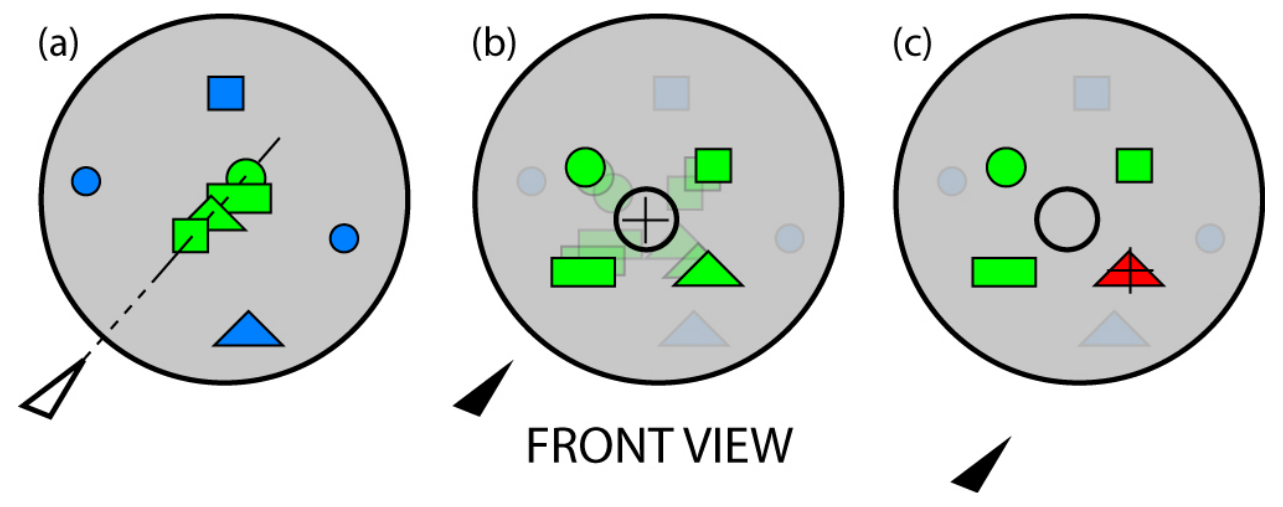
\includegraphics[width=\rayWidth]{figures/ch2/flowerRay}
		\caption[Principe du \emph{Flower Ray}]{Fonctionnement du \emph{Depth Ray}. (a) Toutes les cibles croisées par le rayon sont colorées en vert. (b) Quand l'utilisateur presse le bouton de son périphérique, ces objets s'épanouissent en un menu de sélection autour d'un curseur poncuel, qui apparaît à cet instant. (c) L'utilisateur peut à présent pointer près de la cible et relâcher le bouton pour la sélectionner. Crédit : \cite{grossman2006design}.}
		\label{fig:flowerRay}
	\end{figure}
	
	\subsubsection{\emph{Smart Ray}}
	Par définition, un rayon contient une infinité de points. Toutefois, si deux sont sécants, alors ils n'ont qu'un seul point en commun. Il donc possible d'utilier deux rayons pour effectuer une sélection par \emph{raycasting} sans aucune ambiguïté. Toutefois, cela nécessite deux périphériques de saisie et cela occupe les deux mains de l'utilisateur.
	
	Le \emph{Smart Ray}~\cite{grossman2006design} propose donc de faire cela avec deux rayons issus du même périphérique, mais mesurés à deux instant différents, selon un principe proche de celui du \emph{Shadow Cone}~\cite{steed20043d}. Chaque objet se voit attribuer un \og poids \fg{} qui croît d'autant plus que le rayon est proche de son centre, ou décroît d'autant plus qu'il en est loin, continuellement. L'objet dont le poids est le plus élevé peut être sélectionné, comme l'illustre la figure~\ref{fig:smartRay}.
	
	\begin{figure}[!htb]
		\centering
		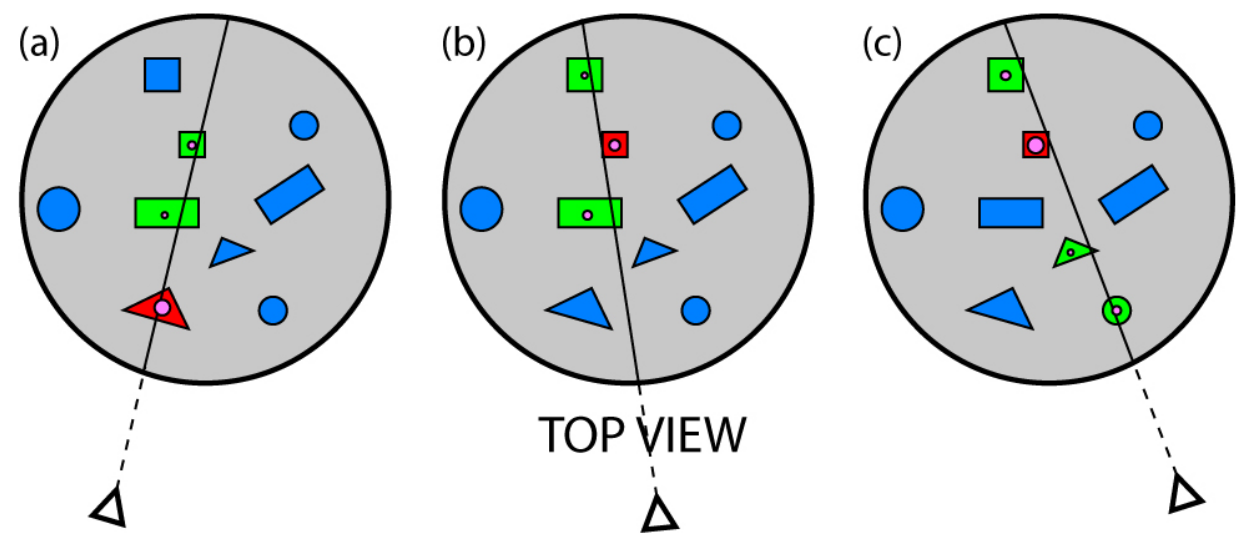
\includegraphics[width=\rayWidth]{figures/ch2/smartRay}
		\caption[Principe du \emph{Smart Ray}]{Utilisation du \emph{Smart Ray} pour sélectionner le petit carré. (a) Les poids des cibles sont basés sur la distance entre le rayon et la cible, et visualisés par de petites sphères au centre de chaque cible. À tout moment, la cible avec le plus gros poids peut être sélectionnée. (b,c) Le rayon peut être repositionné en continu pour augmenter le poids de la cible visée, même si elle est occultée. Crédit : \cite{grossman2006design}.}
		\label{fig:smartRay}
	\end{figure}
	
	\subsubsection{Motivations}
	Grossman \emph{et al.}~\cite{grossman2006design} notent que les techniques présentées ci-dessus ont chacune des avantages et des inconvénients. Le \emph{Depth Ray} unifie les phases de sélection et de désambiguïsation, ce qui peut faire gagner du temps mais aussi causer des perturbations entre les phases. Le \emph{Lock Ray} sépare les phases explicitement, mais désambiguïse avec un menu linéaire. Le \emph{Flower Ray} propose un menu radial, théoriquement plus rapide, mais les utilisateurs doivent suivre l'animation pour ne pas perdre leur cible entre les deux phases. Enfin, le \emph{Smart Ray} fournit un mode de désambiguïsation implicite et possiblement plus fluide, mais potentiellement source de frustration s'il échoue à prédire correctement l'intention de l'utilisateur, comme toujours avec les techniques prédictives.
	
	\subsubsection{Évaluations}
	Avec ces mérites respectifs en tête, Grossman \emph{et al.} ont évalué ces quatre techniques dans un environnement dense, afin de rendre la désambiguïsation absolument nécessaire. De fait, la sélection par \emph{raycasting} classique est impossible, et donc ne fut pas évaluée ici. La technique de base considérée est donc le curseur ponctuel.

	\paragraph{Temps de sélection.}
	
	Les temps de sélection mesurés par les auteurs pour les différentes techniques sont représentés sur la figure~\ref{fig:rayTimes}.
	
	\begin{figure}[!htb]
		\begin{subfigure}[t]{0.49\textwidth}
			\centering
			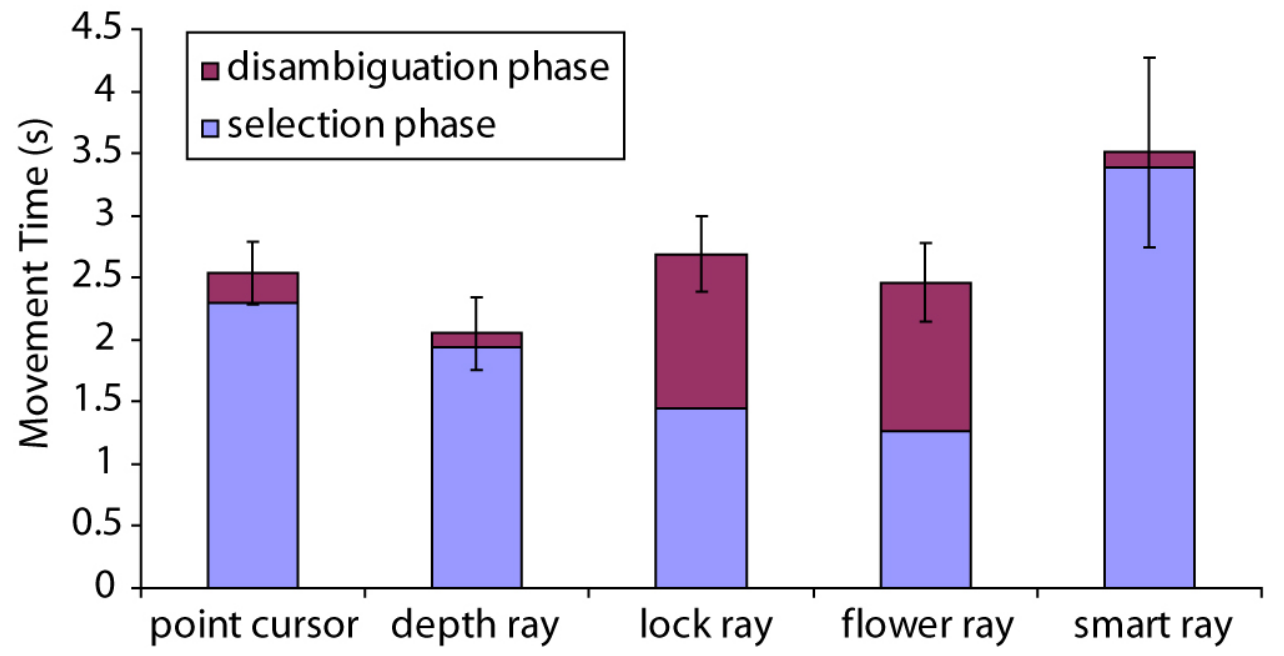
\includegraphics[width=\textwidth]{figures/ch2/rayTimes}
			\caption{Évaluation des techniques de \emph{raycasting} avec désambiguïsation en environnement dense. Les résultats présentés sont les temps de sélection. Seul le \emph{Depth Ray} se montre plus performant que le curseur ponctuel.}
			\label{fig:rayTimes}
		\end{subfigure}
		~
		\begin{subfigure}[t]{0.49\textwidth}
			\centering
			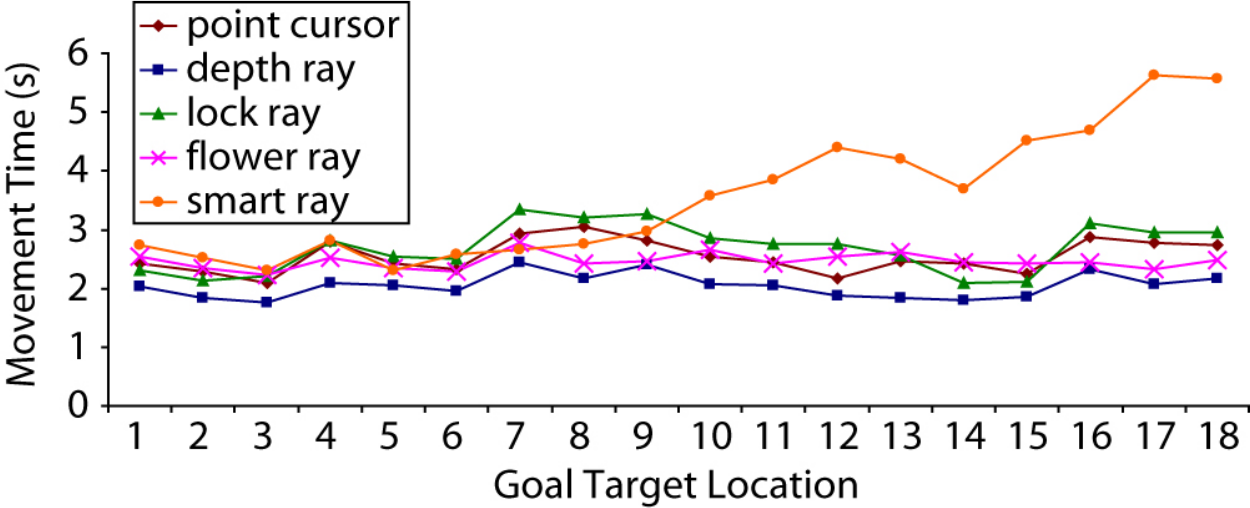
\includegraphics[width=\textwidth]{figures/ch2/smartRayLocation}
			\caption{Pour les cibles dont les identifiants sont faibles (vers la gauche) le \emph{Smart Ray} fournit de bons résultats, mais ils sont mauvais pour les cibles d'identifiant élevé (à droite). Tous les sujets de l'évaluation étaient droitiers, donc le rayon venait également de la droite, et rencontrait beaucoup d'obstacles.}
			\label{fig:smartRayLocation}
		\end{subfigure}
		\caption[Performances du \emph{raycasting} avec désambiguïsation]{Performances du \emph{raycasting} avec désambiguïsation. Crédit : \cite{grossman2006design}.}
		\label{fig:rayPerf}
	\end{figure}

	Le premier constat est que le curseur ponctuel offre de très bonnes performances par rapport aux techniques de \emph{raycasting}, ce qui peut surprendre compte tenu des performances généralement supérieures de ces dernières~\cite{bowman2001testbed}. Mais le niveau d'occultation avec de nombreux distracteurs est tel que les performances de cette classe de techniques chutent. Toutefois, le \emph{Depth Ray} fournit de très bons résultats, meilleurs que ceux du curseur ponctuel. Il profite selon toute probabilité de l'intégration des phases de sélection et de désambiguïsation. Grossman \emph{et al.} remarquent au passage que le temps de désambiguïsation du \emph{Flower Ray} est relativement constant en fonction de l'emplacement de la cible, alors que celui du \emph{Lock Ray} varie beaucoup ; sans doute le menu radial du premier a-t-il un effet lisseur sur cette valeur.

	\paragraph{Performances selon l'emplacement de la cible.}
	Les performances du \emph{Smart Ray} paraissent décevantes. Un examen plus poussé des résultats montre toutefois une forte interaction entre le temps de sélection et l'emplacement de la cible avec cette technique (voir la figure~\ref{fig:smartRayLocation}). Pour les cibles situées à droite, les performances s'effondrent, car le rayon part également de la droite (tous les sujets étant droitiers) donc rencontre beaucoup d'obstacles. Dans ces conditions, l'heuristique de prédiction du \emph{Smart Ray} échoue plus souvent.

	Ces mauvais résultats du \emph{Smart Ray} sont toutefois à nuancer, puisque les sujets avaient pour instruction de ne pas bouger leurs pieds ; s'ils avaient pu se déplacer, les résultats auraient probablement été meilleurs, à condition que leur temps de déplacement ne soit pas assez long pour annuler le bénéfice du déplacement.
	
	\paragraph{Distance parcourue par le périphérique.}
	Les auteurs ont par ailleurs mesuré la distance parcourue par le périphérique de pointage au cours d'une tâche de sélection, pour chaque technique évaluée. C'est un résultat important car il est déterminant pour la fatigue ressentie par un utilisateur sur une durée significative. Ici encore, le \emph{Smart Ray} déçoit, tandis que les autres techniques permettent de réduire la distance à parcourir par rapport au curseur ponctuel, comme l'illustre la figure~\ref{fig:rayFootprint}.
	
	\begin{wrapfigure}{O}{0.5\textwidth} % Capital O makes the figure float, because that's totally intuitive and obvious.
		\centering
		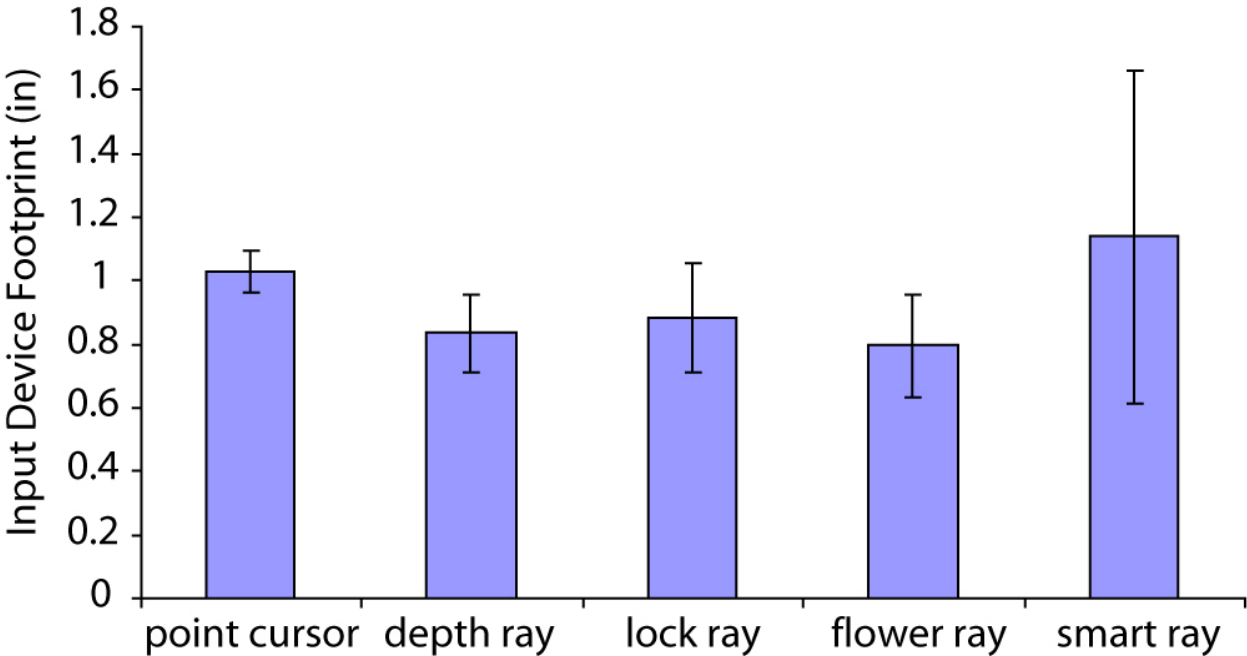
\includegraphics[width=0.46\textwidth]{figures/ch2/rayFootprint}
		\caption[\emph{Raycasting} et désambiguïsation -- distance parcourue par le périphérique]{Distance parcourue par le périphérique de pointage avec les diverses techniques de \emph{raycasting} évaluées. Les \emph{Depth, Lock} et\emph{Flower Rays} font mieux que le curseur ponctuel, au contraire du \emph{Smart Ray} qui affiche en outre un écart-type considérable. Crédit : \cite{grossman2006design}.}
		\label{fig:rayFootprint}
	\end{wrapfigure}
	
	Là encore on peut s'interroger sur la solidité des distances mesurées sur \emph{Smart Ray} attendu que dans un contexte \og réel \fg{} les utilisateurs seraient libres de se déplacer. Naturellement, la quantité de mouvement absolue du pointeur pourrait s'en trouver accrue, mais sa quantité de mouvement relatif à l'utilisateur pourrait diminuer. Il resterait à déterminer s'il est plus fatigant de bouger beaucoup son bras, ou un peu son corps et un peu son bras. Cette question est à notre connaissance ouverte.
	
	\paragraph{Taux d'erreurs.}
	Enfin, Grossman \emph{et al.} rapportent que les taux d'erreurs sont avantageux avec ces techniques de \emph{raycasting} avec désambiguïsation, comme le détaille la table~\ref{tab:rayErrors}.
	
%	\newcommand{\newrow}{\bigstrut[t] \\ \hline}
	\begin{table}
	\centering
	\begin{tabular}{c c}
		Type de curseur			& Taux d'erreurs \bigstrut[b] \\ \hline
		Curseur ponctuel		& 20,7~\%{} \bigstrut[t] \\
		\emph{Depth Ray}		& 13,3~\%{} \\
		\emph{Lock Ray}			& 11,1~\%{} \\
		\emph{Flower Ray}		& 10,9~\%{} \\
		\emph{Smart Ray}		& 10,4~\%{} \\
	\end{tabular}
	\caption[Taux d'erreurs pour les techniques de \emph{raycasting} avec désambiguïsation]{Taux d'erreurs pour les techniques de \emph{raycasting} avec désambiguïsation. Données tirées de~\cite{grossman2006design}.}
	\label{tab:rayErrors}
	\end{table}
	
	\subsubsection{Conclusion}
	L'étude de Grossman \emph{et al.}~\cite{grossman2006design} montre qu'en environnement dense, la sélection par \emph{raycasting} pur est moins efficace qu'un curseur ponctuel, voire impossible, mais que des méthodes de désambiguïsation peuvent permettre d'atteindre de meilleures performances. Dans une certaine mesure, on peut en effet améliorer les temps de sélection, mais les bénéfices sur les taux d'erreurs sont encore plus importants.
	
	Parmi les techniques évaluées ici, le \emph{Depth Ray} se distingue des autres avec de très bons temps de sélection, et un taux d'erreurs plus élevé que ceux des autres techniques avancées, mais tout de même nettement inférieur à ce qu'on obtient avec un curseur ponctuel. Toutefois, le \emph{Depth Ray} souffre d'un léger inconvénient, puisqu'il nécessite un périphérique de pointage permettant de capturer non seulement son orientation, mais également sa position. Ce n'est pas nécessairement le cas du \emph{Lock Ray} ou du \emph{Flower Ray}, par exemple.
	
	Ce qui est potentiellement plus gênant avec le \emph{Depth Ray} est le couplage des phases de pré-sélection et de désambiguïsation. Si ce couplage est bénéfique ici, on peut en douter dans le cas de cibles mobiles, où il faudrait constamment réajuster l'orientation du rayon pour continuer à \og capturer \fg{} la cible, tout en avançant ou reculant le périphérique pour placer le marqueur de profondeur au bon endroit. Nous supposons que pour des cibles petites et/ou rapides, le \emph{Depth Ray} serait très difficile à utiliser, là où un \emph{Lock/Flower Ray} pourrait fournir des performances satisfaisantes, à condition peut-être d'utiliser un cône un peu large au lieu d'un rayon cylindrique --- en réalité, ces techniques furent mises en \oe{}uvre par Grossman \emph{et al.} avec des cônes de 2\textdegree{} d'angle, même si ce n'était pas indiqué par le rendu graphique.
	
	Si le \emph{Smart Ray} fournit ici d'assez mauvais résultats, il serait intéressant de le réévaluer dans ce contexte, car d'une part, il souffrirait peut-être moins de l'occultation de la cible si elle était mobile, et d'autre part, il ne serait peut-être plus nécessaire de bouger le rayon pour lever l'ambiguïté, puisqu'en suivant la cible, son poids augmenterait continuellement, tandis que les poids des distracteurs seraient susceptibles de baisser assez rapidement --- à moins que ceux-ci ne se déplacent de façon corrélée à la cible, en étant toujours touchés par le rayon, ce qui est assez improbable sur une durée de plusieurs secondes dans la plupart des cas.
	
	Ainsi, les inconvénients principaux de cette technique, à savoir la distance parcourue par le périphérique et l'occultation pourraient être atténués, tandis que l'heuristique de prédiction pourrait \emph{mieux} fonctionner qu'avec des cibles statiques. Nous verrons plus loin que la technique \emph{IntenSelect}~\cite{de2005intenselect} fonctionne à peu près sur ce principe, de même que \emph{Hook}~\cite{ortega2013hook}, qui fait cependant usage d'un curseur ponctuel.

	\subsection{Sélection en cascade, grossière, puis fine}
	Les techniques de cette catégorie divisent la sélection en deux phases (ou plus). Premièrement, une portion de l'espace visuel est sélectionnée. Cette première phase étant grossière, elle n'a pas besoin d'être précise, et peut être très rapide. Par exemple, avec un simple périphérique de pointage, tel qu'une souris, un ratio contrôle/affichage (\emph{control/display, C/D}) très faible peut être utilisé. Le curseur (ou autre medium de sélection) peut ainsi se placer très rapidement sur la zone d'intérêt, mais n'a pas besoin d'être précisément sur la cible pour délencher la deuxième phase : la sélection (plus) fine. Dans celle-ci, l'utilisateur sélectionne la cible elle-même, par exemple à l'aide d'un ratio C/D plus élevé, ou bien affine encore l'espace de sélection, jusqu'à ce qu'une phase finale permette la sélection effective de la cible.
	 
	Du point de vue de la loi de Fitts, au cours d'une phase grossière, la cible bénéficie d'une largeur accrue (car c'est toute une zone autour de la cible qui est visée) tandis que la phase finale offre une distance réduite, puisque le curseur se trouve déjà près de la cible. Quoiqu'il y ait probablement un certain \og coût cognitif \fg{} lié au basculement d'une phase à l'autre, et en tout cas un coût temporel associé à la pression d'un bouton ou à toute autre action permettant de passer à la phase suivante, les techniques de sélection en cascade peuvent améliorer significativement les performances de sélection, même pour les tâches dont l'indice de difficulté est élevé~\cite{kopper2011rapid}.
	
	La sélection en cascade revient, en substance, à préférer une série de tâches très rapides et faciles à une seule tâche nécessitant une précision élevée, prenant du temps et pouvant être source d'erreur plus ou moins fréquentes. Observons que la sélection en cascade, du fait de la réduction du taux d'erreurs qu'elle permet, présente un intérêt particulier pour les tâches critiques, celles pour lesquelles une erreur peut avoir des conséquences graves.
	
	\subsubsection{Utilisation du regard}
	Une estimation de la direction du regard de l'utilisateur peut être utilisée soit pour sélectionner directement la cible (ce qui peut nécessiter beaucoup de précision, quand la cible est petite) soit pour sélectionner une zone d'intérêt, dans la phase grossière d'une sélection en cascade. C'est généralement dans cette seconde fonction que l'on trouve cette technique, selon le principe \og le regard suggère, le toucher confirme \fg{}~\cite{stellmach2012look}.

	L'estimation de la direction du regard d'autrui faite par un individu est basée sur la combinaison de la position de la tête de la personne observée, de l'orientation de sa tête, et de l'orientation de ses yeux~\cite{langton2004influence}, mais elle est fortement biaisée par l'orientation de la tête~\cite{wollaston1824apparent}.
	
	Sur l'hypothèse que l'estimation de la direction du regard faite instinctivement par les êtres humains se base sur une méthode efficace, on peut en déduire qu'une méthode artificielle devrait procéder de la même façon, c'est-à-dire en estimant la position et la direction de la tête d'une part, et la direction des yeux de l'autre. Murphy Chutorian et Trivedi~\cite{murphy2009head} proposent une taxinomie et un inventaire détaillés des techniques d'estimation de la \emph{pose}\footnote{C'est-à-dire de la position \emph{et} de l'orientation.} de la tête. Ces techniques sont toutefois destinées à traiter des données vidéo brutes.
	
	Or, dans le cas qui nous intéressent, il est généralement possible d'installer des marqueurs sur la tête d'un utilisateur pour connaître plus précisément sa \emph{pose}, en s'appuyant également sur des caméras de \emph{tracking}, comme par exemple les systèmes d'Advanced Realtime Tracking\footnotemark{}. Outre sa précision, ce système est autrement plus robuste que les techniques sans marqueurs.
	
	\footnotetext{Des réseaux de caméras infrarouge permettant d'obtenir les positions précises d'un ensemble de marqueurs, donc l'orientation de l'objet sur lequel les marqueurs sont posés --- objet pouvant éventuellement être la tête d'un utilisateur.
	\url{http://www.ar-tracking.com/products/tracking-systems/arttrack-system/arttrack5}}
	
	Comme le rappellent Zhai \emph{et al.}~\cite{zhai1999manual}, l'utilisation des yeux comme entrée dans un système informatique fait l'objet de recherches depuis longtemps~\cite{levine1981eye, bolt1982eyes, ware1987evaluation, jacob1990you}. Ils remarquent également que la fovéa, (la zone centrale de la macula, la zone de la rétine où la vision des détails est la plus précise) avec son angle de 1\textdegree{}, est trop grossière pour les cibles les plus petites, surtout compte tenu des mouvements aléatoire constamment effectués par les yeux~\cite{monden2005evaluation, vspakov2011comparison}. Dans uen certaine mesure, ces derniers peuvent être filtrés, mais cela ne règle que partiellement le problème~\cite{zhang2008improving}.
	
	Par ailleurs, il peut être très déroutant pour un utilisateur de \og charger \fg{} un canal sensoriel, habituellement passif\footnotemark{}, d'une fonction de manipulation plus généralement dévolue à une extrémité ou un membre.
	
	\footnotetext{Remarquons cependant que le regard, quand il est contrôlé de façon délibérée, peut être utilisé pour communiquer, par exemple lorsqu'une personne en invite une autre, oralement, à regarder quelque chose qu'elle désigne du regard. Lever les yeux au ciel peut communiquer de l'agacement ou du dédain, etc.}
	
	Dès lors, il serait tentant de rejeter cette technique, et \emph{a fortiori} l'estimation de la \emph{pose} de la tête ne tenant pas compte des yeux, puisque c'est forcément beaucoup moins précis. Mais ce serait faire fi un peu trop rapidement des avantages du suivi des yeux, et en particulier de sa rapidité inégalée. Certes, il ne peut suffire à lui seul à sélectionner un objet d'indice de difficulté élevé ; il n'est pas inutile pour autant, loin s'en faut.

	En effet, des études ont en effet montré que le regard permettait de faire mieux que les périphériques de saisie traditionnels pour des tâches de sélection~\cite{stellmach2012look, ware1987evaluation, smith2000hand, bieg2010eye}.
	
	\paragraph{Suivi des yeux : une tâche ardue.}

	Cependant, le suivi des yeux présente en pratique des difficultés qui peuvent être considérables, dont au moins les suivantes :
	
	\begin{itemize}
		\item Les performances peuvent dépendre de la couleur des yeux ;
		\item Le suivi des yeux ne fonctionne pas toujours bien en environnement sombre, par exemple dans un CAVE ;
		\item Les lunettes peuvent nuire aux performances du système ;
		\item Les lunettes stéréoscopiques, en particulier, occultent partiellement les yeux pour les \emph{trackers} oculaires, et réduisent la luminosité du blanc des yeux.
	\end{itemize}

	Par conséquent, l'utilisation de suivi des yeux se montre souvent difficile à mettre en œuvre, quoique les progrès techniques puissent, dans un futur proche, pallier au moins partiellement ces difficultés.
	
	Du reste, même quand le suivi des yeux est impossible et seule la tête peut être pris en compte, les informations captées demeurent précieuses. En effet, 40~\%{} à 70~\%{} de l'orientation du regard est déterminée par la rotation de la tête, tandis que les 60~\%{} à 30~\%{} restants (respectivement) dépendent des mouvements oculaires~\cite{gauthier1991short}. On peut donc, le plus souvent, obtenir une bonne estimation de la direction du regard en se fondant uniquement sur l'orientation de la tête.
	
	\subsubsection{\emph{Look \&{} Touch}}
	Stellmach \emph{et al.}~\cite{stellmach2012look} ont développé et évalué plusieurs techniques fondées sur le principe de la sélection en cascade avec une phase grossière dirigée par le regard, et une phase fine s'appuyant sur un périphérique doté d'un écran tactile, tel qu'un \emph{smartphone}.
	
	\begin{enumerate}
		\item \textbf{\emph{Gaze-directed cursor} :} Ce mode très simple peut à peine être considéré comme une cascade : l'utilisateur suit sa cible des yeux, puis appuie sur un écran tactile et le relâche pour effectuer la sélection. Voir la figure~\ref{fig:lookandtouch}, à gauche.
		\item \textbf{\emph{MAGIC touch} absolue :} Cette technique est analogue à la précédente, mais le curseur peut être déplacé en fonction de la position absolue du doigt de l'utilisateur sur son écran tactile. Voir la figure~\ref{fig:lookandtouch}, deuxième vignette.
		\item \textbf{\emph{MAGIC touch} relative :} Cette technique est identique à la précédente, mais le curseur positionnement du curseur dépend des mouvements relatifs du doigt de l'utilisateur par rapport à son point de départ. Voir la figure~\ref{fig:lookandtouch}, troisième vignette.
		\item \textbf{\emph{MAGIC tab} :} Cette technique demeure similaire aux précédentes, mais le curseur ne bouge pas ; en revanche, l'utilisateur peut parcourir les objets comme dans un menu, en faisant glisser son doigt. Ce procédé s'inspire de la touche \emph{tabulation} d'un clavier. Voir la figure~\ref{fig:lookandtouch}, à droite.
		\item \textbf{\emph{Gaze-supported Expanded Target Selection} asservie au regard :} Le regard contrôle une lentille de zoom, inactive par défaut, mais activée en appuyant sur l'écran tactile. Une nouvelle pression permet de sélectionner la cible, tandis qu'un geste de glissement vertical permet d'ajuster le niveau de zoom. Cette technique est illustrée par la figure~\ref{fig:lookandtouch2}, à gauche et au milieu.
		\item \textbf{\emph{Gaze-supported Expanded Target Selection} semi-fixe :} Contrairement à la technique précédente, la lentille cesse de bouger une fois activée, et l'utilisateur déplace le curseur au sein de la zone de zoom à l'aide de son regard, avant d'activer la sélection avec son écran tactile. Si son regard quitte la zone de zoom, alors la lentille se déplace. Voir la figure~\ref{fig:lookandtouch2}, vignettes de gauche et de droite.
	\end{enumerate}
	
	\begin{figure}[!htb]
		\centering
		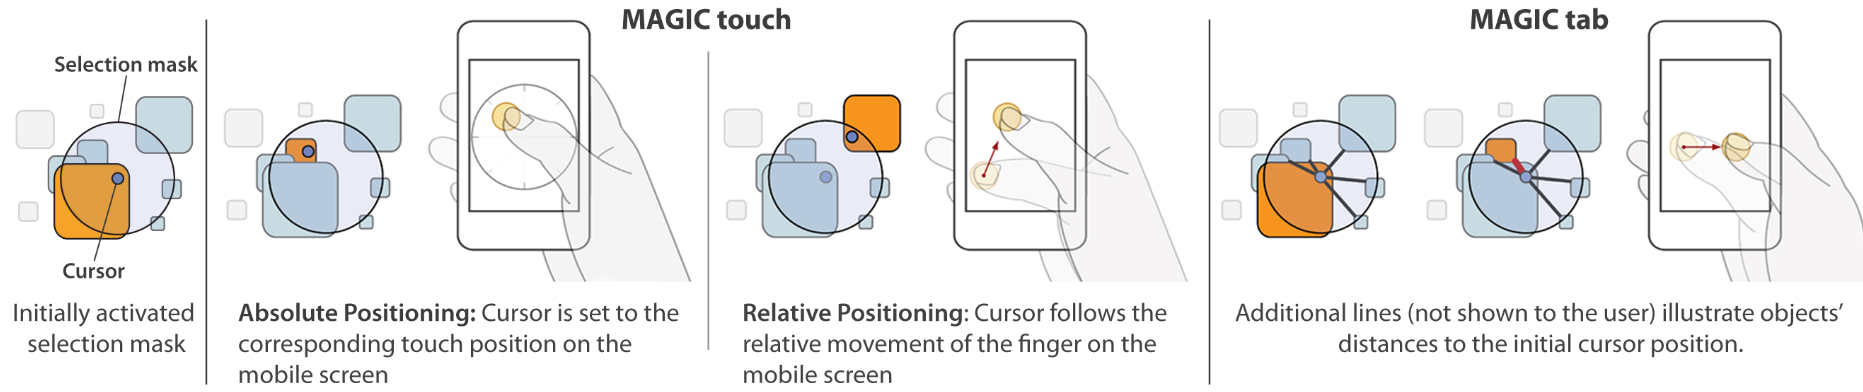
\includegraphics[width=\textwidth]{figures/ch2/lookandtouch}
		\caption[\emph{Look \&{} Touch -- principe}]{Fonctionnement des quatre premiers modes de sélection en cascade de la famille \emph{Look \&{} Touch}. Crédit : \cite{stellmach2012look}.}
		\label{fig:lookandtouch}
	\end{figure}
	
	\begin{figure}[!htb]
		\centering
		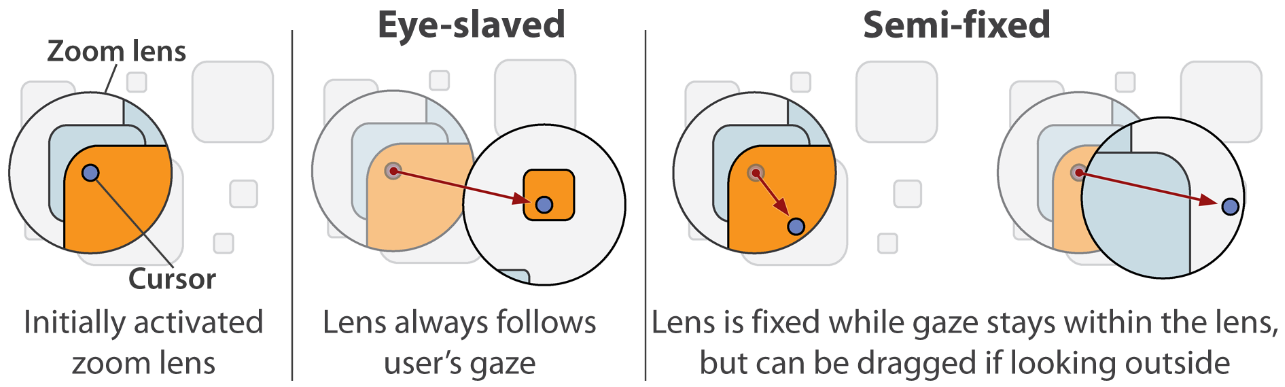
\includegraphics[width=0.8\textwidth]{figures/ch2/lookandtouch2}
		\caption[\emph{Look \&{} Touch -- principe II}]{Fonctionnement des deux derniers modes de sélection en cascade de la famille \emph{Look \&{} Touch}. Crédit : \cite{stellmach2012look}.}
		\label{fig:lookandtouch2}
	\end{figure}
	
	\paragraph{De bons résultats, sans vainqueur clair.}
	Stellmach \emph{et al.} ont évalué les variantes de \emph{Look \&{} Touch} sus-citées dans trois blocs de tâches : T1, avec des objets disjoints sur une grille 2D ; T2, avec une ligne d'objets 2D se chevauchant ; et T3, avec des objets 2D de tailles diverses se chevauchant.
	
	Diverses tailles et distances ont également été testées. Les temps de sélection et les taux d'erreurs ont été mesurés ; ils sont rapportés sur la figure~\ref{fig:latRes}. Si le \emph{Gaze-directed cursor} montre rapidement ses limites, les autres techniques fournissent de bonnes performances dans la plupart des cas, avec peut-être un léger avantage global à la technique \emph{MAGIC tab}. Du moins cette tendance est-elle confirmée par les impressions sujectives recueillies par Stellmach \emph{et al.}, et exposées sur la figure~\ref{fig:latSubj}.

	\begin{figure}[!htb]
		\centering
		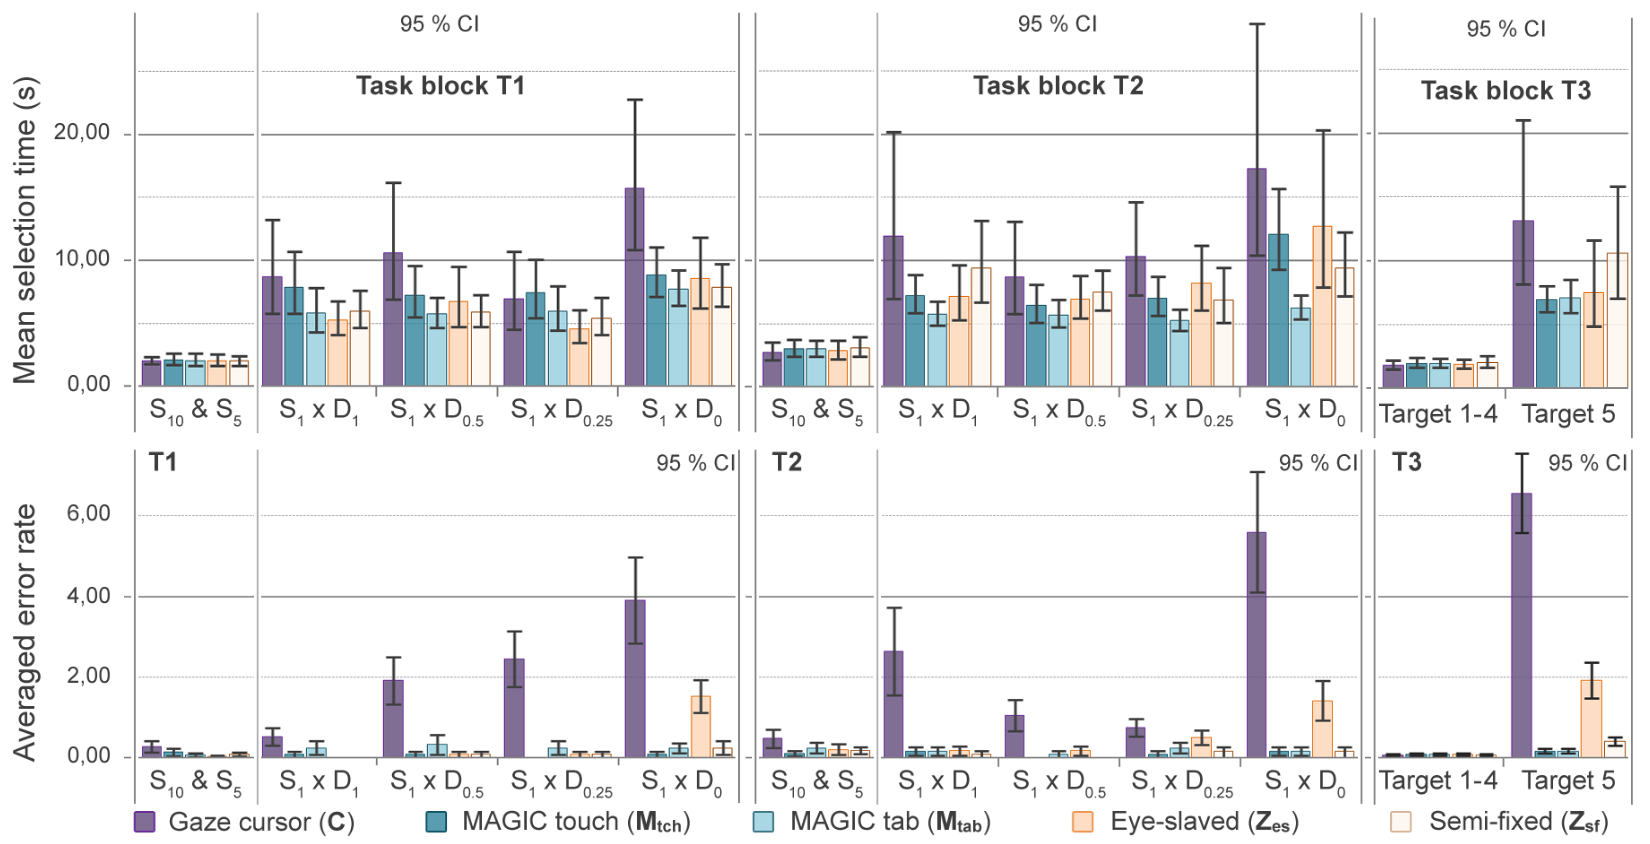
\includegraphics[width=\textwidth]{figures/ch2/latRes}
		\caption[\emph{Look \&{} Touch -- performances}]{Performances obtenues pour les diverses techniques de type \emph{Look \&{} Touch}. Les temps de sélection sont en haut, et les taux d'erreurs en bas. Les mentions $S_{i}$ et $D_{i}$ indiquent respectivement les différentes tailles et distances. Crédit : \cite{stellmach2012look}.}
		\label{fig:latRes}
	\end{figure}
	
	\begin{figure}[!htb]
		\centering
		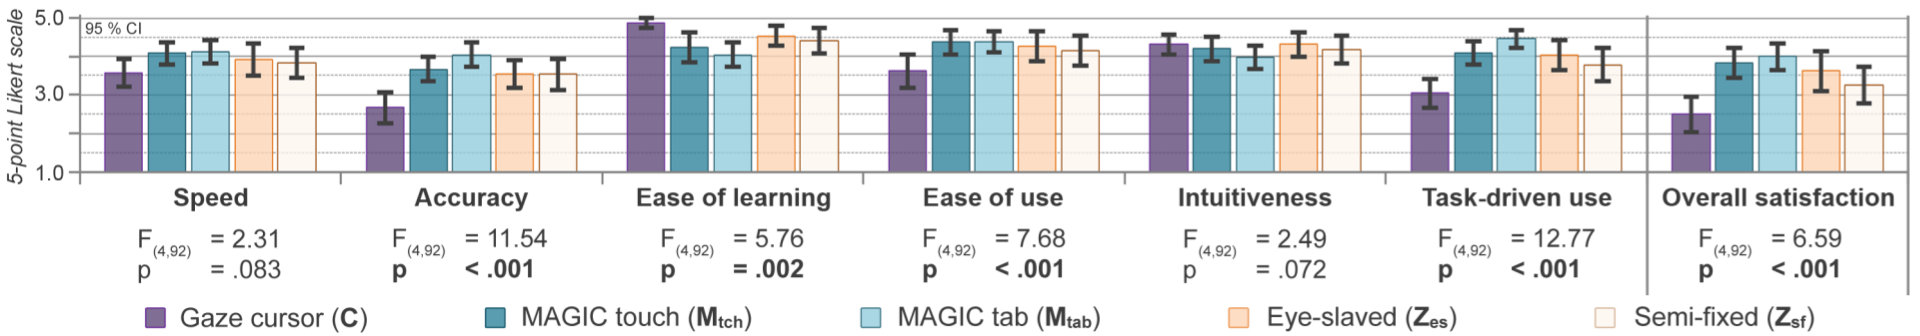
\includegraphics[width=\textwidth]{figures/ch2/latSubj}
		\caption[\emph{Look \&{} Touch -- impressions subjectives}]{Impressions subjectives recueillies par Stellmach \emph{et al.} auprès des sujets de l'évaluation des techniques \emph{Look \&{} Touch}. La technique \emph{MAGIC tab} l'emporte, mais d'une très courte tête. Crédit : \cite{stellmach2012look}.}
		\label{fig:latSubj}
	\end{figure}
	
	\paragraph{\emph{MAGIC tab} et le problème de linéarité.}
	Si, comme l'on vient de le voir, la technique \emph{MAGIC tab} sort légèrement du lot et se hisse en tête des résultats objectifs et subjectifs, elle souffre d'une limitation inhérente à sa nature : le temps de sélection dans la phase fine dépend de façon approximativement linéaire du nombre d'objets à parcourir, puisque l'utilisateur est contraint de faire ce parcours de façon linéaire.
	
	En comparaison, la plupart des processus de sélection sont accompagnés d'une relation logarithmique entre le nombre d'objets et le temps de sélection~\cite{hick1952rate, hyman1953stimulus}. L'on peut donc émettre des doutes sur la robustesse de \emph{MAGIC tab} dans des environnements très denses.
	
	Ajoutons que le comportement de cette technique avec des cibles mobiles pose question, puisque le menu contiendrait des objets n'étant plus nécessairement dans l'espace de pré-sélection au moment où l'utilisateur les parcourt. Cette perte de contexte spatial pourrait, dans le cas de cibles visuellement très proches (ou identiques) rendre la sélection impossible.
	
	\subsubsection{\emph{Sphere-casting refined by QUAD-menu
(SQUAD)}}
	Un exemple typique de méthode de sélection en cascade est la technique \emph{Sphere-casting refined by QUAD-menu
(SQUAD)}~\cite{kopper2011rapid}. Avec SQUAD, l'utilisateur commence par sélectionner un volume contenant sa cible ; puis, il affine progressivement sa sélection en choisissant le sous-ensemble de cibles contenant celle qu'il veut, via un menu à quatre options affichant tous les objets n'ayant pas encore été éliminés ; \emph{in fine}, le dernier objet restant est sélectionné. Aucune des sous-tâches de SQUAD ne nécessite d'être précis. Le fonctionnement de cette technique est illustré par la figure~\ref{fig:squad}.

	\begin{figure}[!htb]
		\centering
		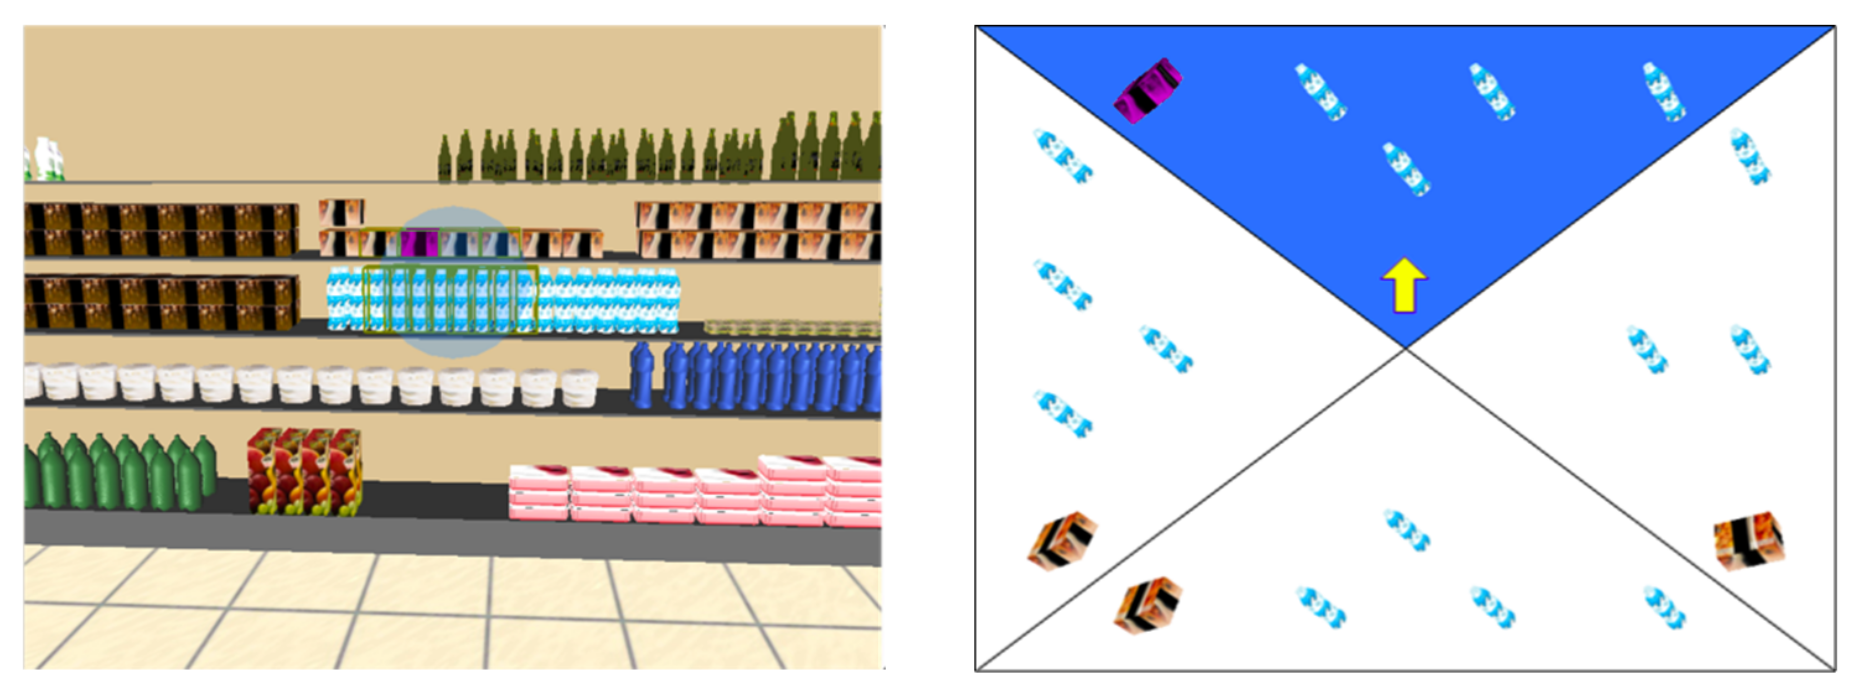
\includegraphics[width=\textwidth]{figures/ch2/squad}
		\caption[Fonctionnement de la technique SQUAD]{SQUAD : à gauche, la première étape de sélection, au cours de laquelle l'utilisateur pré-sélectionne une portion de l'espace à l'aide d'une sphère. À droite, la phase suivante, permettant d'affiner la sélection. Les objets pré-sélectionnés avec la sphère sont uniformément répartis dans quatre quadrants d'un menu, et l'utilisateur n'a plus qu'à choisir le quadrant contenant l'objet qu'il souhaite sélectionner. Les autres quadrants se vident, puis les objets du quadrant sélectionné sont répartis dans les quatre afin de permettre, dans une nouvelle étape, d'affiner encore la sélection. L'opération est répétée jusqu'à ce qu'il n'y ait plus qu'un objet, qui est sélectionné. Crédit : \cite{kopper2011rapid}.}
		\label{fig:squad}
	\end{figure}
	
	Bien que le procédé puisse paraître pénible, il permet d'affiner la sélection jusqu'au dernier élément en $log_{4}(n)$ étapes, où $n$ est le nombre d'objets pré-sélectionnés par la sphère au cours de la première étape. Naturellement, il faut ajouter à cela l'étape de pré-sélection. Au total, la sélection d'un objet parmi 256 se fait en seulement 5 étapes, où chaque étape peut être très rapide.
	
	En pratique, dans~\cite{kopper2011rapid}, SQUAD fut évaluée avec des objets uniformes : des sphères de rayons identiques. Seule la couleur variait, avec du gris pour des distracteurs et du rouge pour la cible à sélectionner, comme on le voit sur la figure~\ref{fig:squad2}. 
	
	\begin{figure}[!htb]
		\centering
		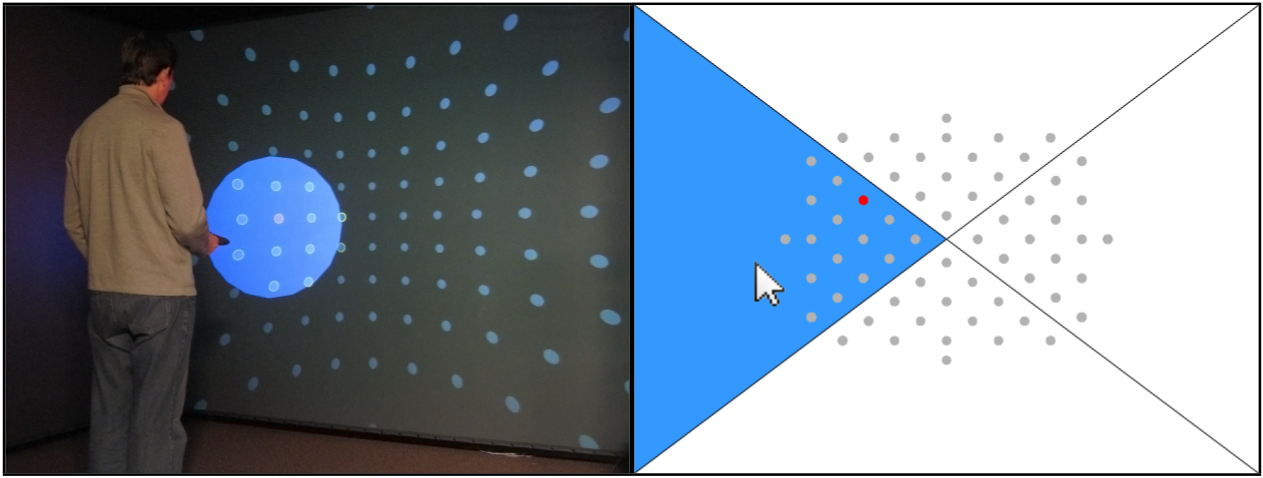
\includegraphics[width=\textwidth]{figures/ch2/squad2}
		\caption[La technique SQUAD -- évaluation]{SQUAD tel qu'évalué dans~\cite{kopper2011rapid}. Dans la première phase (à gauche) les petites sphères sont réparties sur la surface d'une grande sphère invisible centrée sur l'utilisateur, de sorte qu'elles sont toutes à la même distance de lui, afin qu'elles aient toutes une taille apparente égale une fois projetées sur l'écran. La cible à saisir est identifiée par sa couleur rouge. Seule l'orientation du périphérique de pointage était prise en compte dans la première phase, et les sujets avaient pour consigne de maintenir sa position dans une zone déterminée. Crédit : \cite{kopper2011rapid}.}
		\label{fig:squad2}
	\end{figure}
	
	\paragraph{Performances.}
	Les performances de SQUAD, comparée au \emph{raycasting} et en fonction du nombre de distracteurs sont détaillées sur la figure~\ref{fig:squadDensity}. On constate que SQUAD offre de meilleures performances en environnement dense, de moins bonnes en environnement peu dense, et des résultats comparables entre les deux. Les mêmes résultats sont présentés sur la figure~\ref{fig:squadSize}, mais en fonction de la taille des cibles. Comme attendu, les performances de SQUAD sont à peu près constantes tandis que le \emph{raycasting} est d'autant plus performant que les cibles sont grandes. De fait, la technique SQUAD est avantageuse avec de petites cibles, désavantageuses quand elles sont grandes, et à peu près équivalent entre les deux.
	
	\begin{figure}[!htb]
		\begin{subfigure}[t]{0.49\textwidth}
			\centering
			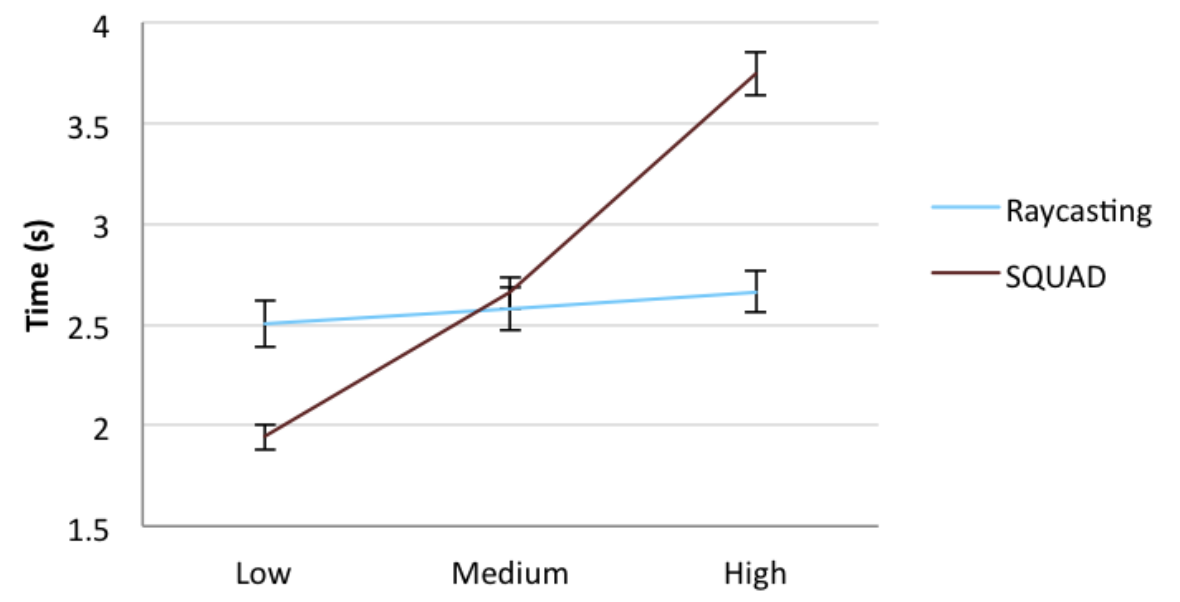
\includegraphics[width=\textwidth]{figures/ch2/squadDensity}
			\caption{Performances de SQUAD en fonction de la densité de distracteurs, comparées avec celle du \emph{raycasting}. Les performances de ce dernier ne sont pas significativement modifiées par la densité, même si une légère corrélation est visible, peut-être due à la recherche visuelle de la cible. Les performances de SQUAD sont fortement affectées, car le nombre d'étapes dépend de la densité. SQUAD brille dans les conditions de faible densité, mais se montre désavantageuse quand les distracteurs sont nombreux.}
			\label{fig:squadDensity}
		\end{subfigure}
		~
		\begin{subfigure}[t]{0.49\textwidth}
			\centering
			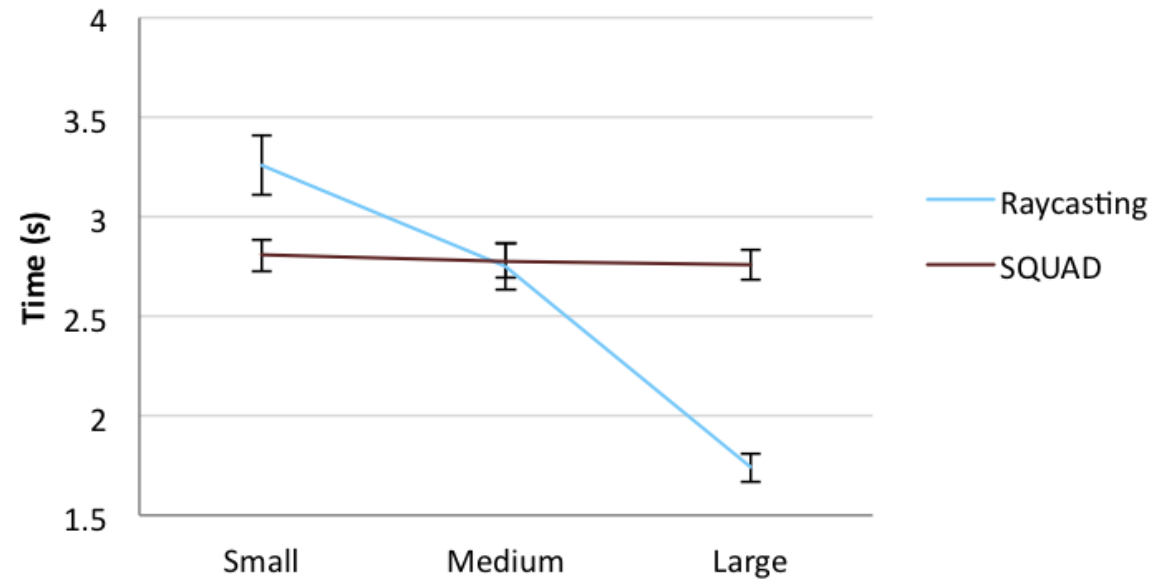
\includegraphics[width=\textwidth]{figures/ch2/squadSize}
			\caption{Performances de SQUAD comparées avec celles du \emph{raycasting}, en fonction de la taille des cibles, avec différentes densités de distracteurs. SQUAD est plus performante à faible densité, et capable de gérer de très petites cibles sans augmentation notable du temps de sélection, ce qui est intéressant pour certaines applications. Avec de grosses cibles, on préférera le \emph{raycasting}, en particulier dans ses formes améliorées.}
			\label{fig:squadSize}
		\end{subfigure}
		\caption[Performances de SQUAD]{Performances de SQUAD. Crédit : \cite{kopper2011rapid}.}
		\label{fig:squadPerf}
	\end{figure}
	
	Un récapitulatif de ces résultats est présenté sur la figure~\ref{fig:squadRecap}. On constate que la technique SQUAD gère très bien les petites cibles, mais voit ses performances chuter avec le nombre de distracteurs. Notons par ailleurs que le taux d'erreurs avec SQUAD était extrêmement faible, avec seulement 0,7~\%{}, ce qui est un atout notable pour cette technique. De fait, si l'on considérait non pas les temps de sélection, mais les temps de sélection normalisés par rapport aux erreurs, l'évaluation serait nettement plus favorable à SQUAD.
	
	\begin{figure}[!htb]
		\centering
		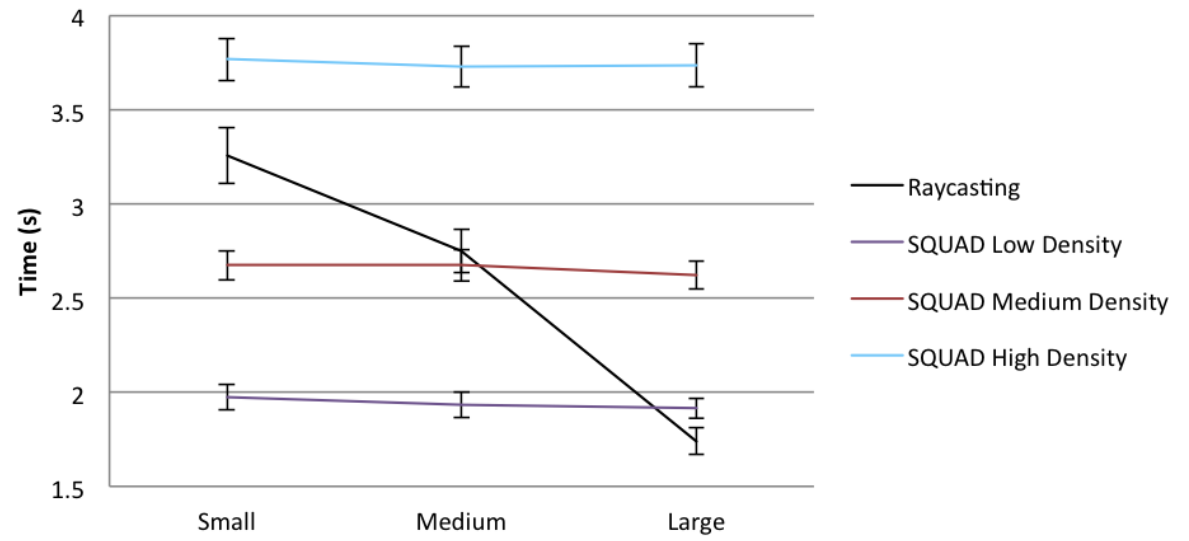
\includegraphics[width=0.65\textwidth]{figures/ch2/squadRecap}
		\caption[SQUAD -- résultats : taille]{Performances de SQUAD en fonction de la taille de la cible, comparées avec celles du \emph{raycasting}. Les performances de SQUAD ne sont pas significativement modifiées par la taille, même si une légère corrélation négative est visible, peut-être due à la recherche visuelle de la cible quand elle est petite. Les performances du \emph{raycasting} sont fortement affectées, puisqu'une petite cible a un ID bien plus élevé. SQUAD brille particulièrement avec de petites cibles, mais se montre désavantageuse quand elles sont grandes. Crédit : \cite{kopper2011rapid}.}
		\label{fig:squadRecap}
	\end{figure}
	
	\subsubsection{\emph{Disambiguation Canvas}}
	La technique du \emph{Disambiguation Canvas}~\cite{debarba2013disambiguation} est un autre exemple de technique de sélection en cascade, et est illustrée par la figure~\ref{fig:dCanvas}.
		 
	\begin{figure}[!htb]
		\centering
		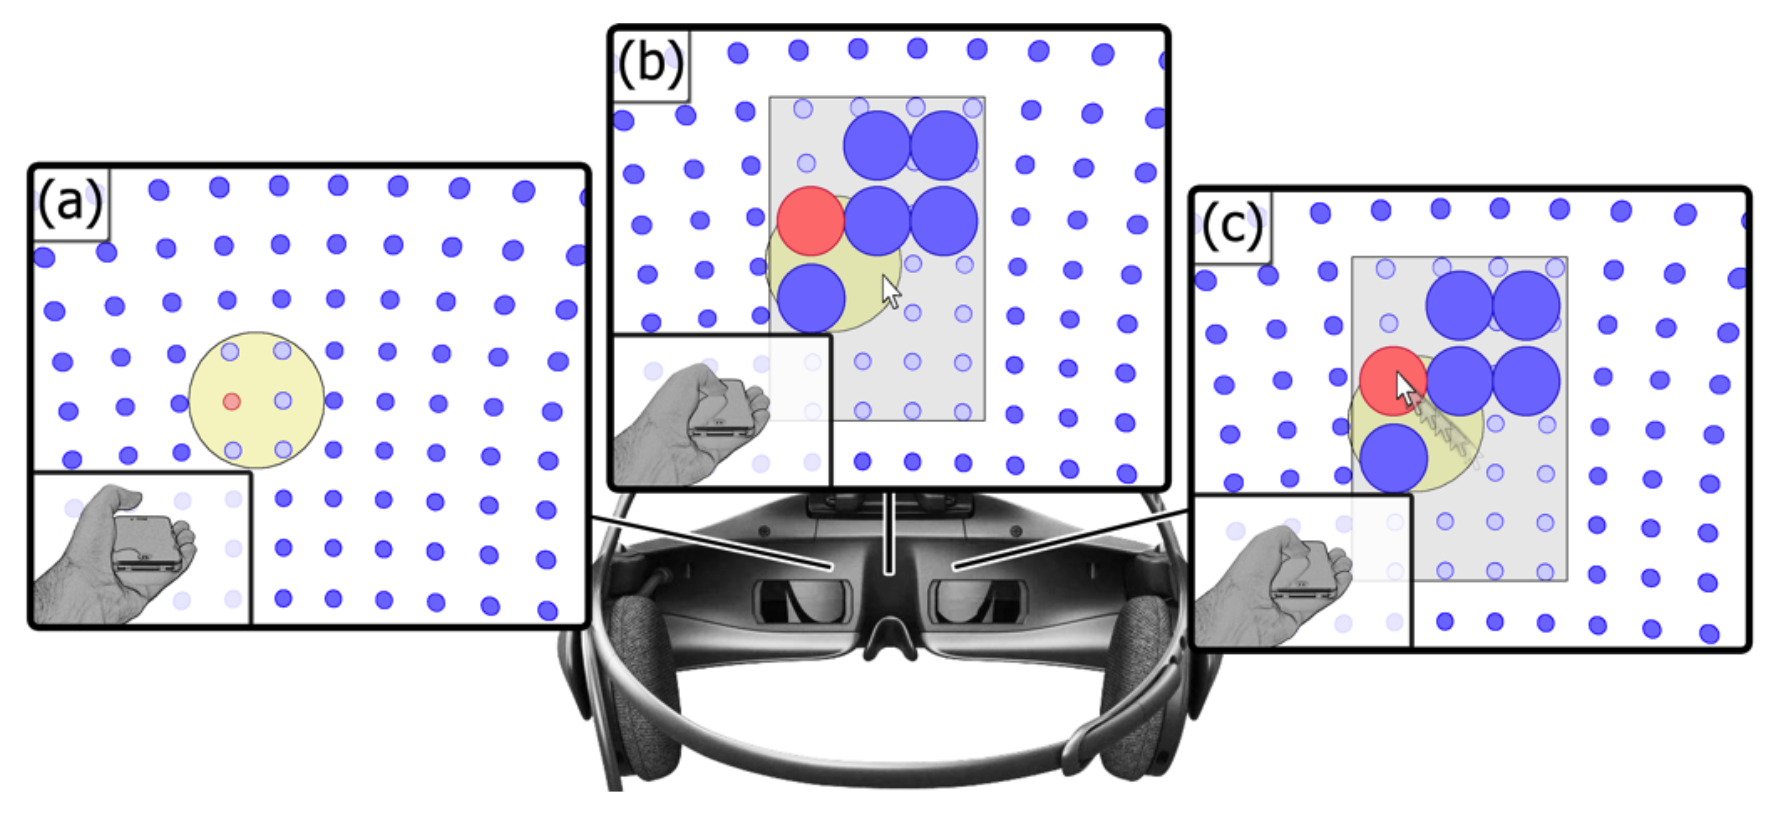
\includegraphics[width=\textwidth]{figures/ch2/dCanvas}
		\caption[\emph{Disambiguation Canvas}]{\emph{Disambiguation Canvas}. (a) : L'utilisateur pointe vers la région de l'espace où l'objet de son intérêt est situé ; cette pré-sélection se fait par \emph{volume casting}, c'est-à-dire que le périphérique de pointage contrôle un volume de sélection dans l'espace virtuel. (b) : Une fois la pré-sélection faite, une \og toile \fg{} (\emph{canvas}) de sélection (un rectangle semi-transparent) s'ouvre, les cibles pré-sélectionnées y sont disposées et agrandies. La toile de sélection correspond à un \emph{mapping} absolu de l'écran tactile d'un périphérique de saisie, ce qui permet à l'utilisateur de sélectionner la cible avec son pouce. Cette technique est compatible avec les HMD, et n'affiche pas le petit encadré en bas à gauche de chaque image, inséré ici à des fins illustratives. Crédit : \cite{debarba2013disambiguation}.}
		\label{fig:dCanvas}
	\end{figure}
	
	La figure~\ref{fig:dCanvas2} fournit une illustration supplémentaire et peut-être un peu plus claire de cette technique. Elle a pour avantage de ne nécessiter qu'un \emph{smartphone} comme périphérique de pointage pour la phase grossière, et de le réutiliser pour la sélection finale dans la phase fine. Dans la première, il est utilisé pour faire une pré-sélection à l'aide d'une sphère, comme dans SQUAD~\cite{kopper2011rapid} ; dans la seconde, les objets pré-sélectionnés sont arrangés dans un rectangle de même ratio d'aspect que l'écran du téléphone, et l'utilisateur n'a plus qu'à appuyer avec son pouce sur la zone de l'écran du téléphone correspondant à la zone du rectangle de sélection où se trouve la cible (se rapporter à la figure~\ref{fig:dCanvas} pour plus de clarté).
	
	\begin{figure}[!htb]
		\centering
		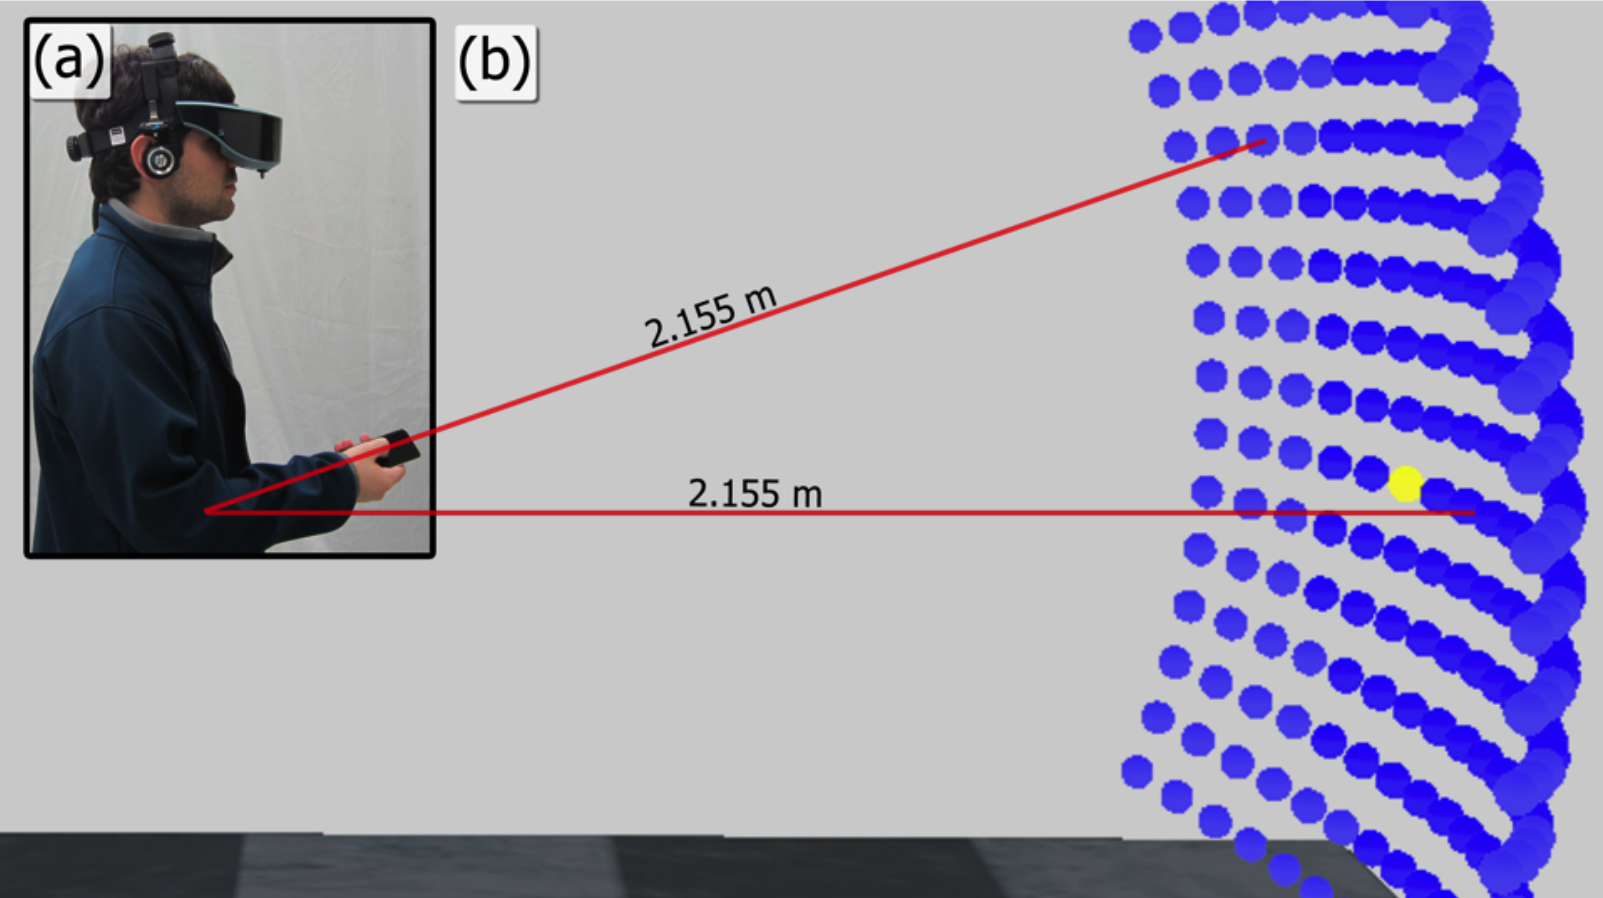
\includegraphics[width=0.80\textwidth]{figures/ch2/dCanvas2}
		\caption[\emph{Disambiguation Canvas}, bis]{Fonctionnement du \emph{Disambiguation Canvas}. En (a), une photo d'un utilisateur de la technique, équipé d'un HMD et d'un pointeur ; en (b), l'espace virtuel utilisé pour évaluer la technique. Comme dans l'évaluation originale de SQUAD, les petites sphères sont réparties sur la surface d'une grande sphère invisible~\cite{kopper2011rapid}, ce qui permet d'uniformiser leurs tailles apparentes. Crédit : \cite{debarba2013disambiguation}.}
		\label{fig:dCanvas2}
	\end{figure}
	
	Pour définir un agencement optimal des objets dans la deuxième phase, dite de désambiguïsation, Debarba \emph{et al.} ont opté pour une étape de calibrage présentée sur la figure~\ref{fig:dCanvasLayout}.
	
	\begin{figure}[!htb]
		\centering
		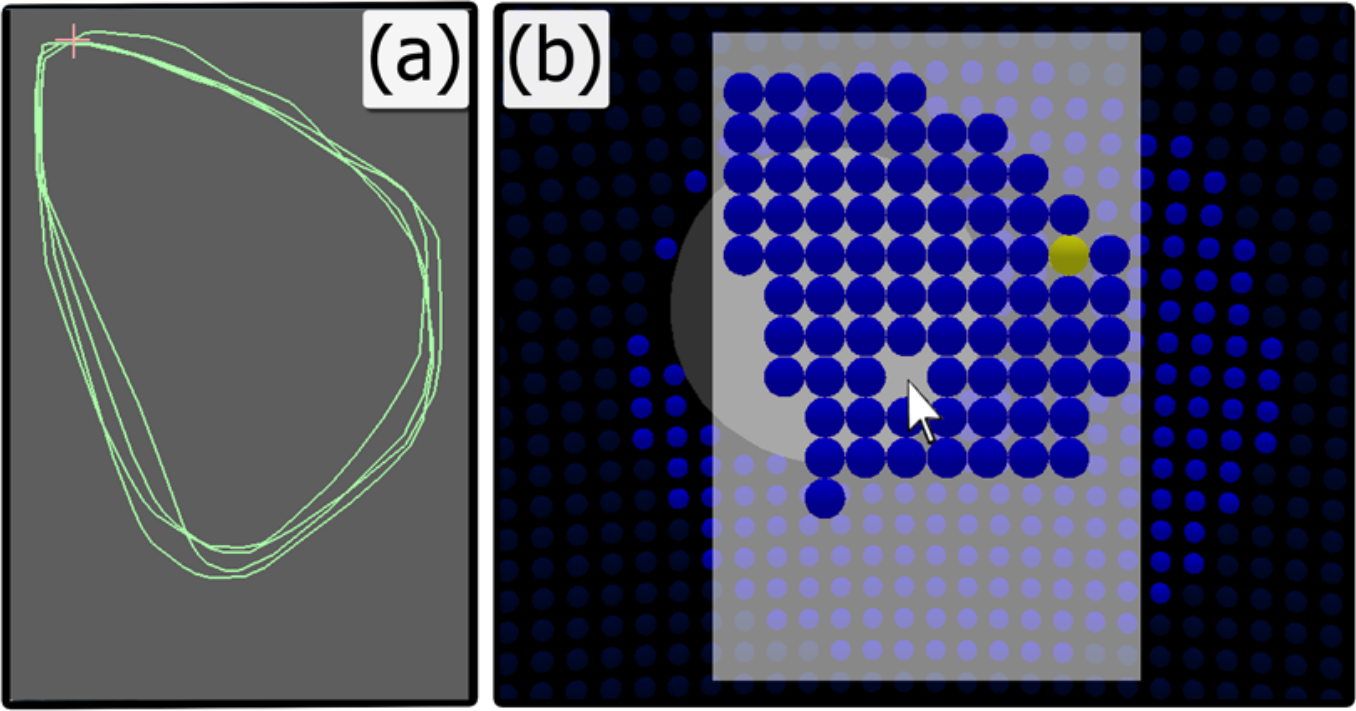
\includegraphics[width=0.8\textwidth]{figures/ch2/dCanvasLayout}
		\caption[\emph{Disambiguation Canvas} -- calibrage]{(a) : étape de calibrage pour la deuxième phase du \emph{Disambiguation Canvas}. On demande ici à l'utilisateur de faire le tour de l'écran avec son pouce, en essayant de s'approcher des bords. Il en résulte un motif fermé représentant l'espace que l'utilisateur peut atteindre confortablement. (b) : cet espace est utilisé pour répartir les objets, dont la cible, que l'utilisateur pourra ainsi sélectionner aisément. Par défaut, l'emplacement du le curseur est laissé vide, pour éviter les sélections accidentelles et faciliter l'annulation en cas d'erreur au cours de la première phase. Crédit : \cite{debarba2013disambiguation}.}
		\label{fig:dCanvasLayout}
	\end{figure}
	
	Notez que les objets pré-sélectionnés sont aggrandis ou rapetissés pour emplir l'espace de sélection dans la seconde phase. De fait, leur taille dans cette phase dépend essentiellement du nombre d'objets pré-sélectionnés dans la première, plus que de la taille des objets eux-mêmes. De fait, la difficulté effective de sélection des objets dépend plus du nombre d'objets pré-sélectionnés (donc indirectement de la densité de distracteurs) que de la taille réelle de l'objet visé, comme le montre la figure~\ref{fig:dCanvasDensity}.
	
	\begin{figure}[!htb]
		\centering
		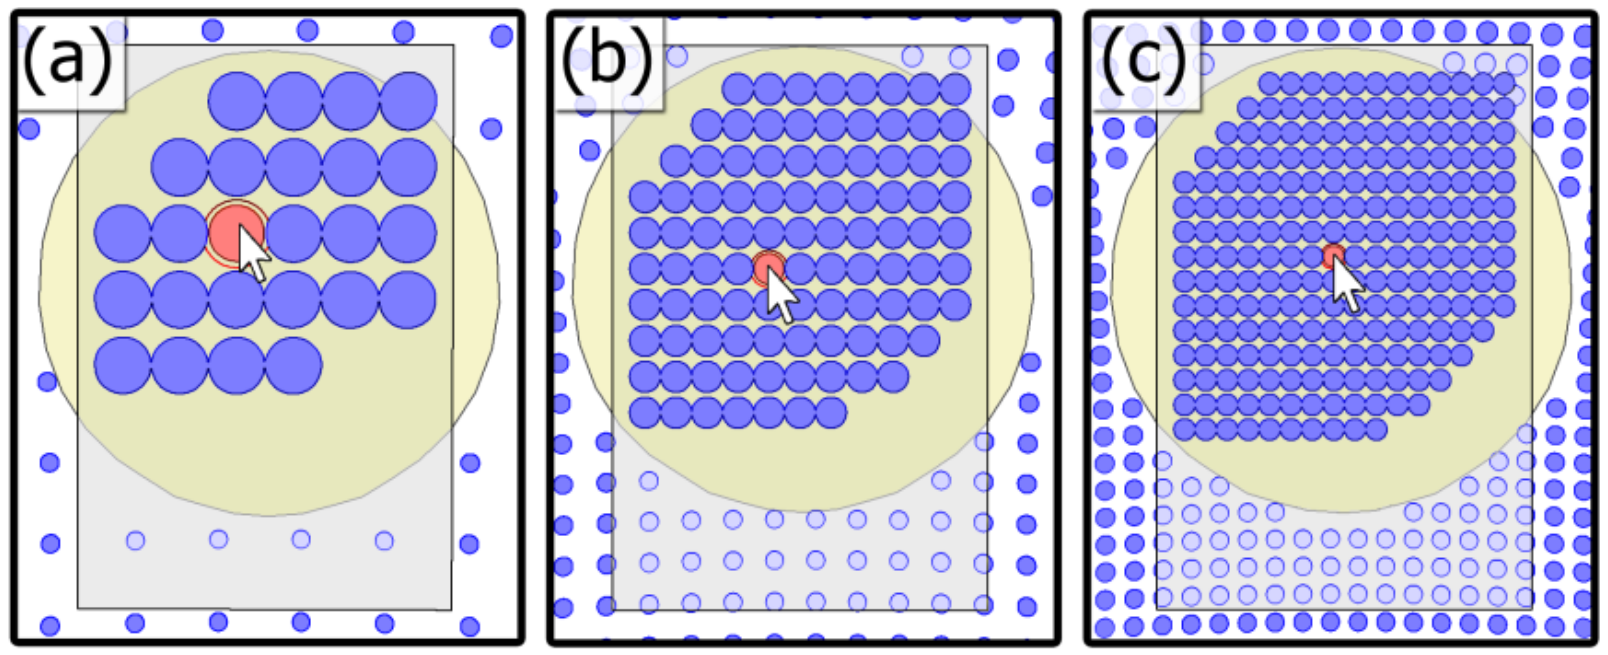
\includegraphics[width=0.80\textwidth]{figures/ch2/dCanvasDensity}
		\caption[\emph{Disambiguation Canvas} -- densité]{La difficulté de sélection avec le \emph{Disambiguation Canvas} dépend du nombre d'objets pré-sélectionnés dans la première étape. (a) : 25 objets peuvent être sélectionnés, et sont de fait assez gros ; (b) : ils sont 97, et de taille moyenne ; (c) : ils sont 224 et nettement plus petits. La loi de Fitts nous indique que les cibles seront plus difficiles à sélectionner en environnement dense, du fait de leur taille réduite. Crédit : \cite{debarba2013disambiguation}.}
		\label{fig:dCanvasDensity}
	\end{figure}
	
	\paragraph{Performances.}
	Les performances du \emph{Disambiguation Canvas} sont présentées sur la figure~\ref{fig:dCanvasRCPerf}, comparées à celle du \emph{raycasting} classique. Ainsi, l'on constate que cette technique ne fait mieux que le \emph{raycasting} qu'à condition que la densité soit faible ou que les cibles soient petites --- et \emph{a fortiori} les deux à la fois. Ce résultat n'est pas surprenant puisque la sélection en cascade implique nécessairement un coût en divisant la tâche en plusieurs parties, mais ce coût peut rester acceptable si la difficulté de la tâche est suffisamment élevée.
	
	On notera que les taux d'erreurs du \emph{Disambiguation Canvas} sont toujours inférieurs à ceux du \emph{raycasting}, et parfois de beaucoup. C'est une caractéristique courante de la sélection en cascade, qui implique intrinsèquement un biais en faveur de la précision dans le compromis vitesse/précision inhérent à toute tâche de pointage.
	
	\begin{figure}[!htb]
		\centering
		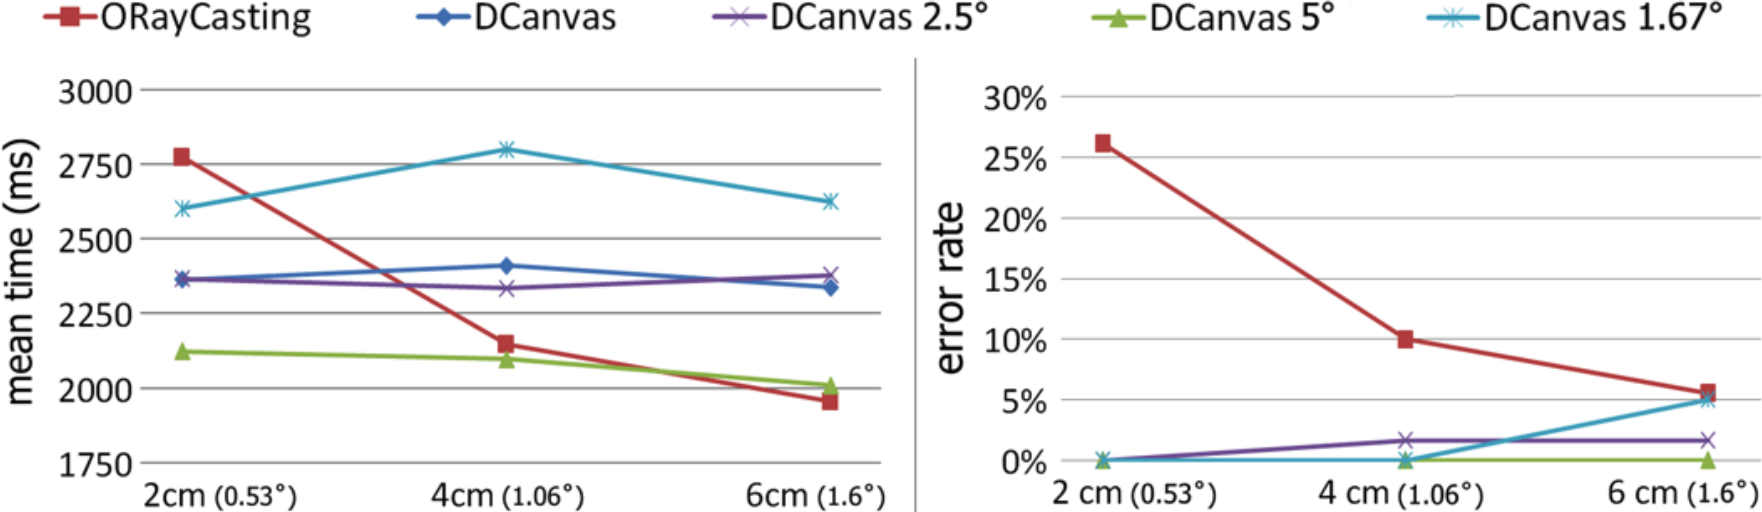
\includegraphics[width=\textwidth]{figures/ch2/dCanvasRCPerf}
		\caption[\emph{Disambiguation Canvas} -- performances I]{Performances du \emph{Disambiguation Canvas}, comparées à celles du \emph{raycasting}, en fonction de la taille des cibles. Pour le \emph{Disambiguation Canvas}, les résultats sont séparés en fonction de la distance angulaire entre les cibles, c'est-à-dire en fonction de leur densité. Plus cette densité est élevée (i.e. plus les angles sont faibles) plus la sélection est difficile car les cibles deviennent petites dans la phase de sélection fine. Les temps de sélection sont affichés sur le graphique de gauche, et les erreurs sur celui de droite. Crédit : \cite{debarba2013disambiguation}.}
		\label{fig:dCanvasRCPerf}
	\end{figure}

	Enfin, précisons que l'agencement calibré des objets décrit sur la figure~\ref{fig:dCanvasLayout} n'était pas utilisé dans cette étude, puisqu'il a été inspiré par les retours des utilisateurs au cours de celle-ci. De fait, on peut supposer avec cette optimisation, les résultats obtenus seraient légèrement meilleurs. Par ailleurs, les utilisateurs rapportent une préférence marquée pour le \emph{Disambiguation Canvas} par rapport au \emph{raycasting}, surtout pour les cibles difficiles, et de même une diminution de la fatigue ressentie.
	
	Pour comparer leur technique à SQUAD, Debarba \emph{et al.} ont légèrement modifié celle-ci en ajoutant après chaque étape \og d'affichage \fg{} une animation de 200 ms repositionnant les objets dans les quadrants vidés. Quoique cette animation ait un coût, elle permet à l'utilisateur de ne pas perdre la cible qu'il souhaite sélectionner, et donc d'éviter une nouvelle phase de recherche visuelle. Pour des contextes où les objets se ressemblent (voire sont identiques) c'est un compromis qui peut être avantageux (voire indispensable). De plus, l'utilisateur peut déplacer son rayon de sélection pendant l'animation.
	
	Les résultats du \emph{Disambiguation Canvas} comparé à SQUAD sont présentés sur la figure~\ref{fig:dCanvasSPerf}, et sont en faveur de ce premier, sans appel. Plus les objets sont nombreux, plus son avantage croît. On peut toutefois s'interroger sur la solidité de ce résultat avec des objets extrêmement nombreux, puisque la convergence logarithmique de SQUAD permet en principe de gérer un nombre d'objets colossal sans dégradation catastrophique des performances, tandis que le \emph{Disambiguation Canvas} pourrait voir ses performances s'effrondrer lorsque les cibles deviennent trop petites pour être sélectionnées avec une pression du pouce.	
	
	\begin{figure}[!htb]
		\centering
		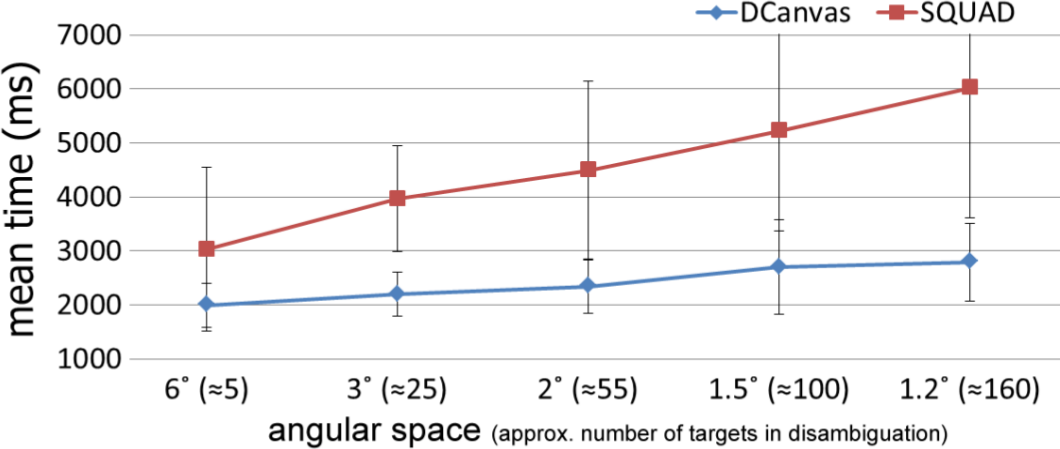
\includegraphics[width=0.85\textwidth]{figures/ch2/dCanvasSPerf}
		\caption[\emph{Disambiguation Canvas} -- performances II]{Temps de sélection du \emph{Disambiguation Canvas}, comparées à celles de SQUAD, en fonction du nombre de cibles. Les résultats sont clairement en faveur de la première technique sur l'intervalle testé. Crédit : \cite{debarba2013disambiguation}.}
		\label{fig:dCanvasSPerf}
	\end{figure}
	
	Au-delà des temps de sélection, les taux d'erreurs deviendraient certainement problématiques dans ce cas-là, alors qu'ils devraient rester à peu près stables pour SQUAD. Sur l'intervalle de tailles testé, SQUAD a d'ailleurs un léger avantage sur ce plan, avec 0,9~\%{} d'erreurs contre 1,8~\%{} pour le \emph{Disambiguation Canvas}, mais ce dernier résultat reste très bon. Les impressions subjectives des utilisateurs sont grossièrement similaires pour les deux techniques.
		 
	\subsubsection{Le problème de la perte du contexte}
	Les techniques de sélection en cascade pouvant prendre des formes diverses, leurs avantages et inconvénients sont également divers. Néanmoins, elles ont pour principe commun de travailler successivement à différentes échelles, ce qui peut être perturbant en environnement immersif, particulièrement lorsque l'on cherche à maintenir une correspondance entre l'espace moteur et l'espace virtuel. Néanmoins, si les gains de performances offerts par la sélection en cascade sont importants, cette perturbation pourrait être une contrepartie acceptable.
	
	Les choix faits dans la conception du \emph{Disambiguation Canvas} sont différents de ceux de SQUAD, et les évaluations de ces techniques le montrent. Toutefois, les inconvénients majeurs de ces deux techniques sont sensiblement les mêmes, à savoir une perte de contexte en passant d'une phase à l'autre, et de grandes difficultés à reconnaître l'objet à sélectionner s'il est visuellement proche des distracteurs, ou \emph{a fortiori} identique.
	
	Pour pallier ce problème, Debarba \emph{et al.} proposent de gérer la transition entre les deux phases avec une animation permettant de déplacer les objets de l'espace virtuel 3D d'origine vers le rectangle de sélection finale de façon \og douce \fg{} et progressive, afin que l'utilisateur ne perde pas sa cible des yeux et puisse la retrouver aisément. Dans une certaine mesure, le contexte spatial (local) est préservé, mais il est significativement déformé en règle générale. Cette solution, que les auteurs ont mise en \oe{}uvre mais pas encore évaluée, est illustrée par la figure~\ref{fig:dCanvasContext}.
	
	\begin{figure}[!htb]
		\centering
		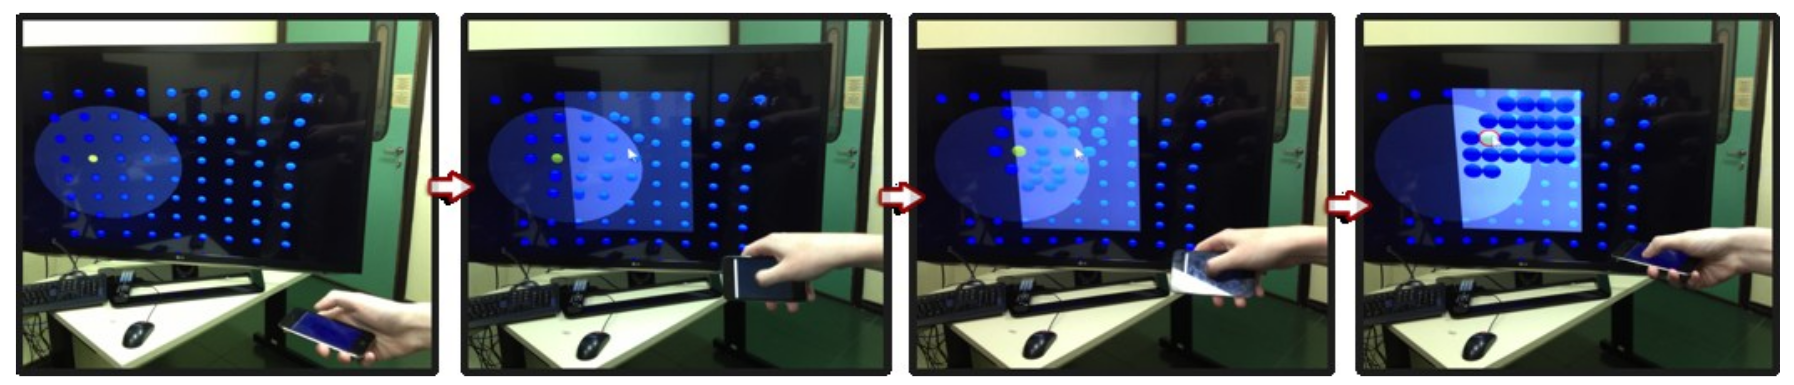
\includegraphics[width=\textwidth]{figures/ch2/dCanvasContext}
		\caption[\emph{Disambiguation Canvas} -- animation de transition]{Animation pendant la transition entre la phase de pré-sélection du \emph{Disambiguation Canvas} et la phase de disambiguïsation. Les objets sont réarrangés \og en douceur \fg{} ce qui permet à l'utilisateur de suivre la cible des yeux afin de ne pas la perdre, et de préserver, dans une certaine mesure, le contexte spatial. Crédit : \cite{debarba2013disambiguation}.}
		\label{fig:dCanvasContext}
	\end{figure}
	
	Bien que ce palliatif puisse améliorer les performances de sélection quand les objets se ressemblent, on peut douter de son efficacité quand ils sont identiques. De plus, le contexte spatial demeure très dégradé en passant d'une phase à l'autre, et les cibles ne sont, là encore, que statiques. Il apparaît donc difficile d'appliquer le \emph{Disambiguation Canvas} à des contextes caractérisés par des objets semblables, nombreux et mobiles, tout comme SQUAD.
	
	Cela ne revient pas à rejeter le principe de la sélection en cascade pour les applications qui nous intéressent, mais à souligner que les solutions existantes sont généralement peu adaptées à de telles tâches, et qu'une technique de sélection en cascade appropriée nécessiterait probablement d'être pensée pour les cibles mobiles dès le départ.
	
	\subsection{Techniques fondées sur l'augmentation des objets}
	Certaines techniques se fondent sur la loi de Fitts et son énoncé de l'importance de la largeur de la cible pour faciliter la sélection en augmentant les cibles, de façon à les agrandir. Attardons-nous sur deux d'entre elles.
	
	\subsubsection{\emph{(Bubble) Comet}}
	Avec \emph{Comet}~\cite{hasan2011comet}, chaque cible potentielle laisse derrière elle une traînée (ou queue) qui peut être sélectionnée à la place de la cible elle-même, comme le montre la figure~\ref{fig:comet}.

	\begin{wrapfigure}{O}{0.5\textwidth} % Capital O makes the figure float, because that's totally intuitive and obvious.
		\centering
		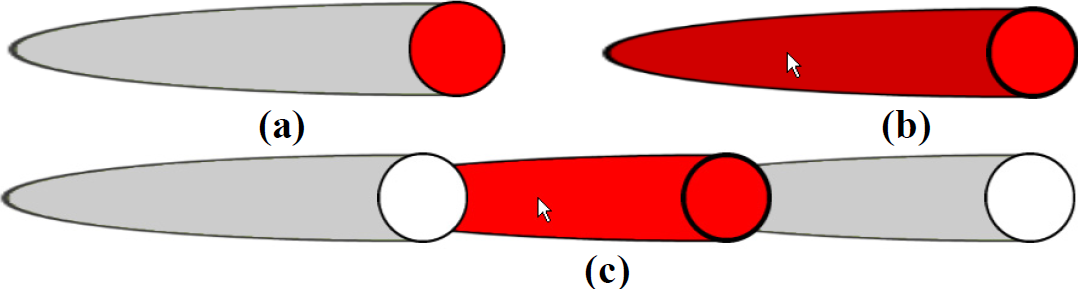
\includegraphics[width=0.46\textwidth]{figures/ch2/comet}
		\caption[La technique \emph{Comet}]{(a) La cible et sa queue de comète. (b) La queue est mise en surbrillance lorsque le curseur passe dessus. (c) Les queues peuvent être recouvertes par les cibles ajdacentes. Crédit : \cite{hasan2011comet}.}
		\label{fig:comet}
	\end{wrapfigure}
	
	Cela revient à augmenter la taille effective des cibles. Attendu que cela s'applique aux cibles et pas aux curseurs, \emph{Comet} peut être combinée à une technique de curseur, par exemple le \emph{Bubble Cursor} ou \emph{DynaSpot}. Hasan \emph{et al.} ont montré que cette technique permet de significativement améliorer les temps de sélection et les taux d'erreurs pour les cibles mobiles en 2D~\cite{hasan2011comet}, comme le montrent les résultats compilés sur les figures~\ref{fig:cometGhostTimes}, \ref{fig:cometGhostErrors} et~\ref{fig:cometGhostPredictability}.

	\subsubsection{\emph{AttachedShock}}
	\emph{AttachedShock}~\cite{you2012attachedshock, you2014attachedshock}. est une technique développée pour répondre à un besoin plutôt spécifique à la réalité augmentée : la sélection d'objets \og fuyants \fg{} : lorsqu'un utilisateur se déplace dans une direction (à pied ou dans un véhicule) les objets à côté desquels il passent quittent son champ de vision rapidement, et de plus en plus vite à mesure que qu'ils s'approchent des bords du champ de vision, comme l'illustre la figure~\ref{fig:as2dspeed}.

	\begin{SCfigure}
		%\centering
		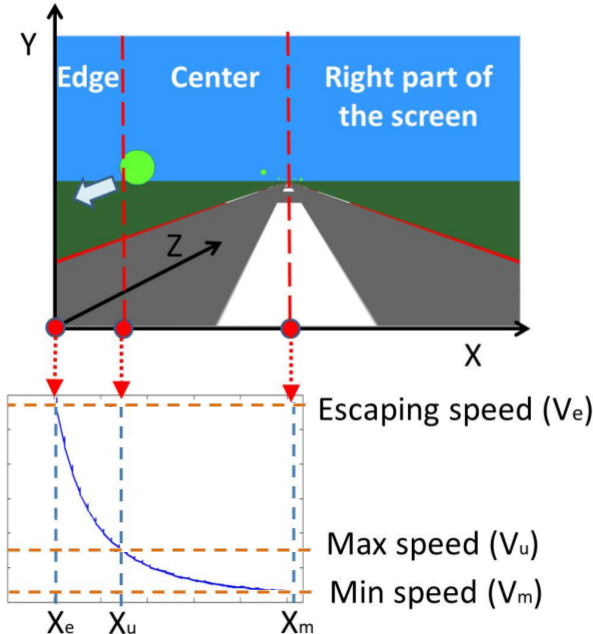
\includegraphics[scale=0.35]{figures/ch2/as2dspeed}
		\caption[\emph{AttachedShock}, profil de vitesse]{Vue d'un utilisateur dans une voiture, fixant la route. Des objets (les sphères vertes) attirent son attention. Ils sont fixés au sol, mais leur vitesse relative (par rapport au référentiel de la voiture) est celle de la voiture dans le référentiel terrestre. Une fois projetée sur un écran 2D, elle varie considérablement en fonction de la distance de l'objet au centre de l'écran. On peut parler de \emph{vitesse apparente}. Crédit : \cite{you2012attachedshock}.}
		\label{fig:as2dspeed}	
	\end{SCfigure}
	
	Pour faciliter la sélection de telles cibles sans trop augmenter l'encombrement visuel (\emph{clutter}) de la scène, les auteurs d'\emph{AttachedShock} ont choisi d'ajouter aux objets apparemment en mouvement une onde de choc, comme sur la figure~\ref{fig:asas}. Cette onde est augmente l'objet en facilite la sélection. \emph{AttachedShock} fait donc partie de la famille des techniques de sélection qui cherchent à faciliter la sélection en augmentant la taille effective des cibles. La sélection se fait en effet en \og traversant \fg{} l'onde de choc d'un objet, ce qui permet aux utilisateurs d'effectuer un mouvement balistique sans avoir à ralentir comme ils le devraient avec une cible non augmentée.
	
	\begin{figure}[!htb]
		\centering
		\includegraphics[width=0.70\textwidth]{figures/ch2/asas}
		\caption[\emph{AttachedShock}, onde de choc]{À gauche, une représentation schématique de la réelle onde de choc d'un avion supersonique (un \emph{Concorde}). À droite, une cible mobile (la sphère verte) accompagnée de son onde de choc telle qu'elle est représentée par \emph{AttachedShock}. Cette onde vient augmenter la représentation visuelle de la cible afin d'en faciliter la sélection. Crédit : ~\cite{you2012attachedshock}.}
		\label{fig:asas}
	\end{figure}
	
	Cette technique a pour particularité de le faire en limitant l'encombrement visuel et en optant pour une augmentation visuelle pouvant être perçue comme \og naturelle \fg{} --- plus par habitude des ondes de choc qui se propagent dans l'eau que de celles générées par les avions supersoniques, sans doute. Les auteurs ont comparé \emph{AttachedShock} à d'autres techniques de référence, dont bien sûr un simple curseur ponctuel mais aussi un curseur zonal, ainsi que la technique \emph{Comet}, présentée plus haut.

	La technique \emph{AttachedShock} s'est montrée meilleure que toutes les autres dans cette évaluation, quoique de peu pour le temps de sélection. Les résultats détaillés sont illustrés par la figure~\ref{fig:asRes}. Dans les conditions du protocole de test mis en place par les auteurs, \emph{AttachedShock} permet une sélection rapide et fiable par rapport aux techniques existantes, avec un encombrement visuel très contenu.

	\begin{wrapfigure}{O}{0.5\textwidth} % Capital O makes the figure float, because that's totally intuitive and obvious.
		\centering
		\includegraphics[width=0.46\textwidth]{figures/ch2/asRes}
		\caption[\emph{AttachedShock}, performance]{Évaluation d'\emph{AttachedShock}. Le taux d'erreurs est en abscisse, le temps de sélection en ordonnée. \emph{AttachedShock} ne fait pas bien mieux qu'un curseur zonal en temps de sélection, mais s'illustre pas un taux d'erreurs très bas, et par un temps de sélection moyen qui demeure le meilleur, quoique de peu. Résultats tirés de~\cite{you2012attachedshock}.}
		\label{fig:asRes}
	\end{wrapfigure}
	
	\emph{AttachedShock} n'est toutefois pas sans limite. En effet, la densité de cibles testée par les auteurs est très faible, comme le montre la figure~\ref{fig:asDensity}. La technique n'ayant pas été évaluée avec une grande densité de cibles, il est impossible d'affirmer qu'elle fonctionnerait bien dans de telles conditions, mais l'on peut en douter compte tenu du fait qu'elle repose sur la possibilité qu'a l'utilisateur de se \og contenter \fg{} de mouvements balistiques sans mouvements correctifs, ce qui serait bien difficile avec les nombreux obstacles que de nombreux distracteurs constitueraient.
	
	\begin{figure}[!htb]
		\centering
		\includegraphics[width=0.9\textwidth]{figures/ch2/asDensity}
		\caption[\emph{AttachedShock}, densité de cibles]{Captures d'écran du dispositif d'évaluation d'\emph{AttachedShock}. À gauche, l'expérience est menée sur un segment de route rectiligne ; à droite, sur un segment courbe. La sphère rouge est la cible à sélectionner, tandis que les vertes sont des distracteurs. On constate que les distracteurs sont peu nombreux et qu'il est relativement peu probable de \og traverser \fg{} leur onde de choc en essayant d'atteindre cette de la cible. Crédit: \cite{you2012attachedshock}.}
		\label{fig:asDensity}
	\end{figure}
	
	En outre, dans cette évaluation les cibles sont fixées au sol, et donc ne se déplacent à l'écran qu'à l'horizontale. De fait, leurs ondes de choc se présentent toujours dans la même orientation. Or, dans bien des cas, les cibles peuvent changer de direction en cours de route, ce qui soumettrait logiquement ces ondes de choc à de fréquentes rotations. Dans ces condtions, déclencher un mouvement balistique pour traverser l'onde de choc sans mouvements correctifs serait sans doute beaucoup plus difficile.	Ainsi, si \emph{AttachedShock} présente un intérêt certain pour la sélection de cibles mobiles peu nombreuses (avec peu de distracteurs) se déplaçant à l'horizontale, son efficacité en environnement dense et/ou avec des cibles changeant souvent de direction, \emph{a fortiori} de manière imprévisible, demeure à démontrer. Et compte tenu du fonctionnement de la technique, on peut même s'attendre à une chute significative de son efficacité relative dans ces conditions.

	\subsubsection{Augmentation et\ldots{} encombrement visuel}
	Les techniques fondées sur l'augmentation ont un inconvénient commun : l'encombrement visuel significativement accru, et les deux techniques évaluées ici ne font pas exception. De plus, elles modifient la représentation visuelle des cibles, et en particulier de leur forme. Pour certaines applications, par exemple les simulations moléculaires (dans lequelles la perception des formes des molécules est absolument critique) ce point est particulièrement gênant. Naturellement, le haut niveau d'encombrement visuel est d'autant plus problématique que l'environnement de départ est dense et présente un haut degré d'occultation.
	
	\subsection{Techniques de prédiction de la trajectoire du curseur}
	Une classe de techniques consiste à analyser une partie du mouvement du curseur de sélection pour tenter d'estimer son point d'arrivée, donc la cible visée par l'utilisateur, et ainsi accélérer la sélection. Nous allons ici en analyser quelques-unes.
	
	\subsubsection{Le \emph{Delphian Desktop}}
	Le \emph{Delphian Desktop}~\cite{asano2005predictive} est une technique de prédiction de la trajectoire du curseur, qui analyse sa position dans le temps pour essayer de déterminer si un pic de vélocité pour le mouvement en cours a été atteint. Il s'inspire d'observations sur les systèmes perceptif et moteur de l'humain, issues de diverses études de psychologie et kinésiologie~\cite{accot2003refining, graham1995pointing, graham1996physical, mackenzie1992extending, mackenzie1994prediction, takagi2002fundamental, walker1993spatial}.
	
	On sait en effet depuis une étude de Walker \emph{et al.}~\cite{walker1993spatial} que la hauteur du pic de vitesse d'un curseur croît avec la distance entre la cible et lui-même, avec un profil typique illustré par la figure~\ref{fig:delphianPeak}.

	\begin{figure}[!htb]
		\begin{subfigure}[t]{0.44\textwidth}
			\centering
			\includegraphics[width=\textwidth]{figures/ch2/delphianPeak}
			\caption{Vitesse du curseur. Il accélère au cours de la première phase (\emph{Plan time}) puis décélère (\emph{Adjustment time}).}
			\label{fig:delphianPeak}
		\end{subfigure}
		~
		\begin{subfigure}[t]{0.54\textwidth}
			\centering
			\includegraphics[width=\textwidth]{figures/ch2/delphianSpeedDist}
			\caption{Pic de vitesse du curseur en fonction de la distance à parcourir.}
			\label{fig:delphianSpeedDist}
		\end{subfigure}
		\caption[\emph{Delphian Desktop} : vitesse du curseur]{\emph{Delphian Desktop} : vitesse du curseur. Crédit : \cite{asano2005predictive}.}
		\label{fig:delphianCursor}
	\end{figure}
	
	Cette croissance est quant à elle illustrée par la figure~\ref{fig:delphianSpeedDist}.
	
	Le fonctionnement du \emph{Delphian Desktop} est basé sur les hypothèses suivantes :
	
	\begin{enumerate}
		\item Le curseur suit une ligne approximativement droite vers la cible ;
		\item La relation entre la distance à parcourir et le pic de vitesse du curseur est linéaire : $D = aPV + b$ où $D$ est la distance, $PV$ est le pic de vitesse, $a$ et $b$ sont des constantes.
	\end{enumerate}
	
	Ainsi, à partir du moment où l'on détermine que $PV$ a été atteint, si les constantes $a$ et $b$ sont correctement calibrées, il est possible de calculer D, et puisque le mouvement du curseur est supposé rectiligne, l'on peut estimer le point de destination du curseur. Ces constantes peuvent se calibrer par régression linéaire à partir d'enregistrement de trajectoires de curseur pour un individu donné --- en effet, pour des résultats optimaux, on calibrera les constantes différemment pour chaque personne.
	
	Dès lors que le \emph{Delphian Desktop} détermine que $PV$ est atteint, il déplace le curseur directement vers la position estimée. L'utilisateur n'a plus alors qu'à sélectionner la cible s'il est déjà dessus, ou effectuer le déplacement nécessaire (en principe petit) avant de le faire. Il est toutefois possible de modifier ce système afin que le curseur se déplace directement et automatiquement vers la cible la plus proche de la position finale estimée.
	
	\paragraph{Temps de sélection.}
	Les résultats obtenus par Asano \emph{et al.}~\cite{asano2005predictive} sont présentés sur la figure~\ref{fig:delphianTimes}. On y constate que le \emph{Delphian Desktop} est plus lent que la sélection non assistée lorsque les cibles sont proches, mais plus rapides quand elles sont distantes.
	
	\begin{figure}[!htb]
		\begin{subfigure}[t]{0.49\textwidth}
			\centering
			\includegraphics[width=\textwidth]{figures/ch2/delphianTimes}
			\caption{Temps de sélection en fonction de la distance entre le curseur et la cible, avec le \emph{Delphian Desktop} (\emph{Prediction}, en gris) et sans (\emph{Non-Prediction}, en blanc). Cette technique se montre contre-productive pour les faibles distances, mais bénéfiques quand les distances sont grandes.}
			\label{fig:delphianTimes}
		\end{subfigure}
		~
		\begin{subfigure}[t]{0.49\textwidth}
			\centering
			\includegraphics[width=\textwidth]{figures/ch2/delphianTimesErrors}
			\caption{Temps de sélection en fonction de l'erreur de prédiction de la direction du mouvement. Quelle que soit la distance considérée, le temps de mouvement croît fortement avec l'erreur de prédiction, car une grande erreur nécessite un plus grand mouvement correctif.}
			\label{fig:delphianTimesErrors}
		\end{subfigure}
		\caption[\emph{Delphian Desktop} -- performances]{\emph{Delphian Desktop} -- performances. Crédit : \cite{asano2005predictive}.}
		\label{fig:delphianPerf}
	\end{figure}

	Cette tendance est d'ailleurs mieux illustrée par la figure~\ref{fig:delphianTimesID}, qui met en évidence les différences de pentes entre les droites qui représentent le temps de sélection en fonction de l'indice de difficulté (ID) pour la sélection non assistée et pour le \emph{Delphian Desktop}. On peut supposer que, pour des cibles d'ID très élevé, celui-ci serait d'autant plus avantageux.
	
	Il convient néanmoins de remarquer que dasns l'étude d'Asano \emph{et al.}, seule la distance variait, pas la taille des cibles ; de fait, cette courbe de temps en fonction de l'ID pourrait ne pas tenir lorsque les variations d'ID proviennent de variations dans les tailles des cibles. C'est un point qui mérite d'être examiné.

	\begin{wrapfigure}{O}{0.5\textwidth} % Capital O makes the figure float, because that's totally intuitive and obvious.
		\centering
		\includegraphics[width=0.46\textwidth]{figures/ch2/delphianTimesID}
		\caption[\emph{Delphian Desktop} -- temps de sélection en fonction de l'ID]{Temps de sélection en fonction de l'ID, avec le \emph{Delphian Desktop} (\emph{Prediction}) et sans (\emph{Non-Prediction}). Cette technique est contre-productive pour les petites distances, mais bénéfique pour les grandes. La droite qui estime son temps de sélection en fonction de l'ID est d'une pente plus douce, ce qui est de bon augure pour d'hypothétiques cibles plus distantes. Crédit : \cite{asano2005predictive}.}
		\label{fig:delphianTimesID}
	\end{wrapfigure}
	
	Asano \emph{et al.} ont par ailleurs mesuré les erreurs de prédiction de la direction du mouvement, c'est-à-dire l'écart angulaire entre la direction estimée par le \emph{Delphian Desktop} et la droite passant par le point de départ du curseur et par le centre de la cible. La figure~\ref{fig:delphianTimesErrors} présente les résultats obtenus. Quelle que soit la distance considérée, le temps de mouvement croît fortement avec l'erreur de prédiction, ce qui est logique car une grande erreur nécessite un plus grand mouvement correctif de la part de l'utilisateur.
	
	\paragraph{Erreurs.}
	Une technique de sélection s'évalue en fonction de temps de sélection mais aussi en fonction des erreurs, et cet aspect ne fu pas oublié par les auteurs du \emph{Delphian Desktop}. En sus des erreurs de prédiction de direction mentionnées plus haut, ils ont mesuré les taux d'erreurs (les clics hors de la cible), les ratios d'erreur de distance $R_{ED}$ définis par $R_{ED} = D_{E}/D$ où $D_{E}$ est la distance entre le point d'arrivée du \og saut \fg{} effectué par le \emph{Delphian Desktop} et la cible, et $D$ est la distance entre le point de départ du curseur et la cible. Les erreurs mesurées sont détaillées dans la table~\ref{tab:delphianErrors}.
	
	\begin{table}
	\centering
	\begin{tabular}{c | c c }
		Type d'erreur						& Quantité d'erreur	\bigstrut[b] \\ \hline
		Erreur de prédiction de direction	& 3,89\textdegree	\bigstrut[t] \\
		Taux d'erreurs						& 6,59~\%{}			\\
		Ratio d'erreur de distance			& 15,4~\%{}			\\
	\end{tabular}
	\caption[\emph{Delphian Desktop} -- erreurs]{Différentes erreurs mesurées pour le \emph{Delphian Desktop}, toutes conditions confondues. Données tirées de~\cite{asano2005predictive}.}
	\label{tab:delphianErrors}
	\end{table}
	
	\paragraph{Faiblesse sur les courtes distances.}
	L'inconvénient du \emph{Delphian Desktop} le plus évident est mis en lumière par les résultats présentés plus haut : pour les courtes distances, il est contre-productif. Attendu que cet inconvénient est connu et assez précisément quantifié, une solution pourrait être de simplement désactiver la technique dynamiquement lorsqu'elle prédit une distance de mouvement inférieure à celle à partir de laquelle elle est utile. Cela pourrait cependant être perturbant pour les utilisateurs qui ne sauraient pas toujours s'ils doivent s'attendre à un \og saut \fg{} ou non. Du reste, cette distance critique n'est pas nécessairement la même pour chaque personne. Il faudrait donc soit la calibrer individuellement, soit accepter un fonctionnement sub-optimal.
	
	\subsubsection{\emph{Kinematic Endpoint Prediction}}
	La technique \emph{Kinematic Endpoint Prediction}, ou KEP~\cite{lank2007endpoint}, vise à améliorer le \emph{Delphian Desktop} à l'aide d'un modèle théorique de prédiction de point d'arrivée du mouvement, inspiré de la loi de l'à-coup minimum~\cite{hogan1984organizing, richardson2002comparing}\footnotemark{}, et du modèle stochastique du sous-mouvement optimisé~\cite{meyer1990speed}. Lank \emph{et al.} (les auteurs de KEP) font valoir que leur algorithme est deux fois plus précis que les techniques existantes.
	
	\footnotetext{L'à-coup, aussi appelé \emph{jerk} ou \emph{jolt} dans la littérature anglo-saxonne, est le vecteur quantifiant le changement d'accélération d'un objet. Mathématiquement, il s'agit de la dérivée de l'accélération par rapport au temps --- c'est-à-dire de la dérivée seconde de la vitesse, ou troisième de la position, toujours par rapport au temps.}
	
	\paragraph{Fondements théoriques et mathématiques.}
	Lank \emph{et al.} observent que la cinématique du mouvement balistique non-contraint obéit à la loi de l'à-coup minimum. Or, la minimisation de l'à-coup implique une vélocité qui varie de façon aussi \og douce \fg{} que possible dans le temps. Or, le chemin entre deux points qui minimize l'à-coup est de \emph{crackle} constant, où \emph{crackle} est la dérivée cinquième de la position par rapport au temps, ou la dérivée seconde de l'à-coup, toujours par rapport au temps. Les auteurs en déduisent les équation~\ref{eq:kepP} et~\ref{eq:kepV}, où $x(t)$ est la position en fonction du temps, $v(t)$ est la vitesse en fonction du temps, et $t$ est le temps.
	
	\begin{align}
		\label{eq:kepP}
		x(t) &= 6t^{5} - 15t^{4} + 10t^{3} \\
		\label{eq:kepV}
		v(t) &= 30t^{2}(t - 1)^{2}
	\end{align}
	
	Ces équations sont représentées graphiquement sur la figure~\ref{fig:kepPS}.
	
	\begin{figure}[!htb]
		\begin{subfigure}[t]{0.49\textwidth}
			\centering
			\includegraphics[width=\textwidth]{figures/ch2/kepPS}
			\caption{Position et vitesse du curseur en fonction du temps, prédites par la loi de l'à-coup minimum.}
			\label{fig:kepPS}
		\end{subfigure}
		~
		\begin{subfigure}[t]{0.49\textwidth}
			\centering
			\includegraphics[width=\textwidth]{figures/ch2/kepQuad}
			\caption{Vitesse du curseur en fonction du temps, prédite par la loi de l'à-coup minimum en bleu, et approximée par un polynôme quadratique en noir.}
			\label{fig:kepQuad}
		\end{subfigure}
		\caption[KEP -- vitesse du curseur et loi de l'à-coup minimum]{KEP -- vitesse du curseur et loi de l'à-coup minimum. Crédit : \cite{lank2007endpoint}.}
		\label{fig:kep}
	\end{figure}
	
	\subparagraph{Approximation quadratique.}
	Toutefois, pour prédire le point d'arrivée d'un mouvement, il est plus utile de connaître la vitesse en fonction de la distance. Lank \emph{et al.} ont donc transposé le modèle de l'à-coup minimum pour obtenir le profil tracé en bleu sur la figure~\ref{fig:kepQuad}, ainsi qu'une approximation donnée par un polynôme quadratique en noir sur la même figure.
	
	L'observateur attentif notera que l'approximation n'est pas des meilleures, et en déduira qu'un polynôme de degré supérieur pourrait avoir un meilleur coefficient de détermination ; néanmoins, un tel polynôme présenterait un très fort risque de surapprentissage. C'est pourquoi Lank \emph{et al.} optèrent pour une approximation quadratique. Cependant, celle-ci n'étant pas parfaite, elle ne fournit pas forcément de bons résultats lorsque l'on essaie de s'en servir pour extrapoler la distance totale parcourue par un curseur à partir d'un mouvement partiel, comme l'illustre la figure~\ref{fig:kepExtrapol}.
	
	\begin{figure}[!htb]
		\centering
		\includegraphics[width=\textwidth]{figures/ch2/kepExtrapol}
		\caption[KEP -- approximation quadratique et extrapolation]{En bleu, la vitesse en fonction de la distance, telle qu'elle est prédite par le modèle d'à-coup minimum. En noir, l'approximation quadratique choisie par Lank \emph{et al.} Ici sont présentées les extrapolations permises par cette approximation quadratique en fonction du pourcentage de distance parcourue à partir duquel l'extrapolation est faite. On constate que, du fait de l'imprécision de l'approximation, l'extrapolation est souvent incorrecte --- mais elle est bonne si elle est faite à 80~\%{} de la distance parcourue. Crédit : \cite{lank2007endpoint}.}
		\label{fig:kepExtrapol}
	\end{figure}
	
	En effet, les résultats ne sont réellement satisfaisants que si l'extrapolation est faite après 80~\%{} du mouvement. Attendu que les 10~\%{} finaux (en distance) du mouvement représentent jusqu'à 50~\%{} du temps de sélection~\cite{mackenzie1987three, graham1996physical}, ce n'est pas nécessairement un problème majeur.
	
	\subparagraph{Coefficients de correction.}
	En pratique, Lank \emph{et al.} ont simplement calculé des coefficients de correction, par lesquels il suffit de multiplier la distance estimée fournie par l'approximation quadratique pour obtenir la distance estimée par le modèle d'à-coup minimum, pour un pourcentage de mouvement effectué $s_{i}$ donné. Un échantillon de ces coefficients est présenté par la table~\ref{tab:kepCoeffs}.
	
	\begin{table}
	\centering
	\begin{tabular}{c c}
		Pourcentage de mouvement effectué ($s_{i}$)	& Coefficient	\bigstrut[b] \\ \hline
		30												& 2,01			\bigstrut[t] \\
		40												& 1,58			\\
		50												& 1,36			\\
		60												& 1,20			\\
		70												& 1,09			\\
		80												& 1,02			\\
		90												& 0,97			\\		
	\end{tabular}
	\caption[KEP -- coefficients de correction]{Échantillon des coefficients de correction utilisés par KEP pour obtenir une meilleure estimation de la distance totale du mouvement que celle fournie par l'approximation quadratique. Données tirées de~\cite{lank2007endpoint}.}
	\label{tab:kepCoeffs}
	\end{table}
	
	Ainsi, pour prédire le point d'arrivée du mouvement d'un utilisateur à partir d'un mouvement partiel, il faut premièrement ajuster un polynôme quadratique aux données $(x, v(x))$ du mouvement partiel. Naturellement, ce polynôme admet une racine en $(0,0)$, mais aussi une autre en $x_{calc}$. Il faut trouver la véritable racine, $x_{v\acute{e}ritable}$. Pour cela, il faut déterminer le bon coefficient de correction. Or, cela nécessite de connaître $s_{i}$. Autrement dit, il faut savoir où l'on en est du mouvement en cours. Il faut pour cela résoudre l'équation $d = s_{i}c_{c}x_{calc}$ où $d$ est la distance parcourue, et $c_{c}$ est le coefficient de correction. Or, $c_{c}$ est fonction de $s_{i}$, donc l'équation peut être résolue numériquement, en environ une milliseconde d'après Lank \emph{et al.}~\cite{lank2007endpoint}.
	
	\paragraph{Précision de la prédiction.}
	Lank \emph{et al.} ont validé leur modèle en comparant les prédictions de KEP à des mesures empiriques. Les résultats de cette validation sont exposées dans les graphiques de la figure~\ref{fig:kepErrors}, pour des cibles de 15 à 75 pixels de diamètre.
	
	\begin{figure}[!htb]
		\centering
		\includegraphics[width=\textwidth]{figures/ch2/kepErrors}
		\caption[KEP -- erreurs de prédiction]{Erreurs de prédiction du point d'arrivée par KEP en fonction du pourcentage de mouvement effectué ($s_{i}$) auquel l'extrapolation est effectuée. Chaque graphique correspond aux résultats obtenus avec des cibles circulaires d'un diamètre donné, mentionné au bas de chaque graphique (de 15 à 75 pixels, sur un écran de 1024~$\times$~768 pixels). Les meilleurs résultats sont obtenus pour $s_{i} = 85~\%{}$. Crédit : \cite{lank2007endpoint}.}
		\label{fig:kepErrors}
	\end{figure}
	
	Compte tenu de ces résultats, les auteurs ont opté pour une valeur optimale de $s_{i}$ de 80~\%{}, soit environ 67~\%{} de la durée du sous-mouvement. Ils notent qu'ainsi 42,4~\%{} des prédictions de point d'arrivée sont bien à l'intérieur de la cible.
	
	\paragraph{KEP stable.}
	Ruiz et Lank~\cite{ruiz2009effects} ont proposé une amélioration de KEP faisant fi des coefficients de correction au profit d'un critère de stabilité : une prédiction n'est faite que si la valeur prédite à un instant $t$ est suffisamment proche de celle prédite à $t-1$. Les résultats de cette version améliorée de KEP sont présentés dans la table~\ref{tab:kepStable} et sont nettement meilleurs que ceux obtenus par Lank \emph{et al.} pour la version standard de KEP. Notez toutefois que les résultats de cette version améliorés sont très mauvais lorsque $s_{i}$ est faible, du fait de l'absence de coefficients de correction~\cite{ruiz2009effects}.
	
	\begin{table}
	\centering
	\begin{tabular}{l | c c}
														& \multicolumn{2}{c}{Prédiction}	\\
		Pourcentage de mouvement effectué ($s_{i}$)	& Correcte	& Cible adjacente	\bigstrut[b] \\ \hline
		80												& 49,3~\%{}	& 34,1~\%{}			\bigstrut[t] \\
		85												& 51,0~\%{}	& 35,8~\%{}			\\
		90												& 51,4~\%{}	& 36,4~\%{}			\\
		80 (Lank \emph{et al.})							& 42,4~\%{}	& 39,0~\%{}			\\
	\end{tabular}
	\caption[KEP stable -- fiabilité des prédictions]{Fiabilité des prédiction de point d'arrivée de KEP dans sa version améliorée, telle qu'elle est présentée par Ruiz et Lank. Données tirées de leur étude~\cite{ruiz2009effects}.}
	\label{tab:kepStable}
	\end{table}
		
	\subsubsection{\emph{Speed Profile sEparation for Endpoint Divination}}
	\emph{Speed Profile sEparation for Endpoint Divination} (SPEED)~\cite{wonner2011speed} est une heuristique de prédiction de cible. Quand l'utilisateur tente de sélectionner une cible, il déplace son curseur vers elle d'une façon que l'on peut séparer en deux phases. Au cours de la première phase, il accélère, tandis qu'il décélère pendant la seconde, comme le montre la figure~\ref{fig:speedProfile}. C'est dans cette dernière que l'utilisateur est généralement le plus précis. SPEED base donc sa prédiction de cible sur la phase de décélération.
	
	\begin{figure}[!htb]
		\begin{subfigure}[t]{0.49\textwidth}
			\centering
			\includegraphics[width=\textwidth]{figures/ch2/speedProfile}
			\caption{Profil de vitesse obtenu au cours d'un mouvement de pointage. $V_{0}$ est le seuil à partir duquel SPEED considère que le mouvement commence ; il est fixé empiriquement. La vitesse croît, atteint un pic, puis redescend jusqu'à s'annuler. La courbe n'est cependant pas symétrique.}
			\label{fig:speedProfile}
		\end{subfigure}
		~
		\begin{subfigure}[t]{0.49\textwidth}
			\centering
			\includegraphics[width=\textwidth]{figures/ch2/speedExplained}
			\caption{Vitesse $v$ du curseur en fonction de la distance $d$ parcourue. Lorsque le pic global de vitesse $d_picg$ est atteint, la phase de décélération commence, et les points $(d_{i}, v_{i})$ mesurés au cours de celle-ci sont utilisés pour y ajuster une fonction quadratique.}
			\label{fig:speedExplained}
		\end{subfigure}
		\caption[SPEED -- fonctionnement]{SPEED -- fonctionnement. Crédit : \cite{wonner2011speed}.}
		\label{fig:speedCursor}
	\end{figure}
	
	L'heuristique estime la distance que le curseur finira par couvrir à partir de la vitesse du curseur, par ajustement de courbe avec celle d'une fonction quadratique. Quand le curseur a parcouru 85~\%{} de la distance totale estimée, SPEED utilise la position et la direction courantes du curseur, ainsi que l'estimation de la distance qu'il lui reste à parcourir pour prédire sa destination finale, et par conséquent, la cible visée par l'utilisateur. Ce fonctionnement, au demeurant très proche de celui de KEP, est expliqué sur la figure~\ref{fig:speedExplained}.
	
	\paragraph{Performances.}
	Cette technique fournit de bien meilleurs résultats de prédiction que les précédentes approches de ce type qui ne faisaient pas de distinction entre les phase d'accélération et de décélération, comme l'illustre la table~\ref{tab:speedingPastKep} qui présente les résultats de SPEED face à ceux de KEP, précédemment la meilleure technique de prédiction de point d'arrivée.
	
	\begin{table}
	\centering
	\begin{tabular}{l | c c c}
				& \multicolumn{3}{c}{Distance}	\\
		Taille	& 512					& 1024					& 1536					\bigstrut[b] \\ \hline
		16		& 32,1 / \emph{5,0}		& 30,8 / \emph{2,0}		& 26,2 / \emph{0,0}		\bigstrut[t] \\
		32		& 43,0 / \emph{17,0}	& 38,1 / \emph{3,0}		& 35,1 / \emph{2,0}		\\
		64		& 50,5 / \emph{35,0}	& 45,4 / \emph{16,0}	& 46,5 / \emph{10,0}	\\
		128		& 74,3 / \emph{76,0}	& 60,9 / \emph{33,0}	& 47,9 / \emph{22,0}	\\
	\end{tabular}
	\caption[SPEED -- performances comparées à celles de KEP]{Fiabilité des prédictions de l'algorithme SPEED en fonction de la taille des cibles, variant de 16 à 128 pixels, et de la distance du mouvement à accomplir, variant de 512 à 1536 pixels. Les résultats sont présentés sous forme de pourcentages de prédictions correctes, avec les taux produits par SPEED en police romaine et ceux de KEP en italique. À l'exception d'une condition (celle d'indice de difficulté minimum), les prédiction de SPEED sont plus fiables que celles de KEP, et souvent de beaucoup. Données tirées de~\cite{wonner2011speed}.}
	\label{tab:speedingPastKep}
	\end{table}
	
	On observera notamment que les résultats de SPEED sont corrects même avec un indice de difficulté élevé, tandis que KEP tend à s'effondrer dans ces cas-là, avec un taux de prédiction nul pour des cibles de 16 pixels de largeur à une distance de 1536 pixels, contre 26,2~\%{} pour SPEED.
	
	\subsubsection{L'hypothèse de rectitude et les cibles mobiles}
	Les techniques de prédiction de la trajectoire du curseur admettent un point faible commun : leur hypothèse de base selon laquelle la trajectoire du curseur est rectiligne. Quoique raisonnable pour les cibles statiques, cette hypothèse ne tient pas quand elles sont mobiles, surtout si elles sont rapides et leurs mouvements sont imprévisibles. Elle peut s'avérer une approximation acceptable pour des mouvements relativement petits et/ou vers des cibles relativement lentes, où dont les mouvements sont suffisamment prévisibles pour que l'utilisateur puisse anticiper leur position dans l'avenir proche, mais dans les cas qui nous intéressent particulièrement et qui sont détaillés dans le premier chapitre, ce n'est vraisemblablement pas le cas.
	
	Il ne nous semble donc pas possible de retenir ces techniques pour les tâches particulièrement difficiles identifiées plus haut dans ce manuscrit.
	
	Remarquons toutefois que même pour une sélection de cible mobile, une phase balistique peut exister, et l'on peut raisonnablement supposer qu'une telle technique puisse l'accélérer, afin de gagner un peu de temps. Malheureusement, plus les cibles sont rapides et imprévisibles, plus la phase de correction domine la phase balistique (en temps) comme nous le verrons plus loin.

\section{Techniques pour la sélection de cibles mobiles}
	Étudions à présent les techniques conçues pour la sélection de cibles mobiles, sachant que malgré ce focus, elles permettent également de sélectionner des cibles statiques, en améliorant ou non les performances de sélection.
	
	\subsection{Techniques de manipulation du temps}
	Certaines techniques cherchent à faciliter la sélection de cibles mobiles par une forme de manipulation du temps. Celui-ci peut être ralenti, arrêté momentanément, ou altéré d'une autre manière. Nous allons ici présenter deux techniques de ce type.
	
	\subsubsection{\emph{Hold}}
	Le principe de \emph{Hold}~\cite{hajri2011moving} est très simple : sur déclenchement explicite de la part de l'utilisateur, les cibles deviennent statiques, ce qui facilite considérablement leur sélection puisque cela revient à une simple sélection statique, modélisée par la loi de Fitts. Une particularité de cette technique est que les cibles peuvent être stoppées à tout moment par la pression d'un boutons, et \og réactivées \fg{} en relâchant le bouton, à volonté. Ce fonctionnement est illustré par la figure~\ref{fig:hold}.
	
	\begin{figure}[!htb]
		\centering
		\includegraphics[width=\textwidth]{figures/ch2/hold}
		\caption[La technique \emph{Hold}]{La technique \emph{Hold} telle qu'évaluée dans~\cite{hajri2011moving}. (a,b) : le système classique (\emph{Chase}), où l'utilisateur positionne sa souris sur le flacon rouge pour déclencher la sélection, puis clique sur le disque noir. (c,d) : la technique \emph{Hold}, où l'utilisateur clique sur le flacon bleu pour arrêter la cible, maintient le bouton pressé, et ne le relâche que sur le disque noir. (e,f) : technique \emph{Hybrid}, où l'utilisateur positionne sa souris sur le flacon vert, puis peut cliquer librement sur le disque, ou sur le flacon pour stopper la cible et relâcher le bouton dessus. Cette technique est plus flexible : elle permet de laisser une cible se déplacer avant de la sélectionner, notamment si elle se dirige vers le curseur. Crédit : \cite{hajri2011moving}.}
		\label{fig:hold}
	\end{figure}
	
	Cela peut pallier le problème d'occultation inhérent à ce type de technique, qui survient si l'on stoppe le mouvement des objets lorsque la cible visée est occultée par un autre objet --- tout particulièrement dans un contexte 3D. On ajoutera que comme la plupart des techniques portant sur les cibles, \emph{Hold} peut être couplée à une technique de curseur, comme le \emph{Bubble Cursor} ou \emph{DynaSpot}, par exemple.
	
	En pratique, l'évaluation de la technique \emph{Hold} menée par Al Hajri \emph{et al.} montre qu'elle \emph{augmente} le temps de sélection, mais réduit le taux d'erreurs. Les sujets de l'évaluation ont expliqué aux auteurs qu'une fois la cible stoppée, ils ressentaient moins le besoin de se presser pour la sélectionner, vu que la tâche était devenue plus facile. De plus, \emph{Hold} nécessite de cliquer une première fois pour stopper la cible, puis de maintenir le bouton de la souris pressé jusqu'à le relâcher sur la cible, ce qui implique un effort supplémentaire et peut partiellemet expliquer ces résultats. Enfin, le nombre de clics montre que les sujets privilégient la rapidité sans \emph{Hold}, et la précision avec.
	
	On peut néanmoins se demander s'ils auraient été identiques si les utilisateurs avaient été plus encouragés à se dépêcher, par exemple en affichant un chronomètre, ou avec un système de points. Les temps de sélection mesurés en fonction des différents paramètres régissant le mouvement de la cible à sélectionner sont détaillés sur la figure~\ref{fig:holdRes}.
	
	\begin{figure}[!htb]
		\centering
		\includegraphics[width=\textwidth]{figures/ch2/holdRes}
		\caption[\emph{Hold} -- évaluation]{Résultats de l'évaluation de la technique \emph{Hold}. En haut, les résultats en 1D ; en bas, en 2D. Comme le prédit la loi de Fitts, la difficulté de sélection décroît avec la taille des cibles, et comme d'autres études l'ont montré, elle croît naturellement avec leur vitesse.  Crédit : \cite{hajri2011moving}.}
		\label{fig:holdRes}
	\end{figure}
	
	Toutefois, cette tendance générale s'inverse si l'on s'intéresse aux cibles les plus difficiles à sélectionner, c'est-à-dire celles qui sont rapides, petites, ou \emph{a fortiori} les deux à la fois, comme les résultats présentés sur la figure~\ref{fig:holdSFast} le montrent. C'est assez logique puisque la vitesse en particulier n'a que très peu d'incidence sur la difficulté de sélection avec \emph{Hold}, puisqu'elle s'annule dès que l'utilisateur délenche l'arrêt de la cible. La taille conserve son influence décrite par la loi de Fitts, mais son interaction avec la vitesse disparaît presque totalement.
	
	\begin{figure}[!htb]
		\centering
		\includegraphics[width=0.70\textwidth]{figures/ch2/holdSFast}
		\caption[\emph{Hold} -- petites cibles rapides]{Résultats de l'évaluation de la technique \emph{Hold} en fonction de la taille et de la vitesse de la cible. En rouge (légende \emph{C}) sont notés les temps de sélection de la technique \emph{Chase}, c'est-à-dire la sélection classique ; en bleu (légende \emph{H}) figurent les temps de sélection de la technique \emph{Hold}. On remarque que dans le cas d'une sélection non assistée, la réduction de la taille de la cible ainsi que l'augmentation de sa vitesse rendent la sélection bien plus difficile. Ces effets sont nettement moins prononcés avec la technique \emph{Hold}, de sorte q'elle fournit de meilleurs résultats que la sélection non assistée pour les cas les plus difficiles. Crédit : \cite{hajri2011moving}.}
		\label{fig:holdSFast}
	\end{figure}
	
	L'on peut supposer, en extrapolant ces résultats, que la technique \emph{Hold} serait encore plus bénéfique sur des cibles encore plus petites ou rapides. Elle devrait logiquement permettre de sélectionner de façon relativement aisée des cibles d'une vitesse originelle quelconque, tandis que sans assistance, des cibles trop rapides peuvent devenir insaisissables.
	
	Il s'avère par ailleurs que la technique \emph{Hybrid} fournit de meilleurs résultats que \emph{Chase} et \emph{Hold}, en 1D comme en 2D. Dans le premier cas, la réduction du temps de sélection est de 12~\%{} par rapport à \emph{Chase} et 20~\%{} par rapport à \emph{Chase}, contre respectivement 13~\%{} et 3~\%{} dans le second cas. Il semble donc que le mode \emph{Hybrid} permette aux utilisateurs de choisir eux-mêmes la stratégie optimale.
	
	La figure~\ref{fig:holdTech} présente les choix de technique faits par les sujets en fonction des paramètres de la cible --- sa taille, sa vitesse, sa direction et l'angle de sa direction.
	
	\begin{figure}[!htb]
		\centering
		\includegraphics[width=\textwidth]{figures/ch2/holdTech}
		\caption[\emph{Hold} -- choix de la technique]{Les choix de technique faits par les sujets en fonction des paramètres de la cible --- sa taille, sa vitesse, sa direction et l'angle de sa direction. Les résultats de la première ligne de graphiques correspondent aux essais en 1D, et ceux de la seconde, en 2D. On constate que les cibles \og faciles \fg{}  tendent à inciter au choix de \emph{Chase}, que les sujets décrivent comme plus rapide, tandis que les cibles plus difficiles à sélectionner encouragent le choix de \emph{Hold} ou \emph{Hybrid}. La taille et la vitesse sont les paramètres dont l'effet est le plus significatif. Les barres notées \emph{Error} correspondent simplement aux essais ratés, c'est-à-dire ceux pour lesquels le sujet à délenché la sélection hors de la cible. Crédit : \cite{hajri2011moving}.}
		\label{fig:holdTech}
	\end{figure}
	
	La figure~\ref{fig:holdRatio} détaille la répartition entre l'utilisation de \emph{Chase} et \emph{Hold} dans une phase identifiée comme \emph{Hybrid}. Là encore, on constate que la difficultée est corrélée avec une utilisation accrue de la technique \emph{Hold.}
	
	\begin{figure}[!htb]
		\centering
		\includegraphics[width=\textwidth]{figures/ch2/holdRatio}
		\caption[\emph{Hold} -- répartition \emph{Hold/Chase} en mode \emph{Hybrid}]{épartition entre l'utilisation de \emph{Chase} et \emph{Hold} dans une phase identifiée comme \emph{Hybrid}. L'angle et la direction n'ont pas d'effet significatif mais la vitesse (à mesure qu'elle augmente) et la taille (à mesure qu'elle diminue) sont corrélées avec une utilisation accrue de la technique \emph{Hold}, malgré l'étape supplémentaire qu'elle implique. C'est résultats sont cohérents avec ceux observés hors du mode \emph{Hybrid}. Crédit : \cite{hajri2011moving}.}
		\label{fig:holdRatio}
	\end{figure}
	
	\subsubsection{\emph{Target/Bubble Ghost}}
	\emph{Target Ghost}~\cite{hasan2011comet} est une technique qui repose sur un déclenchement délibéré. Quand elle est déclenchée par l'utilisateur, \emph{Target Ghost} duplique toutes les cibles potentielles. Une des copies devient statique et reste opaque, tandis que l'autre demeure mobile mais est rendue semi-transparente, comme l'illustre la figure~\ref{fig:targetGhost}.
	
	\begin{figure}[!htb]
		\centering
		\includegraphics[width=0.6\textwidth]{figures/ch2/targetGhost}
		\caption[La technique \emph{Target Ghost}]{(Les flèches et annotations ont été ajoutées à l'image pour l'illustrer). \emph{Target Ghost} avec un curseur basique. Quand elle est \og \emph{ghostée} \fg{} la cible originale voit la saturation de sa couleur baisser (en tant que fantôme), mais poursuit sa trajectoire. Un proxy bien plus net de l'objet demeure figé à la position qu'il occupait lorsque la touche \emph{Maj} a été pressée, et il peut être sélectionné plus aisément. Seul le proxy peut être sélectionné, au contraire du fantôme de la cible. Crédit : \cite{hasan2011comet}.}
		\label{fig:targetGhost}
	\end{figure}
	
	L'utilisateur peut ensuite sélectionner la version statique et opaque de la cible, qui sert de proxy pour sa jumelle mobile. Cela permet de ramener une tâche de sélection de cible mobile à une simple sélection de cible statique. Naturellement, cela facilite considérablement les choses, ce qui permet d'améliorer significativement les temps de sélection et, dans une plus grande mesure encore, les taux d'erreurs, comme le montrent les graphiques des figures~\ref{fig:cometGhostTimes}, \ref{fig:cometGhostErrors} et~\ref{fig:cometGhostPredictability}.

	\begin{figure}[!htb]
		\centering
		\includegraphics[width=0.8\textwidth]{figures/ch2/cometGhostPredictability}
		\caption[\emph{Comet/Ghost}, prévisibilité et résultats]{Temps de complétion de la tâche, (a) : en fonction des types de curseur, avec ou sans \emph{Ghost}, (b) : en fonction de la prévisibilité du chemin pris par la cible. La technique \emph{Comet} est décrite dans la section suivante. Crédit : \cite{hasan2011comet}.}
		\label{fig:cometGhostPredictability}
	\end{figure}

	\begin{figure}[!htb]
		\begin{subfigure}[t]{0.49\textwidth}
			\centering
			\includegraphics[width=\textwidth]{figures/ch2/cometGhostTimes}
			\caption{Temps de complétion de la tâche de sélection, avec plusieurs techniques (curseur basique, curseur zonal, \emph{Bubble Cursor} et \emph{Comet}), avec et sans \emph{Ghost}. On constate que l'usage d'un fantôme est bénéfique sur un curseur basique, mais néfaste dans tous les autres cas. Par ailleurs, \emph{Comet} offre les meilleures performances. Il ne s'agit cependant ici que du temps de sélection. La technique \emph{Comet} est décrite dans la section suivante.}
			\label{fig:cometGhostTimes}
		\end{subfigure}
		~
		\begin{subfigure}[t]{0.49\textwidth}
			\centering
			\includegraphics[width=\textwidth]{figures/ch2/cometGhostErrors}
			\caption{Taux d'erreurs pour la tâche de sélection, avec plusieurs techniques (curseur basique, curseur zonal, \emph{Bubble Cursor} et \emph{Comet}), avec et sans \emph{Ghost}. On constate que l'usage d'un fantôme est très bénéfique dans tous les cas, même s'il augmente le temps de sélection lorsqu'une meilleure technique que le curseur basique est utilisée. La technique \emph{Comet} est décrite dans la section suivante.}
			\label{fig:cometGhostErrors}
		\end{subfigure}
		\caption[\emph{Comet Ghost} -- temps de sélection et taux d'erreurs]{\emph{Comet Ghost} -- performances. Crédit : \cite{hasan2011comet}.}
		\label{fig:cometGhostTimeErrors}
	\end{figure}
		
	De plus, cette technique n'affectant que les cibles, elle peut être combinée à une technique de curseur, ce qui fut d'ailleurs fait avec le \emph{Bubble Cursor}, pour une combinaison baptisée \emph{Bubble Ghost}~\cite{hasan2011comet}.
	
	\paragraph{Le \emph{ghosting}, une source d'encombrement visuel.}
	Là encore, l'encombrement visuel est un problème, puisque le nombre de cibles affichées double avec \emph{ghosting}, même si la moitié d'entre elles sont semi-transparentes. Cela peut par ailleurs aggraver le problème d'occultation : en effet, si une cible mobile passe derrière un objet statique ou une autre cible potentielle, déclencher \emph{Target/Bubble Ghost} à cet instant a pour effet de prolonger indéfiniment l'occultation de cette cible. Ce problème est d'autant plus gênant que la densité de cibles potentielles est élevée.
		
	L'utilisation d'un proxy peut aussi être gênante dans un contexte immersif avec un périphérique de saisie permettant une correspondance à l'échelle 1 entre l'espace moteur et l'espace virtuel, en particulier si la sélection a pour but de permettre une manipulation de l'objet saisi. C'est notamment le cas pour les simulations de dynamique moléculaire, qui impliquent d'envoyer des forces au système simulé, avec un retour (pseudo-)haptique pour l'utilisateur.
		
	\subsubsection{Perte du contexte dynamique}
	Les techniques de manipulation du temps impliquent d'arrêter (ou altérer) l'animation ou la simulation à la source des mouvements des cibles, ce qui est inacceptable dans bon nombre d'applications, comme la plupart des jeux vidéo, par exemple. Pour les simulations moléculaires ou encore le contrôle des espaces aérien, maritime, terrestre, les retransmissions d'événements sportifs, etc., cela implique une perte de connexion avec le réel, qui peut dans certains cas être inacceptable.
	
	Un cas particulier mérite d'être souligné : celui des simulations interactives collaboratives, c'est-à-dire impliquant plusieurs utilisateurs pouvant éventuellement être distants l'un de l'autre, et utiliser des dispositifs différents mais synchronisés. Dans un tel contexte, \emph{Hold} impliquerait soit l'imposition par un utilisateur à tous les autres d'un arrêt de la simulation, soit la désynchronisation des différentes simulations. Certains jeux vidéo sont également dans ce cas de figure, avec le facteur aggravant qu'ils peuvent impliquer un très grand nombre d'utilisateurs simultanés. Il est vrai que \emph{Target/Bubble Ghost} propose un palliatif, mais il n'est que partiellement efficace, et au prix d'un encombrement visuel presque doublé.

	\subsection{Techniques de prédiction intentionnelle}
	Les techniques de prédiction intentionnelle cherchent à prédire l'intention de l'utilisateur à partir de ses actions ; en \og devinant \fg{} quelle cible il souhaite choisir, l'on peut lui proposer de le faire de façon très accélérée. Nous allons ici examiner deux techniques de ce type, mais précisons avant de procéder que le \emph{Smart Ray}, décrit plus haut dans la catégorie \emph{raycasting} avec désambiguïsation, pourrait tout à fait être considéré comme une technique de prédiction intentionnelle.
	
	\subsubsection{\emph{IntenSelect}}
	De Haan \emph{et al.}~\cite{de2005intenselect} observent que le \emph{raycasting} fonctionne mal pour sélectionner des objets petits, fins, ou distants ; occultés ou dans un milieu très dense ; ou caractérisés par un comportement dynamique complexe. C'est pour cette raison qu'ils ont développé une nouvelle méthode d'interaction baptisée \emph{IntenSelect}, visant à faciliter la sélection de cibles. Ils identifient notamment les simulations de dynamique moléculaire comme une application particulièrement exigeante, ainsi que nous le soulignions dans le premier chapitre de ce manuscrit. Cette observation est illustrée par la figure~\ref{fig:intensMD}.
	
	De Haan \emph{et al.} notent par ailleurs que le mouvement des cibles ne fait qu'exacerber les difficultés rencontrées avec les cibles distantes et/ou de petite taille.
	
	\paragraph{Algorithme.}
	L'algorithme \emph{IntenSelect} peut être décrit simplement en quatre étapes :
	
	\begin{description}
		\item[1. Test dans le volume de sélection :] Déterminer quels objets sont dans le cône de sélection ;
		\item[2. Contributions aux scores :] Chaque objet dans le volume de sélection se voit attribué un score, déterminé à partir d'une métrique spécifique ;
		\item[3. Accumulation des scores :] Les contributions aux scores des objets s'accumulent avec le temps ;
		\item[4. Retour (\emph{feedback}) :] L'objet de score maximal, donc de premier rang, est mis en surbrillance et indiqué par un rayon qui se \og tord \fg{} vers lui.
	\end{description}
	
	\paragraph{Test d'appartenance au volume de sélection.}
	Le volume de sélection est un simple cône, et pour chaque point donné, il suffit de vérifier s'il est dans le cône pour déterminer s'il est dans le volume de sélection, et donc s'il doit être pris en compte pour l'étape 2 de l'algorithme. Le détail du test d'appartenance est fourni par la figure~\ref{fig:intensCone}.
	
	\paragraph{Métrique.}
	La métrique utilisée dans l'étape 2 est illustrée par la figure~\ref{fig:intensMetric}.
	
	\begin{figure}[!htb]
		\begin{subfigure}[t]{0.49\textwidth}
			\centering
			\includegraphics[width=\textwidth]{figures/ch2/intensMD}
			\caption{Schéma illustrant la sélection d'un atome dans une simulation de dynamique moléculaire. L'environnement très dense rend la tâche particulièrement difficile.}
			\label{fig:intensMD}
		\end{subfigure}
		~
		\begin{subfigure}[t]{0.49\textwidth}
			\centering
			\includegraphics[width=\textwidth]{figures/ch2/intensMetric}
			\caption{Métrique de \emph{scoring} d'\emph{IntenSelect} : cône de sélection vu de côté, où sa surface est tracée en pointillés rouges et le rayon en noir, avec un point P inclus dedans. La valeur de la métrique est indiquée par la couleur : 1 en blanc, 0 en noir.}
			\label{fig:intensMetric}
		\end{subfigure}
		\caption[\emph{IntenSelect} et métrique]{\emph{IntenSelect} et métrique. Crédit : \cite{de2005intenselect}.}
		\label{fig:plop}
	\end{figure}
	
	\paragraph{Accumulation des scores.}
	Les contributions au score d'une cible donnée s'accumulent avec le temps dans un score global, qui décroît progressivement en l'absence de contributions suffisantes. L'équation~\ref{eq:intensContrib} décrit la contribution au score d'une cible donné à l'instant $t$, et l'équation~\ref{eq:intensTotal} définit le score total d'une cible. Pour les grandeurs de l'équation~\ref{eq:intensContrib}, on se référera à la figure~\ref{fig:intensCone} et à sa légende ; $k$ est une constante réelle.
	
	Pour l'équation~\ref{eq:intensTotal}, on notera que $s_{total}(t)$ est le score total à l'instant $t$, $c_{s}$ est le taux de diminution naturelle du score, et $c_{g}$ est son taux de croissance ; ces deux constantes réelles sont déterminées empiriquement. De Haan \emph{et al.} précisent qu'elles représentent un compromis entre \emph{snappiness} et \emph{stickiness}, c'est-à-dire qu'elles déterminent l'inertie de la sélection.
	
	\begin{align}
		\label{eq:intensContrib}
		s_{contrib}(t) &= 1 - \frac{\arctan \left(\frac{d_{perp}(t)}{\left(d_{proj}(t)\right)^{k}}\right)}{\beta_{cone}} \\
		\label{eq:intensTotal}
		s_{total}(t) &= s_{total}(t-1)c_{s} + s_{contrib}(t)c_{g}
	\end{align}
	
	Un exemple synthétique d'accumulation de score par une cible d'abord hors du volume de sélection, puis dedans, puis à nouveau dehors est représenté sur la figure~\ref{fig:intensAccumul}.

	\begin{figure}[!htb]
		\begin{subfigure}[t]{0.49\textwidth}
			\centering
			\includegraphics[width=\textwidth]{figures/ch2/intensCone}
			\caption{Test d'appartenance de $P$ au volume de sélection d'\emph{IntenSelect} : $d_{perp}$ est la distance entre $P$ et sa projection sur le rayon, et $d_{proj}$ est la distance entre cette projection et l'origine du rayon ; $\beta_{cone}$ est l'angle d'ouverture du cône de sélection, et $\alpha$ est l'angle formé par le rayon et la droite passant par l'origine du rayon et par $P$. Si $\alpha < \beta_{cone}$, $P$ est dans le volume de sélection.}
			\label{fig:intensCone}
		\end{subfigure}
		~
		\begin{subfigure}[t]{0.49\textwidth}
			\centering
			\includegraphics[width=\textwidth]{figures/ch2/intensAccumul}
			\caption{Exemple d'accumulation de score pour une cible. À partir de $t = 60$, la cible est précisément sélectionnée par le cône et son score augmente ; à $t = 180$, elle n'est plus, et son score diminue rapidement.}
			\label{fig:intensAccumul}
		\end{subfigure}
		\caption[\emph{IntenSelect} -- appartenance et accumulation de score]{\emph{IntenSelect} -- appartenance et accumulation de score. Crédit : \cite{de2005intenselect}}
		\label{fig:intensConeAccumul}
	\end{figure}
	
	\paragraph{Retour (\emph{feedback}).}
	À tout instant $t$, l'objet dont le score accumulé est maximal est considéré comme la cible choisie ou active. Le rayon est tracé à l'aide de la suite \emph{Virtual SprintTools}~\cite{koutek2001spring} qui détermine une courbe de Bézier atteignant la cible visée (ou du moins estimée). Ce fonctionnement est illustré sur la figure~\ref{fig:intenSnap}.

	\begin{figure}[!htb]
		\begin{subfigure}[t]{0.46\textwidth}
			\centering
			\includegraphics[width=\textwidth]{figures/ch2/intenSnap}
			\caption{Le rayon de sélection est représenté par un mince trait noir, tandis que le rayon bordeaux se courbe pour atteindre la cible prédite.}
			\label{fig:intenSnap}
		\end{subfigure}
		~
		\begin{subfigure}[t]{0.52\textwidth}
			\centering
			\includegraphics[width=\textwidth]{figures/ch2/intenSnap2}
			\caption{Il est difficile de saisir une cible mobile avec un rayon ; même avec un cône, on peut la \og perdre \fg{} à tout instant ; \emph{IntenSelect} permet de pallier ce problème.}
			\label{fig:intenSnap2}
		\end{subfigure}
		\caption[\emph{IntenSelect}]{\emph{IntenSelect} en action. Crédit : \cite{de2005intenselect}.}
		\label{fig:intenSnap12}
	\end{figure}
	
	Tant que la cible prédite restera la même, le rayon s'adaptera pour se plier vers elle ; si elle change, le rayon sautera immédiatement vers la nouvelle. L'utilisation d'une heuristique avec une certaine \og inertie \fg{} rend la technique nettement plus robuste pour les sélections difficiles, particulièrement avec des cibles mouvantes (voir la figure~\ref{fig:intenSnap2}).
	
	\paragraph{Flexibilité.}
	De Haan \emph{et al.} font remarquer que leur technique confère une certaine flexibilité, puisque les fonctions de calcul et accumulation du score peuvent être modifiées, non seulement pour chaque application, mais encore pour chaque objet. Ainsi, un objet ayant une plus forte probabilité d'intéresser l'utilisateur pourrait avoir un score croissant plus rapidement ; un objet ayant une sous-partie d'intérêt particulier (comme une porte et sa poignée) pourrait rediriger le score du tout vers la partie.
	
	Les possibilités sont extrêmement nombreuses et laissées à la libre appréciation des concepteurs d'applications. Reconnaissons simplement l'avantage (potentiellement considérable) de fonctions de \emph{scoring} facilement paramétrables.
	
	\paragraph{Performances.}
	Les perforances d'\emph{IntenSelect} sont bonnes et le sont particulièrement avec des cibles mobiles, comme l'on pouvait s'y attendre --- c'est du moins ce qu'indique l'étude empirique menée par de Haan \emph{et al.}~\cite{de2005intenselect}, qui mettent tout de même le lecteur en garde en précisant qu'ils n'avaient que 8 sujets. Quoi qu'il en soit, leurs résultats sont présentés sur la figure~\ref{fig:intensPerf}.
	
	\begin{figure}[!htb]
		\centering
		\includegraphics[width=0.70\textwidth]{figures/ch2/intensPerf}
		\caption[\emph{IntenSelect} -- performances]{Performances de la technique \emph{IntenSelect} en sélection de cibles statiques (à gauche) et mobiles (à droite), comparée au \emph{raycasting} et à la sélection par cône. Les résultats ne se démarquent pas de ceux de la sélection par cône avec des cibles statiques mais c'est le cas quand elles bougent. Les boîtes représentent les données entre le premier et le dernier quartile, avec la valeur médiane indiquée en rouge. Crédit : \cite{de2005intenselect}.}
		\label{fig:intensPerf}
	\end{figure}
	
	Bien qu'\emph{IntenSelect} ne puisse faire mieux que la sélection par cône avec des cibles statiques, cette technique brille plus avec des cibles mobiles. Les sujets expérimentés de cette étude empirique rapportent parfois qu'avec des cibles statiques, \emph{IntenSelect} était trop \og collant \fg{}. De fait, ils étaient forcés d'attendre un peu avant que le rayon s'attache à la cible qu'ils visaient réellement. Les autres sujets ne rapportent pas de différence, mais furent en réalité \emph{plus} rapides avec \emph{IntenSelect}.
	
	Nous pouvons émettre l'hypothèse que cette technique n'est réellement utile que lorsque la tâche est difficile, et que la difficulté effective varie d'un utilisateur à l'autre. Peut-être serait-il opportun de réduire l'inertie de la fonction de \emph{scoring} pour les tâches les plus faciles, ce qui inclut les tâches de difficulté modérée effectuées par des utilisateurs expérimentés.
	
	On notera que certains utilisateurs très expérimentés ont réussi à obtenir de bons résultats avec le \emph{raycasting} sur des cibles mobiles\ldots{} en tirant parti de la périodicité de leurs mouvements pour les intercepter. Il nous semble qu'ils ont ici exploité une faille du protocole expérimental. Dans un contexte plus réaliste --- peu des applications que nous avons identifiées dans le premier chapitre présentent des cibles aux mouvements périodiques --- le \emph{raycasting}, et sans doute la sélection par cône, auraient probablement obtenu des résultats moins bons encore. Naturellement, les performances relatives d'\emph{IntenSelect} ne s'en trouveraient qu'améliorées.
	
	\paragraph{Lacunes avec les cibles statiques.}
	Le premier inconvénient d'\emph{IntenSelect} est évident : il s'est montré moins performant que la sélection par cône avec des cibles statiques. Néanmoins, comme nous le soulignions ci-dessus, il est probable que cette situation puisse s'inverser en adaptant les fonctions de calcul et d'accumulation de score afin qu'il réagisse plus rapidement. Sans doute le problème du calibrage optimal de ses fonctions nécessiterait-il une étude entière à lui seul, voire plus, mais le potentiel nous paraît grand. Malgré tout, éliminer totalement le coût associé à l'inertie d'une telle heuristique de prédiction pourrait s'avérer très difficile, voire impossible.
	
	L'étude menée par de Haan \emph{et al.} est, de leur propre aveu, informelle. On regrettera en effet que, dans la condition dite dynamique, ils ne se soient intéressés qu'à des cibles de taille relativement grande. Par ailleurs, la nature précise du mouvement de ces cibles n'est pas précisée, même si les auteurs révèlent qu'il était périodique, ce qui ne nous semble pas souhaitable pour une étude ce type.
	
	La question de la robustesse d'\emph{IntenSelect} pour des tâches particulièrement difficiles avec des cibles plus petites, beaucoup plus nombreuses, avec des mouvements rapides et imprévisibles demeure donc ouverte. Reconnaissons néanmoins qu'\emph{IntenSelect} nous paraît mieux équipée que bien d'autres techniques pour gérer ces considérables difficultés.
		
	\subsubsection{Hook}
	\emph{Hook}~\cite{ortega2013hook} est une heuristique de prédiction fondée sur une évaluation continue de la distance entre le curseur et les cibles potentielles. Celles-ci sont triées par ordre de proximité, et les $NCT$ (\emph{Number of Closest Targets} objets les plus proches du curseur voient leur score augmenter à chaque boucle de l'heuristique, et augmenter d'autant plus fortement qu'ils sont proches du curseur. Tous les autres objets voient leur score diminuer, et diminuer d'autant plus fortement qu'ils sont éloignés du curseur.
		
	La cible potentielle dont le score est le plus élevé est considérée comme celle que l'utilisateur cherche probablement à sélectionner. La sélection peut donc se faire par simple pression d'un bouton, sans contrainte particulière sur la position du curseur au moment où elle est déclenchée.

	L'hypothèse de base sur laquelle \emph{Hook} repose est que puisque l'utilisateur, lorsqu'il essaie de sélectionner une cible mobile, \og suit \fg{} ses mouvements avec son curseur~\cite{hasan2011comet}, la trajectoire de celui-ci sera fortement corrélée à celle de la cible, et permettra donc de l'identifier.
	
	\emph{Hook} est manifestement une technique pensée pour les cibles mobiles, mais elle est également bien adaptée aux environnements denses, car elle ne repose pas sur un agrandissement effectif des objets (comme le \emph{Bubble Cursor}) ou sur l'hypothèse que la cible n'est pas occultée, comme la plupart des techniques de \emph{raycasting}.
	
	Cette technique ne modifie pas l'apparence des cibles, et n'interrompt pas l'animation ou la simulation en cours. Si un retour graphique indique la cible prédite en la mettant en surbrillance dans une sphère semi-transparente et en affichant un cône semi-transparent du curseur vers la cible, l'encombrement visuel qui en résulte est minimal, comme on peut le constater sur la figure~\ref{fig:hookPic}.
	
	\paragraph{Calcul du score.}
	Comme pour toutes les heuristiques de ce type, le calcul du score doit tenir compte de deux impératifs contradictoires, afin d'aboutir à un bon compromis : la prédiction de la cible présumée doit être suffisamment stable pour ne pas perturber l'utilisateur par d'incessants changements, mais doit pouvoir changer suffisamment vite (lorsqu'elle est fausse ou quand l'utilisateur change de cible) pour permettre une sélection rapide.
	
	La solution retenue par Ortega~\cite{ortega2013hook} se résume en deux formules simples. La première décrit l'évolution dans le temps des objets les plus proches du curseur :
	
	$Score_{cible_{i}}(t) = Score_{cible_{i}}(t-1) + (NCT - i) \times \Delta{}t$ ; et la seconde définit celle des objets éloignés du curseur : $Score_{cible_{i}}(t) = Score_{cible_{i}}(t-1) - \frac{NCT}{2} \times \Delta{}t$ où $Score_{cible_{i}}(t)$ est le score de la cible $i$ à l'instant $t$, $NCT$ est le nombre d'objets proches du curseur et $\Delta{}t$ est le temps écoulé depuis la précédente itération.
	
	À tout instant, l'objet de score maximal peut être sélectionné en activant un seul contrôle ou bouton d'un périphérique de saisie. Notez que cette technique spécifiquement conçue pour les cibles mobiles fonctionne également pour les cibles statiques, puisque le calcul du score ne nécessite pas que les objets bougent. De même, \emph{Hook} fonctionne avec un périphérique de saisie à deux degrés de liberté, en effectuant les calculs de score dans un plan sur lequel l'espace 3D est projeté.
	
	\paragraph{Performances.}
	Ortega a évalué sa technique en 2D et en 3D, avec 100 objets mobiles, à 5 vitesses différentes~\cite{ortega2013hook}. On remarquera avec intérêt qu'à chaque étape de l'animation des objets, le vecteur direction de chaque objet subissait une rotation comprise dans un cône de 10\textdegree. Le but est de générer un mouvement relativement imprévisible, mais non brownien. Ce processus est illustré par la figure~\ref{fig:hookDir}.
	
	\begin{figure}[!htb]
		\begin{subfigure}{.29\textwidth}
			\centering
			\includegraphics[width=\textwidth]{figures/ch2/hookPic}
			\caption[\emph{Hook} -- fonctionnement]{\emph{Hook} : l'encombrement visuel est minimal : seul un cône semi-transparent et une mise en valeur de la cible prédite s'ajoutent au rendu. Crédit : \cite{ortega2013hook}.}
			\label{fig:hookPic}
		\end{subfigure}
		~
		\begin{subfigure}{.69\textwidth}
			\centering
			\includegraphics[width=\textwidth]{figures/ch2/hookDir}
			\caption[\emph{Hook} -- mouvements des cibles]{Mouvements des cibles générés pour évaluer la technique \emph{Hook}. Le vecteur direction à l'instant $t$ subit une rotation de 10\textdegree{} par rapport à son orientation à $t-1$. Cette opération est effectuée à chaque image calculée. Ainsi, un mouvement imprévisible mais non brownien est généré. Crédit : \cite{ortega2013hook}.}
			\label{fig:hookDir}
		\end{subfigure}
		\caption[\emph{Hook} -- fonctionnement]{Fonctionnement de la technique \emph{Hook}.}
		\label{fig:hook}
	\end{figure}
	
	L'évaluation menée par Ortega montre que \emph{Hook} est non seulement plus rapide que le \emph{Bubble Cursor} en 2D comme en 3D, mais permet en plus des taux d'erreurs plus faibles. Lorsque les cibles sont rapides, le taux d'erreurs peut être moindre d'un facteur supérieur à 4. Ces résultats valent en 2D (voir la figure~\ref{fig:hookRes2d}) comme en 3D (voir la figure~\ref{fig:hookRes3d}). La sélection non assistée était si inadéquate à la tâche que les sujets ne purent sélectionner les cibles en 3D à partir de la vitesse 3.

	\begin{figure}[!htb]
		\centering
		\includegraphics[width=\textwidth]{figures/ch2/hookRes2d}
		\caption[\emph{Hook} -- performances en 2D]{Performances de la technique \emph{Hook} en 2D. Temps de sélection (à gauche) et taux d'erreurs (à droite) en fonction de la vitesse. Crédit : \cite{ortega2013hook}.}
		\label{fig:hookRes2d}
	\end{figure}
	
	\begin{figure}[!htb]
		\centering
		\includegraphics[width=\textwidth]{figures/ch2/hookRes3d}
		\caption[\emph{Hook} -- performances en 2D]{Performances de la technique \emph{Hook} en 3D. Temps de sélection (à gauche) et taux d'erreurs (à droite) en fonction de la vitesse. Crédit : \cite{ortega2013hook}.}
		\label{fig:hookRes3d}
	\end{figure}
	
	\paragraph{\emph{Quid} des environnements denses à objets liés ?}
	Les qualités et avantages de \emph{Hook} sont nombreux, mais plusieurs interrogations demeurent. Premièrement, les performances relatives de cette technique seraient-elles aussi bonnes avec d'autres types de mouvements ? Le seraient-elles avec des objets beaucoup plus nombreux et plus d'occultation encore ?
	
	Mais surtout, nous nous interrogeons sur les performances de \emph{Hook} lorsqu'il s'agit de sélectionner un objet dans un groupe dense dont les membres ont des mouvements corrélés. Nous pensons par exemple à un banc de poissons, un groupe d'oiseaux en formation ou une escadrille d'avions.
	
	En effet, dans ces situations, \emph{Hook} pourrait avoir du mal à distinguer la cible visée des objets environnants, puisque leurs positions seraient très proche et leurs mouvements très similaires.
	
	Néanmoins, cette technique présente suffisamment de qualités dans le contexte de la sélection de cibles mobiles en environnement dense pour retenir particulièrement notre attention, et il nous apparaît qu'elle forme le meilleur point de départ pour la conception d'une technique optimale pour cette classe de tâches.
	
	\subsubsection{Erreurs de prédiction et frustration}
	Toutefois, il convient de ne pas négliger les faiblesses des approches de prédiction intentionnelle, au premier rang desquelles figurent les erreurs de prédiction, et la frustration qu'elles peuvent causer chez les utilisateurs, qui peuvent rapidement être très agacés de ne pouvoir obtenir du système le comportement qu'ils attendent. Les heuristiques utilisées doivent donc être soigneusement calibrées d'une part pour minimiser les erreurs de prédiction, et d'autre part pour éviter de (trop) nuire aux performances de sélection, le cas échéant. Ce point peut être primordial pour les applications nécessitant un temps de sélection borné, ou imposant des contraintes sur les taux d'erreurs.
	
\section{Conclusion}
    Comme nous venons de le voir, les techniques d'aide à la sélection sont de natures diverses. Elles consistent souvent à faciliter la sélection d'une cible en augmentant sa taille effective, ou en réduisant la distance effective entre elle et le curseur, selon les recommandations que l'on peut déduire de la loi de Fitts.
    
	\paragraph*{}
    Les curseurs zonaux, qu'ils soient surfaciques ou volumiques, ont pour but d'augmenter la taille effective des cibles en y ajoutant celle du curseur. Le \emph{Bubble Cursor}~\cite{grossman2005bubble} pousse ce concept à sa conclusion logique en transformant chaque point de l'espace en un proxy permettant de sélectionner la cible la plus proche ; ce principe fonctionne en 2D comme en 3D. \emph{DynaSpot}~\cite{chapuis2009dynaspot} adopte une approche similaire mais dépendant de la vitesse du curseur, et non de connaissances \emph{a priori} sur les positions des cibles.
    
    Le propre de ces systèmes est de dépendre de la densité de l'environnement : plus celle-ci est faible, plus ils sont efficaces, et inversement. En outre, ils ne tiennent pas compte du mouvement des cibles et ne sont pas particulièrement aptes à faciliter la sélection de cibles mobiles.
    
    De fait, nous ne saurions les recommander pour de telles cibles en environnement dense. Cependant, attendu qu'ils peuvent être combinés à d'autres techniques, les curseurs zonaux sont loin d'être dénués d'intérêt pour les applications qui nous intéressent.
    
    \paragraph*{}
    D'autres techniques, spécifiquement développées pour la sélection de cibles mobiles, augmentent les objets d'un appendice, comme pour \emph{Comet}~\cite{hasan2011comet}, ou d'une onde de choc, comme pour \emph{AttachedShock}~\cite{you2012attachedshock, you2014attachedshock}. Il s'agit là encore d'augmenter la taille effective des cibles, mais en tenant compte de leur nature mobile.
    
    Bien que souvent efficaces, et ce d'autant plus qu'elles peuvent être combinées à un curseur zonal, ces techniques souffrent du même inconvénient que les curseurs zonaux : la densité réduit considérablement leur intérêt, d'une part à cause du chevauchement potentiel des cibles augmentées, et d'autre part à cause de l'encombrement visuel impliqué par l'augmentation.
    
    Celle-ci peut en effet être désagréable, occulter des éléments importants, ou poser de graves problèmes esthétiques, particulièrement dans des contextes d'une nature (au moins partiellement) artistique, tels que les jeux vidéo.
    
    Quand les environnements sont denses, quand une charte graphique doit être respectée, ou quand l'encombrement visuel doit être minimisé, ces techniques devraient selon nous être écartées.
    
	\paragraph*{}
    Les techniques spécifiquement pensées pour les cibles mobiles adoptent parfois une solution radicale : les rendre statiques. C'est notamment le cas d'une technique simplement appelée \emph{Hold}~\cite{hajri2011moving}, qui se contente de stopper tous les objets pendant la phase de sélection, mais aussi de \emph{Target Ghost}~\cite{hasan2011comet}, qui crée des copies statiques des cibles qui, elles, demeurent mobiles, mais semi-transparentes. Cette dernière technique a l'avantage de ne pas perdre le contexte dynamique.
    
    Mais elle a aussi l'inconvénient de doubler le nombre d'objets affichés, et ceux qui sont voués à être sélectionnés (les copies statiques) demeurent détachés de leur contexte dynamique. Pis, si les objets ne sont pas visuellement différents les uns des autres, il peut être impossible pour l'utilisateur de relier une copie statique à l'objet qui l'a engendré.
    
    Là encore, les applications à forte densité ne peuvent se satisfaire d'une technique de ce type, et ce d'autant plus que le contexte dynamique est important, ou que les objets sont visuellement similaires.
    
	\paragraph*{}
    Une approche radicalement différente consiste à lancer un rayon dans l'espace virtuel pour pouvoir sélectionner un objet en le \og touchant \fg{} avec ce rayon. Le principe n'est pas récent~\cite{liang1994jdcad}, et se retrouve sous de nombreuses formes, notamment avec un cône au lieu d'un rayon~\cite{steed20043d}, afin de faciliter la sélection de cibles de petite taille apparente.
    
    Cependant, le lancer de rayon --- et plus encore sous sa forme conique --- souffre d'un problème majeur : l'ambiguïté lorsque plusieurs objets sont traversés par le rayon ou le cône. Pour pallier ce défaut, des solutions de désambiguïsation sont régulièrement mises en place~\cite{grossman2006design}. Elles sont diverses et leurs efficacités respectives varient, notamment selon les circonstances.
    
    Sans désambiguïsation, le lancer de rayon/cône se montre rapidement inutilisable en environnement dense ; avec, il peut fournir de bons résultats. Cependant, cela n'a été montré que sur des cibles statiques, et l'on peut légitimement douter de l'efficacité de cette approche avec des cibles mobiles, compte tenu de la précision déjà requise avec des objets statiques.
    
    Observons néanmoins qu'une heuristique de prédiction de l'intention de l'utilisateur peut apporter des gains significatifs. Nous reviendrons sur ce point plus bas. Contentons-nous ici d'observer que le \emph{raycasting} pur, ou même accompagné d'une solution de désambiguïsation efficace, est assez mal adapté aux environnements denses et surtout dynamiques.
    
	\paragraph*{}
    Pour gérer la difficulté d'une tâche de sélection, celle-ci peut être divisée en sous-tâches, dans une approche dite de sélection en cascade. Le principe est de pré-sélectionner une zone de l'espace virtuel afin d'éliminer tout le reste (et tous les objets s'y trouvant) avant de procéder à une seconde phase de sélection, plus fine, et pouvant éventuellement être de nouveau subdivisée.
    
    La sélection en cascade peut fournir de bons temps de sélection, et permet souvent une réduction drastique du taux d'erreurs~\cite{kopper2011rapid}. Les techniques de sélection en cascade font souvent usage d'une première phase grossière tirant parti d'une estimation de la direction du regard de l'utilisateur, notamment parce que cela permet d'accomplir cette phase très rapidement~\cite{debarba2013disambiguation}.
    
    De manière générale, la sélection en cascade a un inconvénient inhérent à son principe même : le nombre de tâches de sélection augmente, et est au minimum doublé. L'hypothèse motivant la mise en \oe{}uvre d'une telle technique est que les sous-tâches prendront un temps total inférieur à celui de la tâche originelle ; mais ce n'est malheureusement pas toujours le cas.
    
    Dans le cas plus spécifique des cibles mobiles, un autre problème s'ajoute. En effet, à partir du moment où une pré-sélection a été faite, les objets qui n'ont pas été pré-sélectionnés sont écartés d'une manière ou d'une autre. En soi, cela peut être gênant car la présence de ces objets et leurs interactions dans le temps avec les objets pré-sélectionnés peuvent avoir de l'importance pour l'utilisateur. Il s'agit là encore de préserver le contexte dynamique de la situation. Une fois pré-sélectionnés, les objets toujours présents dans la phase fine se retrouvent en effet extraits de ce contexte dynamique et, parfois, totalement déconnectés de leur situation originelle dans l'espace comme dans le temps.
    
    Certes, une technique de sélection en cascade peut, dans une certaine mesure, minimiser ces problèmes ; mais ce sera généralement au prix d'une diminution des performances.
    
    L'on pourrait donc écarter ces techniques pour les usages identifiés dans le premier chapitre, mais remarquons qu'une autre forme de sélection en cascade est possible et potentiellement pertinente : le filtrage sémantique. Dans le cas d'une simulation moléculaire, par exemple, l'utilisateur, sachant qu'il veut sélectionner un atome d'azote, pourrait communiquer cette intention au système qui, en retour, désactiverait la sélection de tout autre objet, et pourrait éventuellement dé-saturer les objets en question, ou en faire un rendu en semi-transparence.
    
    Cela aurait pour effet de réduire la densité effective de l'environnement d'un point de vue moteur, et éventuellement visuel, mais sans perdre (totalement) le contexte dynamique. L'efficacité pratique d'un tel filtrage repose néanmoins sur la capacité de l'effectuer rapidement et de manière fiable. L'usage de commandes vocales est particulièrement tentant pour une telle sous-tâche, mais présente les inconvénients inhérents au traitement du signal habituels --- erreurs et imprécisions de reconnaissance, latence, coût, complexité, etc.
    
    En somme, le principe de sélection en cascade est fort intéressant, à condition de pouvoir effectuer la phase grossière de pré-sélection très rapidement, et de ne pas perdre le contexte dynamique.
    
	\paragraph*{}
    Plutôt que de chercher à optimiser les paramètres de la tâche de sélection (taille ou distance effectives) il est possible d'analyser la trajectoire du curseur pendant la tâche, et d'essayer de prédire son point d'arrivée à l'avance, afin d'accélérer la sélection. \emph{Kinematic Endpoint Prediction} (KEP)~\cite{lank2007endpoint} ou encore \emph{Speed Profile sEparation for Endpoint Divination} (SPEED)~\cite{wonner2011speed} fonctionnent sur ce principe.
    
    En examinant le profil de vitesse en fonction du temps d'un curseur, connaissant les lois qui gouvernent la forme de ces profils, et sur l'hypothèse d'une trajectoire à peu près rectiligne, l'on peut estimer avec une certaine précision le point d'arrivée d'un curseur. En pratique, les performances obtenues peuvent être bonnes, mais cette approche s'accommode assez mal des environnements particulièrement denses, mais surtout, il est fort douteux qu'elle puisse s'appliquer efficacement aux cibles mobiles.
    
    En effet, si la trajectoire d'un curseur est supposée rectiligne, l'est-elle réellement quand la cible est mobile, voire rapide ? Si elle l'est, vise-t-elle la position de la cible à l'instant où le mouvement débute, ou la position où l'utilisateur estime qu'elle sera à la fin du mouvement ?
    
    Ces questions --- au demeurant très intéressantes --- sont à notre connaissance ouvertes à ce jour, et l'usage d'une telle approche ne nous paraît pas envisageable avant d'y avoir répondu et avant d'avoir analysé les implications des réponses.
    
	\paragraph*{}
    Une autre approche prédictive consiste à observer le comportement de l'utilisateur pour essayer de deviner son intention, et plus précisément pour déterminer quel objet il souhaite sélectionner. C'est ainsi que fonctionnent \emph{IntenSelect}~\cite{de2005intenselect} (est une forme de lancer de rayon) et \emph{Hook}~\cite{ortega2013hook} (qui fait usage d'un curseur ponctuel).
    
    Un des intérêts de la prédiction d'intention est de ne pas dépendre d'hypothèses telles que la rectitude de la trajectoire du curseur, particulièrement \og fragiles \fg{} avec des cibles mobiles. L'hypothèse généralement commune aux techniques de ce type est que l'utilisateur va chercher à \og suivre \fg{} sa cible pour la capturer, donc que ses mouvements seront corrélés à ceux de la cible. Cette corrélation est exploitée pour déterminer quel objet est visé par l'utilisateur.
    
    En pratique les résultats sont généralement très bons, comme nous le détaillons dans la section concernée. Et si certaines interrogations demeurent, notamment concernant la robustesses des techniques de ce genre face à des objets sujets à des mouvements de natures variées, ou dans des environnements extrêmement denses, la prédiction d'intention ressort de l'étude présentée dans le présent chapitre comme la voie la plus prometteuse pour la sélection de cibles mobiles en environnement dense.
    
    Observons par ailleurs que la prédiction de l'intention n'est pas incompatible avec d'autres approches mentionnées plus haut, telles que la sélection en cascade, par exemple.
    
	\paragraph*{}
    Les techniques d'assistance à la sélection de cibles visent généralement à optimiser les paramètres de la tâche de sélection connus depuis les travaux de Fitts~\cite{fitts1954information} : la taille effective de la cible, et la distance effective entre celle-ci et le curseur. Cette tendance générale illustre l'influence considérable de la loi de Fitts sur le développement de telles techniques.
    
    De fait, ces approches sont généralement efficaces pour la sélection de cibles statiques dans des environnements \og ordinaires \fg{}, c'est-à-dire relativement peu denses et bi-dimensionnels. Lorsque l'on ajoute une dimension, ou que la densité augmente, cependant, les bénéfices apportés par les techniques de ce type tendent à chuter de manière assez drastique. Le \emph{Bubble Cursor}~\cite{grossman2005bubble} en est peut-être l'exemple le plus emblématique, en dépit de ses indiscutables qualités.
    
    Or, dans une tâche de sélection de cibles mobiles, le mouvement peut être bien plus déterminant que la taille ou la distance au curseur pour les performances, comme nous le verrons plus en détail dans un prochain chapitre. De fait, les approches traditionnelles, si elles peuvent être utiles avec les cibles mobiles, ne sont pas orientées dans leur conception par le facteur de difficulté principal.
    
    De fait, elles montrent rapidement leurs limites avec des cibles dont les mouvements sont \og difficiles \fg{}, c'est-à-dire rapides et/ou imprévisibles. Les approches fondées sur la prédiction de l'intention de l'utilisateur, en revanche, sont mieux adaptées aux cibles mobiles, voire aux environnements denses. Il est de plus possible de les combiner à d'autres techniques dans un processus de sélection en cascade, par exemple en s'appuyant sur une estimation de la direction du regard de l'utilisateur ou --- comme il nous paraît plus judicieux compte tenu des contraintes inhérentes à certaines des applications détaillées dans le premier chapitre de ce manuscrit --- sur un filtrage sémantique, par exemple à commande vocale.
    
    Les approches fondées sur la prédiction de l'intention se prêtent aussi particulièrement bien à un couplage avec une assistance haptique ou pseudo-haptique~\cite{lecuyer2009simulating, pusch2011pseudo} visant par exemple à guider l'utilisateur vers la cible prédite afin d'accélérer la sélection et/ou d'améliorer la perception par l'utilisateur de cette prédiction, éventuellement en évitant de surcharger le canal visuel.
    
    Notons surtout que la loi de Fitts est d'une valeur inestimable pour la conception de techniques d'assistance à la sélection de cibles lorsque cette loi modélise correctement la tâche. Il apparaît donc qu'un modèle raisonnablement efficace de la sélection de cibles mobiles présenterait un intérêt comparable, et que les travaux dans ce domaine font cruellement défaut.

\clearpage
